\chapter{Introducción}

\section{Motivación}

\noindent 
La navegación autónoma de vehículos ha emergido como uno de los desafíos más apasionantes y complejos en el campo de la robótica. 
Con la creciente demanda en este ámbito, se han desarrollado múltiples empresas con proyectos que intentan ofrecer soluciones a un 
problema tan interesante como es la posibilidad de que un robot móvil se desplace autónomamente trazando un recorrido o ruta establecida. 
Según \cite{IFR23} existe un crecimiento anual del 5\% en el volumen de ventas de robots industriales y, así como hace unos años, este 
crecimiento sería principalmente de manipuladores. Cada vez más, es la robótica móvil la que encuentra su camino en la industria, dando 
soluciones versátiles y de muy fácil implementación para tareas que antes requerían grandes espacios, donde ahora un robot móvil de 
pequeñas dimensiones puede soportar cargas muy grandes y ser implementado en la producción sin necesidad de modificar el entorno en lo 
más mínimo.

Otro punto importante es la problemática en la navegación. Esta incluye conseguir 
un método fiable de localización, donde la solución reside en estimar la posición 
final del robot compensando los errores incrementales de odometría acumulados. 
Además, es necesario minimizar los errores producidos por el sistema sensorial y 
detectar obstáculos mediante una sensorización a distancia que nos permita evitarlos y, 
de esta manera, planificar un camino de manera segura.

A diferencia de los espacios interiores, donde el entorno está controlado y predefinido, la navegación en exteriores presenta una serie 
de desafíos únicos que requieren soluciones innovadoras y adaptativas. Entre estos desafíos se encuentran la variabilidad del entorno, 
los cambios en las condiciones climáticas, la presencia de obstáculos dinámicos, la diversidad de superficies en el terreno y la 
localización en un entorno con tantas fuentes de ruido e interferencias.

Por estas razones, cada vez más equipos de investigación se centran en conseguir nuevas formas de mejorar y estandarizar las soluciones 
que existen, desde robots de rescate, militares o vehículos para uso personal. Aunque existen multitud de formas de afrontar este problema, 
hay un amplio margen de mejora. En el presente trabajo se ha tomado especial atención a la parte de localización, adaptando metodologías 
de estimación, como es el caso de el filtro extendido de Kalman \cite{Rolan20}, dado que la localización presenta múltiples complicaciones a la hora de 
ser realizada en exteriores. También se han implementado algoritmos que intentan mejorar los errores producidos por los sensores y, 
finalmente, algoritmos de planificación de trayectorias que se adecuen bien con el modelo del robot (Ackermann).

\section{Objetivos del estudio}
Para considerar como finalizada la realización de este trabajo se van a establecer unos objetivos a conseguir, estos son:
\begin{itemize}
  \item Sistema de sensorización, se dispondrá de un montaje en el chasis del robot de manera que asegure un buen uso de los dispositivos y 
se realizará una implementación de drivers para su uso con el SDK ROS2. Se debe buscar una manera efectiva de montar, conexionar y conectar 
con el software. 
  \item Interfaz de usuario, se debe buscar una manera fiable, versátil e intuitiva para que un usuario pueda probar y controlar el robot de 
manera rápida y sencilla, también se buscará la posibilidad de que la interfaz sea fácilmente modificable para futuras actualizaciones.
  \item Localización, objetivo fundamental para la navegación, se abordará la fusión de datos sensoriales heterogéneos para obtener una 
localización precisa y fiable.
  \item Evitación de obstáculos, se buscará una navegación segura, es decir, se configurarán sensores y algoritmos de navegación para 
conseguir una evitación de obstáculos estáticos y dinámicos.
  \item Navegación punto a punto y en trayectorias establecidas, se desarrollara un sistema de algoritmos que consigan una navegación 
basada en waypoints. El robot deberá visitar estos puntos de manera consecutiva  y deberán estar basados en coordenadas GPS (latitud, 
longitud, altitud).
\end{itemize}

\section{Estructura del trabajo}

Este proyecto ha sido dividido en 6 capítulos bien definidos:

Primero, una introducción donde se presenta el tema y se dejan claros los objetivos del proyecto y los antecedentes en relación al tema trabajado.

Segundo, el estado del arte donde se desarrollan los temas que en el presente trabajo se exponen, sus antecedentes históricos y su base de 
funcionamiento práctico

Tercero, el desarrollo en si del trabajo donde se explican en detalle tanto el hardware utilizado, los métodos y herramientas, como la manera en la que 
se ha procedido para completar el proyecto. Está parte ha sido escrita de manera cronológica en cuanto a los pasos que se han seguido junto 
con las soluciones que se han ido dando a los diversos problemas que han aparecido durante el recorrido de este proyecto.

Cuarto, las pruebas del proyecto que incluyen datos experimentales, gráficas y simulaciones donde se comparan tanto las ideas teóricas con 
los resultados reales como las simuladas con las reales, se hace un estudio exhaustivo de donde hubo más complicaciones a la hora de llevar 
el proyecto a la realidad y como se fueron solucionando cada uno de los problemas.

Quinto, conclusiones finales del proyecto donde se reflexiona sobre las soluciones obtenidas y en cuanto son de fiables en un entorno tan 
variable.

Sexto, futuras lineas del trabajo donde se podría continuar este proyecto y mejorarlo.

\chapter{Estado del arte}

En el presente capítulo se documentará un análisis detallado sobre las técnicas, dispositivos y contexto en cuanto 
a navegación autónoma se refiere. Se hará incapié en los antecedentes y actualidad respecto a la robótica móvil; 
las tecnologías software usadas, explicando así su fundamento teórico y, por último, los dispositivos 
sensoriales usados.

\section{Navegación Autónoma de vehículos Ackermann}
La robótica y la navegación autónoma han sido áreas de investigación fascinantes y de rápido avance en las últimas décadas. 
Desde los primeros experimentos pioneros hasta los desarrollos más recientes, estas tecnologías han abierto un amplio espectro de 
posibilidades en diversos campos, desde la exploración espacial como el rover perseverance~\Cite{nasa24} de la NASA hasta la logística 
industrial con los manipuladores móviles de Robotnik~\Cite{robotnik24}.

Uno de los puntos de partida fundamentales en la historia de la robótica autónoma fue el trabajo realizado por el neurofisiólogo británico 
William Grey Walter en la década de 1940~\cite{holland2003first}. Walter diseñó y construyó los ''robots tortuga'', \textbf{figura \ref{fig:tortugas_grey}}, pequeños dispositivos 
autónomos que demostraron comportamientos primitivos de evasión de obstáculos y búsqueda de energía, destacando su capacidad 
para adaptarse y responder al entorno sin control humano directo.

\begin{figure}[h]
    \centering
    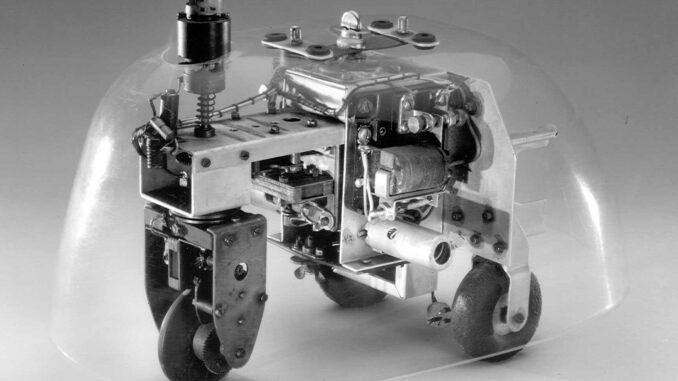
\includegraphics[width=0.4\textwidth]{images/tortugas_william_grey.jpg}
    \caption{Interior de los robots "tortuga". Fuente: alpoma.net}
    \label{fig:tortugas_grey}
\end{figure}


Otro hito importante en este campo fue el desarrollo de la furgoneta autónoma Mercedes-Benz de Ernst Dickmanns y su equipo en la década de 
1980~\Cite{ernst80}. Este vehículo, \textbf{figura \ref{fig:furgoneta_ernst}}, equipado con sensores y sistemas de control avanzados, fue capaz de navegar de forma autónoma por 
carreteras y seguir a otros vehículos con un alto grado de precisión, sentando las bases para los sistemas de conducción autónoma modernos. 
Este vehículo fue   incluso capaz de circular por una ''autobahn'' alemana a 90 km/h

\begin{figure}[h]
    \centering
    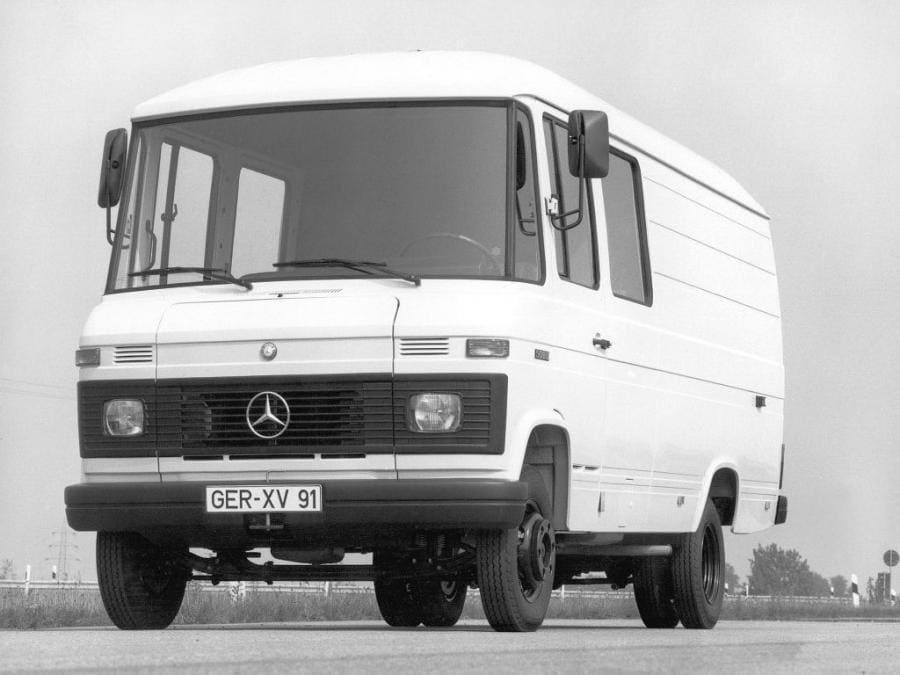
\includegraphics[width=0.5\textwidth]{images/furgoneta_ernst_dickens.jpeg}
    \caption{Furgoneta Autónoma creada por Ernst Dickmanns. Fuente: ~\cite{ernst80}.}
    \label{fig:furgoneta_ernst}
\end{figure}

En el ámbito militar, la Agencia de Proyectos de Investigación Avanzada de Defensa (DARPA) de los Estados Unidos ha desempeñado un 
papel crucial en el impulso de la robótica y la navegación autónoma. Uno de los proyectos emblemáticos de DARPA fue el primer vehículo 
que funcionaba mediante un radar, un láser, y visión computarizada. En 1987, los laboratorios HRL demostraron que se podía construir un 
vehículo que podía diseñar su propia ruta una vez que se salía del mapa~\cite{DARPA20}. El vehículo pudo moverse más de 600 metros a través de terreno 
complejo como pendientes, grandes rocas y vegetación.


Pronto grandes empresas como Google, Audi o más adelante Tesla iniciaron una nueva revolución en el mundo de la conducción autónoma, 
introduciendo los conceptos de \textit{machine learning} o \textit{deep learning} en sus vehículos como una nueva forma de toma de 
decisiones, de esta manera los vehículos primero aprendían por si mismos a que decisiones tomar en cada situación en base a un entrenamiento, 
esto dio lugar a una gran ventaja ya que, en este campo la programación clásica era inviable por la gran cantidad de posibilidades que existen.

Audi comenzó esta travesía con su modelo RS7 autónomo~\cite{audirs715}, que recorrió a una velocidad de 240 km/h el circuito de Hockenheim en Alemania. 
Siendo este 5 segundos más rápido que un un vehículo tripulado por un conductor profesional. Le siguió Google con una flota de 25 
vehículos autónomos que sin superar los 40 km/h recorrieron las calles de Mountain View, California.

Más adelante salieron empresas como Waymo~\cite{waymo24}, que empezaron a desarrollar el concepto de taxi autónomo o Tesla con sus vehículos que 
incorporan el conocido \textbf{Autopilot}. Este utiliza una combinación de cámaras, radares y sensores para ofrecer características 
avanzadas de asistencia al conductor, como el piloto automático adaptativo y la asistencia de cambio de carril.

\section{Nav2: Stack para navegación autónoma de robots móviles}
ROS es un SDK o framework para el desarrollo de software en robots, fue desarrollado en 2007 en la universidad de Standford para 
dar soporte a un proyecto interno, desde el 2008 ha sido mantenido principalmente por Willow Garage, una incubadora de empresas y 
laboratorio de investigación robótica, aunque por su naturaleza de código abierto el crecimiento y el mantenimiento ha sido una labor 
común de sus usuarios~\cite{ros2}.

ROS2 funciona en base a Nodos, programados en C++ o Python, estos comprenden los llamados paquetes y el conjunto de paquetes es un stack, 
uno de los stacks más conocidos, usados y mejorados es el utilizado en este trabajo, Nav2 o Navigation2~\cite{nav2}~, que en ya su segunda 
versión es la opción más utilizada para la creación de algoritmos de navegación autónoma.
Este stack tiene todo lo necesario para crear un sistema robusto de navegación autónoma, principalmente en interiores pero también para exteriores con pequeñas modificaciones.

El stack posee soporte para todo tipo de robots (Ackermann, Diferencial, Humanoide, Omni-direccional), aquí nos referiremos a los planificadores locales
como ''controladores'' y a los planificadores globales como simplemente ''planificadores''. Nav2 cuenta con controladores muy rápidos y 
sencillos como el DWB (Dynamic Window Approach) que funciona exclusivamente para robots con posibilidad de giro \textit{in situ}, TEB 
(Time Elastic Band) o el famoso RPP (Regulated Pure Pursuit) que aunque sencillos ya nos permiten una configuración más avanzada
para el caso que aquí se presenta, como es el radio de giro mínimo, hasta otros mucho más complejos como el MPPI (Model Predictive Path Integral), un algoritmo 
muy robusto que usa un método de predicción en el tiempo para navegación de vehículos a grandes velocidades. Por otro lado tenemos los 
planificadores donde existen varias versiones de 2 algoritmos también muy conocidos, el A* y el Theta*~\cite{sun2023path}.

En su primera versión usaba una máquina de estados finita como lógica de actuación, una solución muy bien estudiada por su antigüedad
pero que su modificación para un problema concreto resultaba complicada. Por ello, en su nueva versión se utilizan los llamados 
\textit{behavior trees}~\cite{colledanchise2018behavior}, unas estructuras lógicas muy versátiles y sobre todo extremadamente adaptables, 
gracias a ello el stack de navegación permite una configuración absoluta de todos sus componentes, desde la creación de planificadores locales, globales o
plugins para añadir comportamientos hasta, capas para los mapas de coste, suavizadores de trayectoria o incluso la creación o modificación de los 
propios árboles de comportamiento. Su estructura funciona por bloques como se muestra en la  \textbf{figura \ref{fig:nav2_arch}}.
\begin{figure}[h]
    \centering
    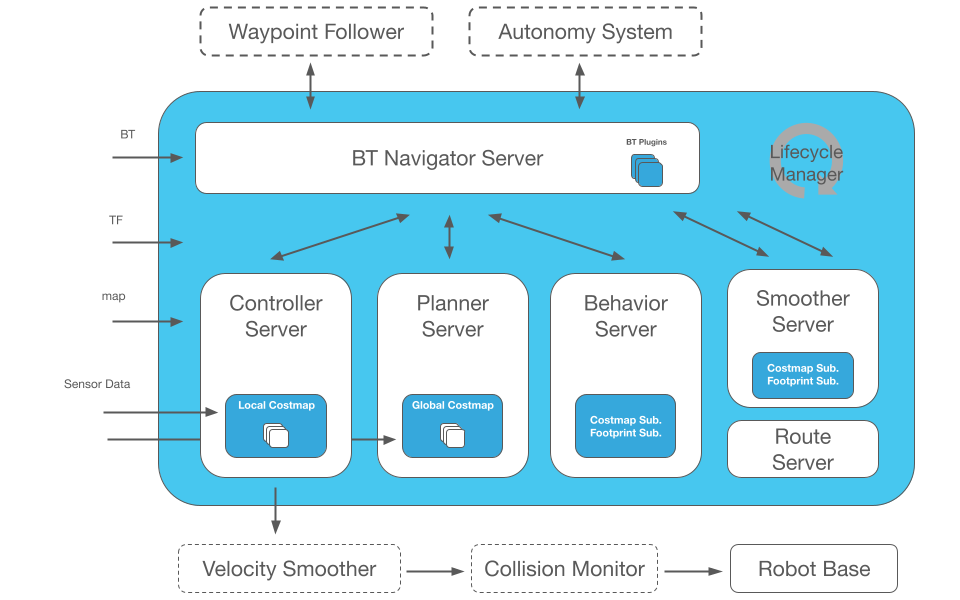
\includegraphics[width=0.8\textwidth]{images/nav2_architecture.png}
    \caption{Arquitectura interna de Nav2. Fuente:~\cite{nav2}}
    \label{fig:nav2_arch}
\end{figure}
\newpage
\section{Localización}
La localización se conoce como uno de los principales y más complejos problemas de la robótica móvil. Se basa en un concepto 
muy sencillo, saber donde se encuentra el robot, una tarea que depende del entorno, de las condiciones y de los sensores disponibles, 
pudiendo así suponer una gran problemática. Por ello, durante los años se han desarrollado multiples técnicas de localización para intentar mitigar este 
gran problema, aquí se exponen los principales métodos usados a día de hoy en robótica.

\subsection{SLAM: Simultaneous Localization And Mapping}
El método SLAM, es un método utilizado en robótica y campos relacionados para que un agente móvil (como un robot) pueda construir un mapa de un 
entorno desconocido y al mismo tiempo determinar su propia posición respecto de ese mapa.

El proceso comienza con una estimación inicial de la posición del robot y el mapa del entorno. Esta estimación puede ser rudimentaria y 
se mejora a medida que el robot explora y recopila más datos, más adelante sucede una captura de datos donde el agente móvil o robot, utiliza sus 
sensores como cámaras, Lidar o diferentes fuentes de odometría para capturar información sobre la disposición del entorno y de su propia 
posición. A partir de los datos capturados se construye un modelo del entorno que puede estar en 2 o 3 dimensiones. A medida que el agente móvil se mueve 
y recopila más datos, el mapa y la estimación de la posición se actualizan continuamente para reflejar el conocimiento más reciente del 
entorno y la ubicación del agente. El algoritmo incluye técnicas avanzadas de fusión sensorial, estimación probabilística y optimización 
para lograr una localización y un mapeo precisos.

Este método es uno de los más usados en navegación en interiores donde hay muchos objetos y referencias para que este algoritmo pueda 
''localizarse''. El principal problema recae al intentar usarlo en exteriores, donde suele haber pocas referencias o están mucho más 
espaciadas, donde el ruido es mucho mayor y existen más fuentes, pero sobre todo, donde la idea de mapear un entorno tan extenso se vuelve 
inviable para la mayoría de situaciones.

\subsection{AMCL: Adaptive Monte Carlo Localization}

AMCL es un método probabilístico para la localización de robots que utiliza un enfoque de Monte Carlo (también conocido como filtro de 
partículas). A diferencia de otros métodos, AMCL puede adaptarse dinámicamente a la incertidumbre y las fluctuaciones en el entorno. 

Primeramente se genera un conjunto de partículas que representas las posiciones probables del robot en función a una distribución uniforme, 
cada partícula se actualiza de acuerdo con el movimiento esperado del robot. Esto se logra aplicando las entradas de control del robot y 
considerando la incertidumbre del movimiento. Las partículas se ponderan de acuerdo con su probabilidad de ser correctas. Las partículas 
con mayor probabilidad se duplican, mientras que las partículas con menor probabilidad se eliminan. 

AMCL es un método flexible y robusto, puede proporcionar una estimación precisa de la posición del robot incluso en condiciones cambiantes. 
Una gran desventaja es que necesita al igual que SLAM un mapa del entorno, algo poco viable en exteriores como ya se ha comentado.

\subsection{Fusión de odometrías mediante filtros extendidos de Kalman}

En la fusión de odometrías con filtros extendidos de Kalman, se utiliza un modelo del sistema y mediciones provenientes de múltiples fuentes para estimar su estado,
 que en este caso, sería la posición y la orientación del robot.

El filtro de Kalman es un algoritmo predictivo y recursivo desarrollado por Rudolf E. Kalman en 1960. Este algoritmo sirve para identificar el ''estado oculto'' o no medido de un sistema dinámico \textbf{lineal} teniendo en cuenta las varianzas de 
los ruidos que afectan al sistema (errores en las mediciones del sistema de sensado), este algoritmo conlleva 2 partes 
bien definidas, la primera es una predicción de estados donde dada una matriz que relaciona el estado anterior con el estado presente 
se calcula una estimación de estados y una matriz de varianzas \textit{a priori} y posteriormente una etapa de corrección mediante una 
medición para calcular el llamado residuo de medición y la \textit{ganancia de Kalman}, 
que a diferencia de otros métodos~\cite{wikiLuenberg} tiene la ventaja de ser calculada dinámicamente en base a la información del error (matriz de covarianzas). 
Finalmente se corrige la estimación y se repite el proceso.

En el caso de sistemas dinámicos \textbf{no lineales} es posible usar una modificación del filtro conocida por ''filtro extendido de Kalman o EKF''~\cite{rigatos2007extended}, donde 
se linealiza entorno al estado actual y donde antes teníamos una matriz que relaciona el estado anterior con el actual ahora tenemos la función \textit{f} 
para la predicción de estados y su \textit{Jacobiana} (\textbf{F}) para la predicción de varianzas~(\ref{eq:prediccion_estado} y \ref{eq:prediccion_covarianza}).

Para la segunda etapa también tendremos otra función \textit{h} y su \textit{Jacobiana} (\textbf{H}) que representan la relación entre 
las mediciones y el estado actual que, sumado a la matriz de varianzas \textbf{R} nos otorga la actualización de estados y de covarianza (\ref{eq:ganancia_kalman}, \ref{eq:actualizacion_estado} y \ref{eq:actualizacion_covarianza}). 

% Predicción del estado
\begin{equation}\label{eq:prediccion_estado}
\hat{x}_k^- = f(\hat{x}_{k-1}, u_k) 
\end{equation}
\begin{equation}\label{eq:prediccion_covarianza}
P_k^- = F_{k-1}P_{k-1}F_{k-1}^T + Q_{k-1}
\end{equation}

% Actualización de la medición
\begin{equation}\label{eq:ganancia_kalman}
K_k = P_k^-H_k^T(H_kP_k^-H_k^T + R_k)^{-1}
\end{equation}
\begin{equation}\label{eq:actualizacion_estado}
\hat{x}_k = \hat{x}_k^- + K_k(z_k - h(\hat{x}_k^-))
\end{equation}
\begin{equation}\label{eq:actualizacion_covarianza}
P_k = (I - K_kH_k)P_k^-
\end{equation}
Donde :

\begin{itemize}
    \item \( \hat{x}_k^- \): Predicción del estado a priori en el instante de tiempo \( k \).
    \item \( \hat{x}_{k-1} \): Estado estimado en el instante de tiempo anterior \( k-1 \).
    \item \( P_k^- \): Predicción a priori de la covarianza del estado en el instante de tiempo \( k \).
    \item \( P_{k-1} \): Covarianza del estado en el instante de tiempo anterior \( k-1 \).
    \item \( Q_{k-1} \): Covarianza del ruido del proceso en el instante de tiempo \( k-1 \).
    \item \( K_k \): Ganancia de Kalman en el instante de tiempo \( k \).
    \item \( R_k \): Covarianza del ruido de medición en el instante de tiempo \( k \).
    \item \( \hat{x}_k \): Estado estimado en el instante de tiempo \( k \) después de la corrección.
    \item \( F_{k-1} = \frac{\partial f}{\partial x}\Bigg|_{x=\hat{x}_{k-1}} \): Matriz Jacobiana de la función de transición de estado.
    \item \( H_k = \frac{\partial h}{\partial x}\Bigg|_{x=\hat{x}_k^-} \): Matriz Jacobiana de la función de observación.
\end{itemize}



\section{Sistemas sensoriales para Navegación Autónoma}

Un robot requiere siempre de un sistema que le permita interactuar con el entorno, detectarlo y analizarlo. Es por ello que la sensorización 
también es una parte fundamental en robótica. El esquema de sistemas sensoriales para uso en robótica móvil y más concretamente en navegación 
puede variar pero fundamentalmente requiere, por un lado, de una fuente de localización sin error acumulativo y otra fuente de odometría que proporcione posición y orientación 
de manera rápida y por otro lado, algún tipo de sistema que sea capaz de analizar el entorno. Para ello, se ha dispuesto un sistema sensorial 
compuesto por 3 fuentes sensoriales que recopilan estas necesidades.
\subsection{Lidar}
En los inicios de la robótica los principales sensores para la medición de distancias eran los sónares pero conforme la tecnología ha ido avanzando 
cada vez más se han reemplazando por los sensores Lidar gracias a su precisión y utilidad en gran cantidad de situaciones. 
Estos sensores son capaces de hacer un barrido horizontal de hasta 360º y algunos un barrido vertical como el utilizado en este proyecto. 
Han sido utilizados tanto para detección de obstáculos, localización en el mundo o incluso para el mapeado de entornos, son muy interesantes 
por su buena relación entre rango y precisión, siendo algunos capaces de funcionar en exteriores de manera muy precisa.

\begin{figure}[H]
    \centering
    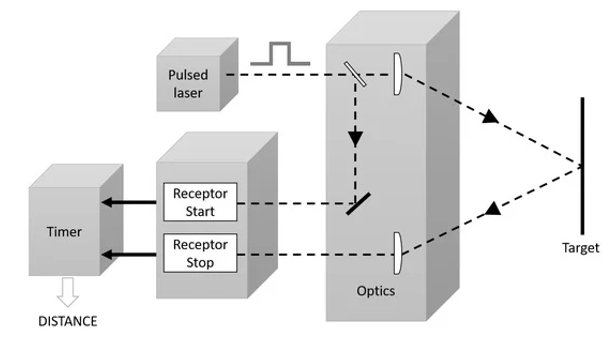
\includegraphics[width=0.5\textwidth]{images/lidar_explicacion.png}
    \caption{Esquema teórico de funcionamiento de un Lidar 1D, Fuente: Pyrois Tech}
    \label{fig:lidar_explicacion}
\end{figure}

Estos sensores son agrupados con el nombre de ''sensores de tiempo de vuelo'' y es que su funcionamiento se basa en eso precisamente. Están 
dotados de un laser pulsado y un receptor junto con un sistema óptico de lentes y espejos~\ref{fig:lidar_explicacion}, el láser emite un rayo de luz concentrada que viaja 
hasta el objeto a detectar, rebota en el y vuelve hasta ser detectado por el receptor del dispositivo, de esta manera conociendo que la 
velocidad de la luz es \begin{math}c=299.792.458 m/s\end{math} podemos definir la distancia al objeto (\textbf{D}) como:~$$D = c * \Delta{t} / 2$$ Si a esto 
le añadimos un motor eléctrico que haga rotar todo el dispositivo a gran velocidad alrededor de un eje obtenemos un 
barrido del entorno~\ref{fig:lidar3d}.


\begin{figure}[h]
    \centering
    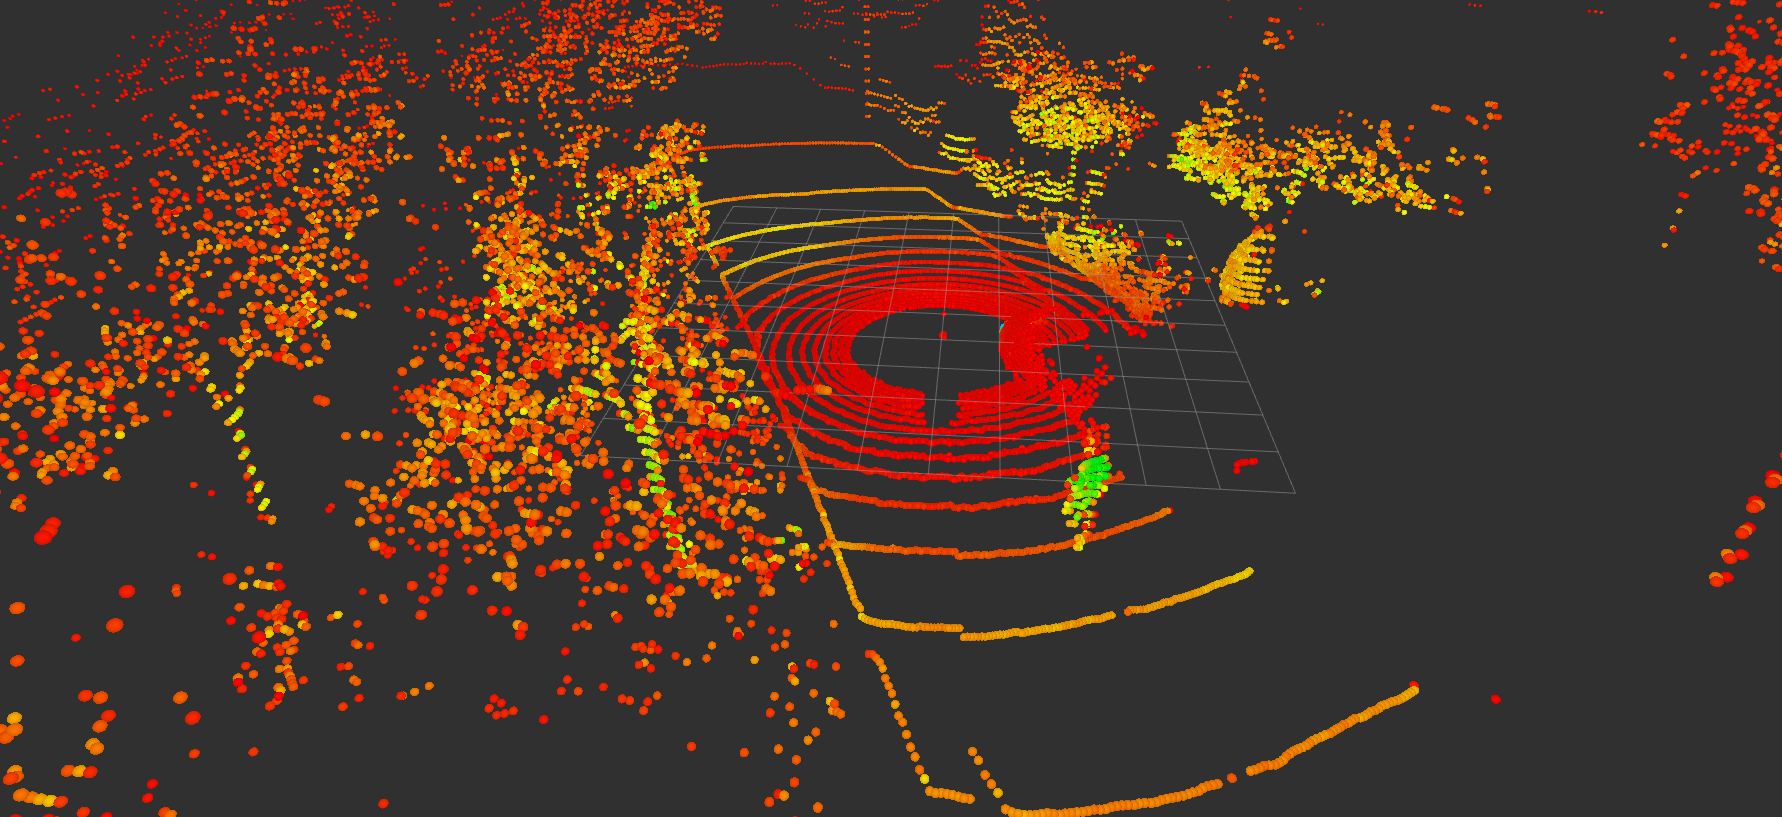
\includegraphics[width=0.5\textwidth]{images/lidar3d_1.png}
    \caption{Nube de puntos de un Lidar 3D. Fuente: propia}
    \label{fig:lidar3d}
\end{figure}

\subsection{GPS}

El GPS es una herramienta bien conocida, estudiada y utilizada por una gran variedad de sectores, y aunque es una tecnología que funciona 
muy bien tiene sus limitaciones y problemas. Necesita una vista clara del cielo, lo cual no siempre es posible, las frecuencias a las que trabajan 
suelen ser muy bajas, del orden de unos pocos hercios, lo que dificulta conseguir una posición continua necesaria en 
la mayoría de casos para una correcta navegación. 

Por otro lado, la precisión tampoco suele ser muy buena excepto que se utilizen tecnologías más avanzadas como son los 
GPS RTK (Real Time Kinematic, ~\textbf{figura \ref{fig:rtk_tech}}), que mejora su error al añadir un protocolo de correcciones por medio de radio, modem o wifi en base a una 
estación fija de la que se conoce con gran exactitud sus coordenadas GPS, otorgando así hasta una precisión de unos pocos centímetros. Aún así, 
normalmente es muy necesario usarlo en conjunto con otros sensores, sean varios GPS, IMUs o con técnicas más avanzadas de localización 
como el conocido SLAM (SImultaneous Localization and Mapping), AMCL (Adaptative Montecarlo localization) o el utilizado en el presente 
proyecto, la fusión de fuentes de odometría basada en filtros extendidos de Kalman (EKF).

\begin{figure}[h]
    \centering
    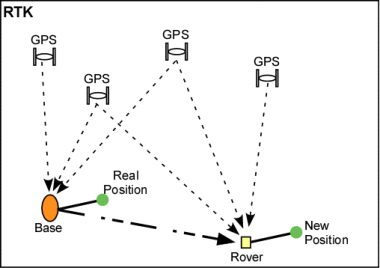
\includegraphics[width=0.5\textwidth]{images/rtk_arquitecture.png}
    \caption{Esquema de tecnología RTK. Fuente: ResearchGate}
    \label{fig:rtk_tech}
\end{figure}

\subsection{IMU}

Las \textit{Inertial Motion Units} son un conjunto de sensores que normalmente existen en 2 configuraciones, 6 grados de libertad, 
donde encontramos un giroscopio y un acelerómetro o 9 grados de libertad, donde además se encuentra un magnetómetro.

En base a estos 2 o 3 sensores se puede calcular una orientación ya sea relativa desde el inicio del movimiento o absoluta respecto del norte 
magnético, estas unidades aunque son muy necesarias tienen una gran desventaja y es que son afectadas por un error acumulativo 
(error Abbe)~\cite{errorAbbe23}, agregando cambios a la medición, lo que se conoce como deriva, esta deriva es muy perjudicial para conseguir una 
correcta localización por lo que al igual que comentamos anteriormente la fusión con otros sensores o técnicas de localización resulta muy necesaria.
\cleardoublepage
\titlespacing*{\chapter}{0pt}{-50pt}{40pt} % Ajusta los márgenes y espaciados
% \titlespacing*{\section}{0pt}{-50pt}{40pt} % Ajusta los márgenes y espaciados

\chapter{Desarrollo}

\section{Diseño del sistema sensorial}

EL robot considerado en este trabajo fin de grado esta montado sobre una plataforma móvil adquirida a la empresa \textbf{Agilex}, \textbf{figura \ref{fig:hunter}}, en concreto el 
modelo Hunter V2.0, un robot móvil tipo \textbf{Ackermann} muy resistente diseñado para cargas pesadas y escenarios de conducción precisos 
a baja velocidad, sus dimensiones son 980 x 745x 380mm, tiene una carga máxima de 150 kg y una velocidad máxima de 1.5 m/s, un radio 
de giro mínimo de 1.6 m y una autonomía de 22 km. El robot incluye un software para el cálculo de la cinemática inversa, la publicación de 
la odometría de los \textit{encoders} de las ruedas por el topic \textit{/hunter/odom} y la suscripción de un mensaje tipo \textit{sensor\_msgs/Twist} 
para comandar velocidades angulares y lineales por el topic \textit{cmd\_vel}. La comunicación al ordenador de abordo se realiza mediante \textbf{Bus CAN}. 
En la \textbf{figura \ref{fig:datasheet_hunter}} se pueden observar las especificaciones del vehículo completas. Si bien se ha usado este robot y su sistema sensorial 
se podría adaptar a cualquier otro de similares características.


\begin{figure}[H]
    \centering
    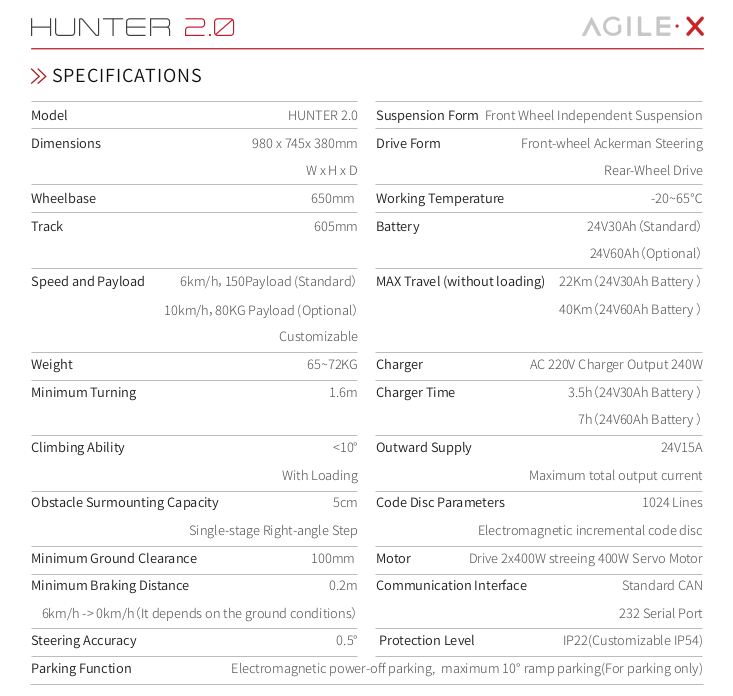
\includegraphics[width=0.8\textwidth]{images/hunter_datasheet.png}
    \caption{Hoja de datos de la base del vehículo. Fuente: AgileX}
    \label{fig:datasheet_hunter}
\end{figure}

\begin{figure}[h]
    \centering
    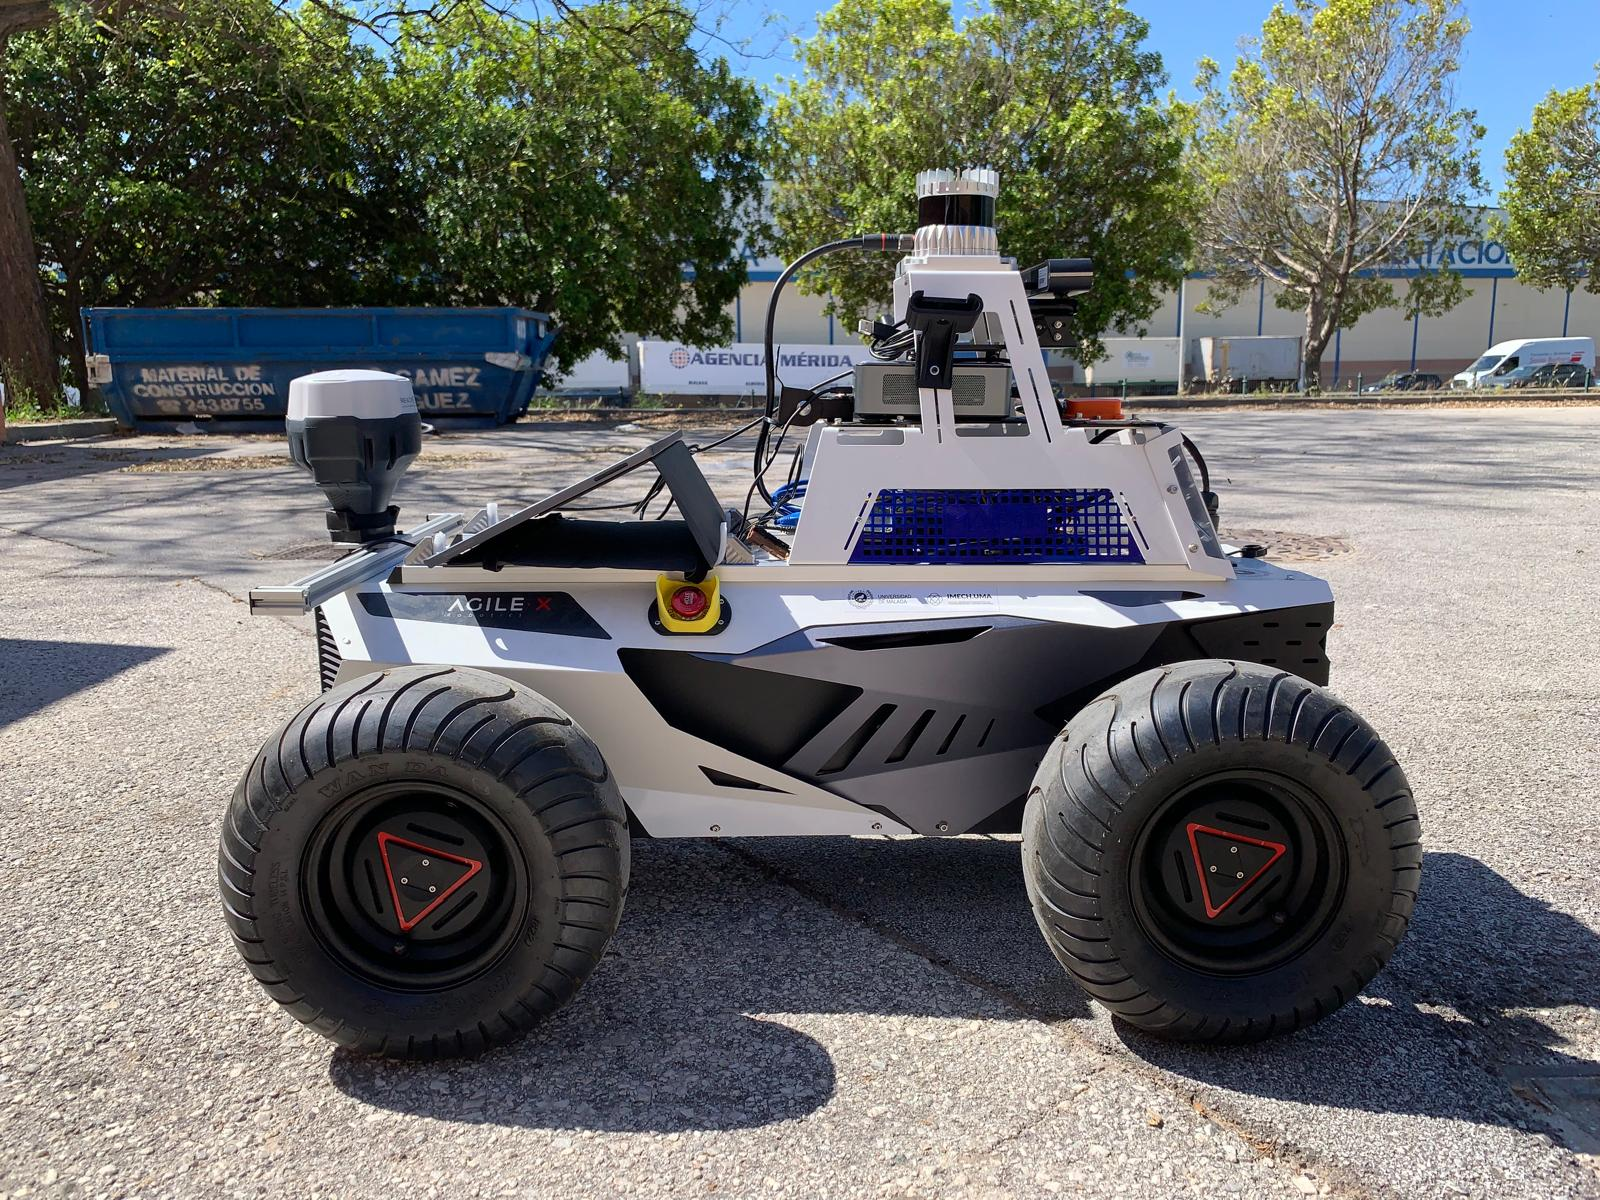
\includegraphics[width=0.5\textwidth]{images/hunter_v2.jpeg}
    \caption{Chasis del vehículo autónomo. Fuente: propia}
    \label{fig:hunter}
\end{figure}

El ordenador de abordo actualmente es un mini ordenador de la marca minis forum, un ordenador super ligero y versátil con altas 
prestaciones, incorpora Linux como sistema operativo, requisito fundamental para utilizar ROS2. El ordenador cuenta con una 
memoria RAM de 16MB y una memoria ROM SSD de 512GB, un procesador Ryzen 5 3550H de la marca AMD con una velocidad de 2.1GHz, 6 puertos USB-A, 
1 puerto USB-C, conectores HDMI Y DP, 2 entradas para Ethernet y módulos WiFI y Bluetooth.

\subsection{Lidar 3D Ouster}
En primer lugar contamos con un LIDAR 3D de la marca Ouster, \textbf{figura \ref{fig:ouster_hunter}}, en concreto el 
modelo de medio alcance, con un rango que se comprende entre los 0.4 y los 120 metros, está preparado para exteriores con una visera 
protectora y es capaz de barrer áreas en 360º horizontalmente y 45º verticalmente, funciona a 
100Hz y tiene una resolución de 2 cm de media ya que depende de la distancia, todos estos datos se pueden comprobar también en la~\textbf{figura \ref{fig:datasheet_ouster}}, 
para la implementación con ROS2 se usó el driver oficial de la empresa. 

\begin{figure}[h]
    \centering
    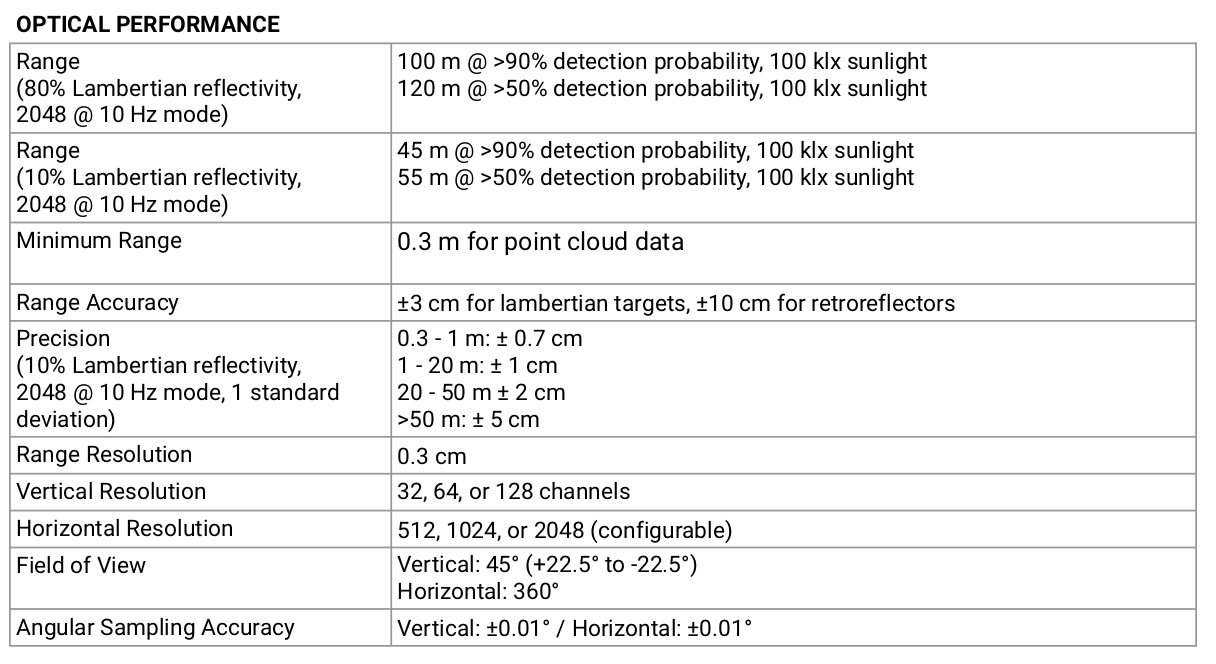
\includegraphics[width=0.5\textwidth]{images/osuter_datasheet.png}
    \caption{Hoja de datos del Ouster OS1-32-U. Fuente: Ouster}
    \label{fig:datasheet_ouster}
\end{figure}

\begin{figure}[H]
    \centering
    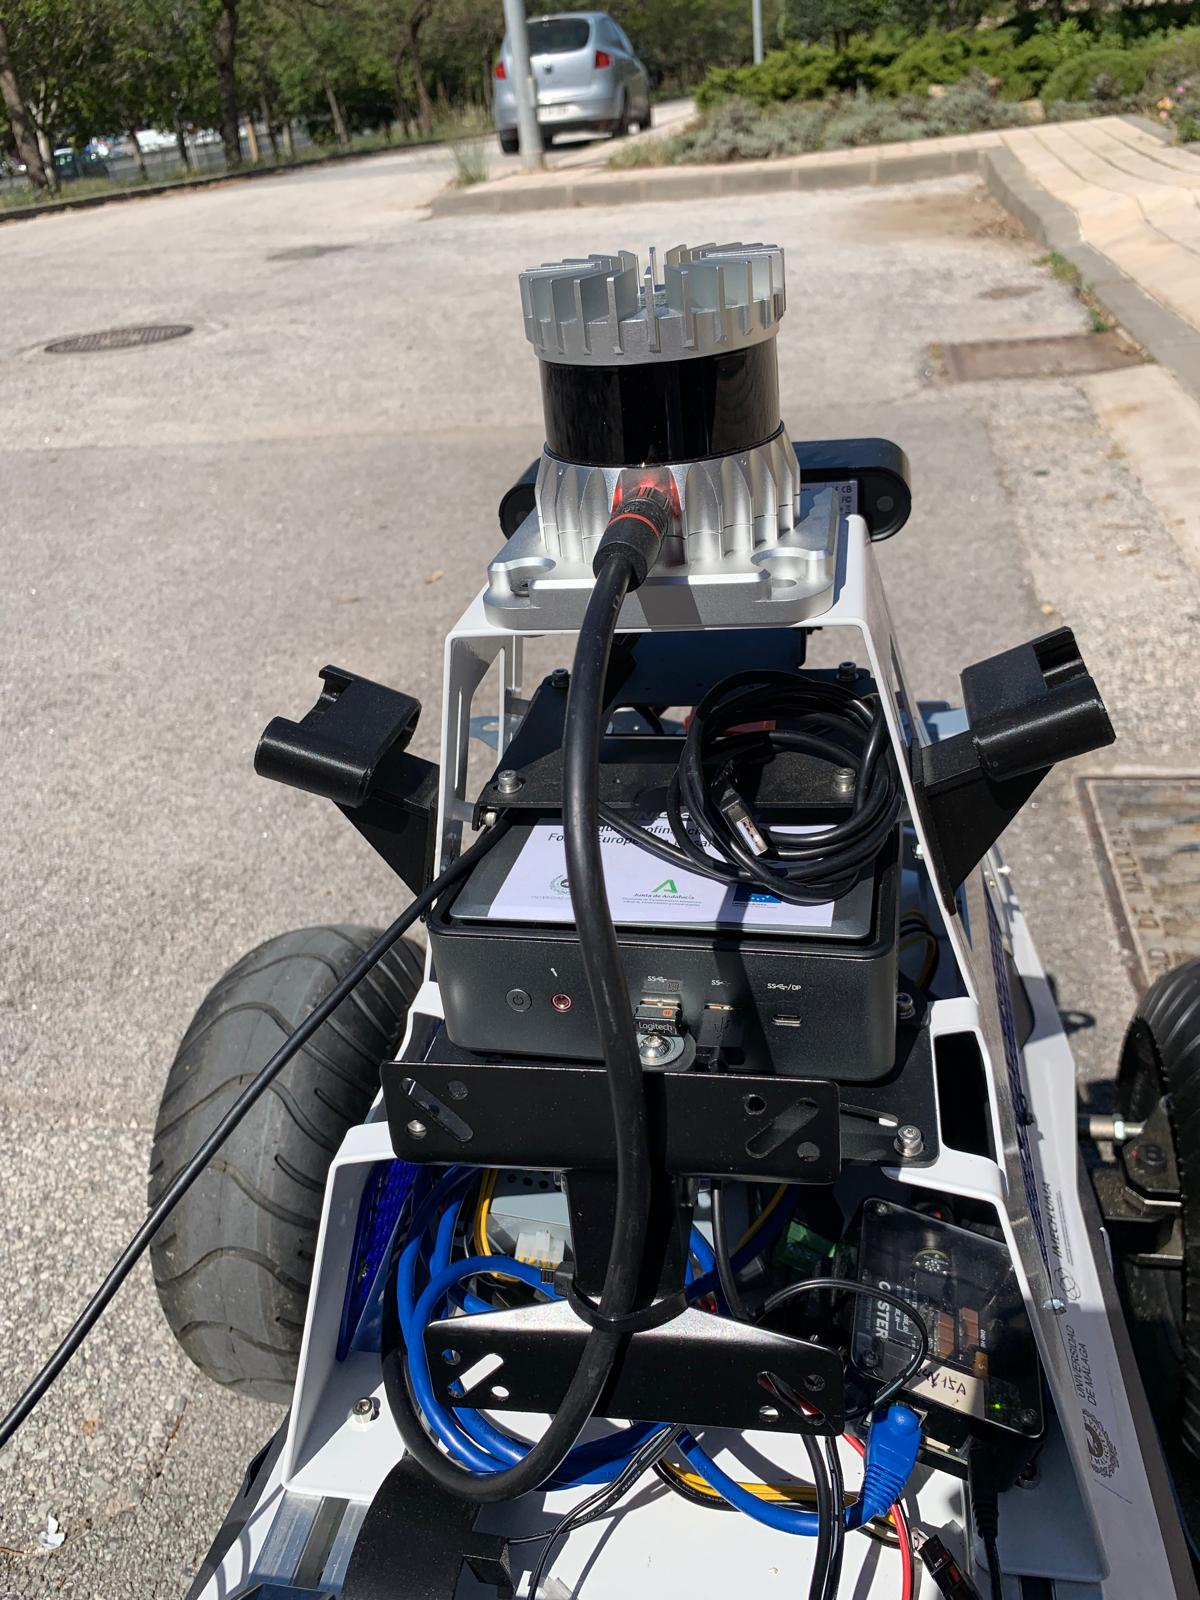
\includegraphics[width=0.4\textwidth]{images/ouster_hunter.jpeg}
    \caption{Ouster montado en la torre del vehículo. Fuente: propia}
    \label{fig:ouster_hunter}
\end{figure}

A parte del sensor láser este también tiene incorporado una IMU de 6 grados de libertad, 3 para un giroscopio y 3 para un acelerómetro, 
decir que esta unidad de medición inercial fue la única usada durante el 90\% del proyecto lo cual, dificultó mucho la obtención de una 
buena localización a causa no incluir un magnetometro y de no ser de muy alta gama, de todas formas como se explica más adelante se 
consiguió una buena orientación usando este dispositivo. Fue colocado en la torre del robot para máxima visibilidad del Lidar.

En las \textbf{figuras \ref{fig:lidar_2d_pruebas} y \ref{fig:lidar_3d_pruebas}} se observan las pruebas que se hicieron con el vehículo en el recinto 
de la universidad donde para el mismo sitio se puede ver la diferencia entre las salidas de barrido láser y nube de puntos en 3 dimensiones.



\begin{figure}[htbp]
  \centering
  \begin{minipage}[b]{0.45\textwidth}
    \centering
    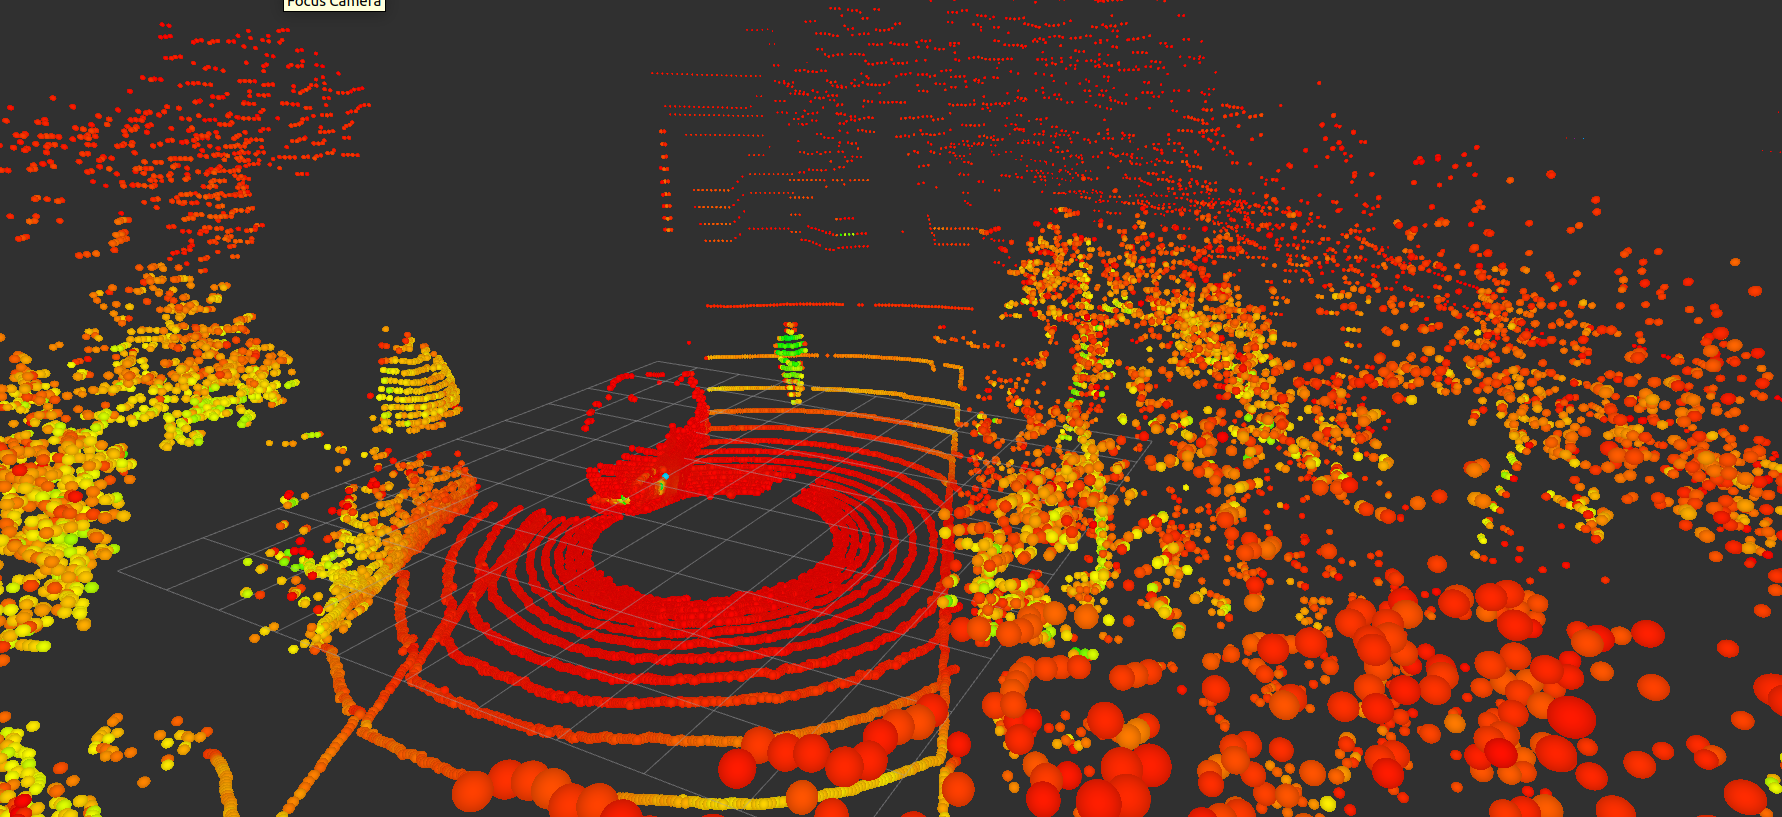
\includegraphics[width=\textwidth]{images/lidar3d_2.png}
    \caption{Salida de Lidar 3D en el recinto de la facultad de Telecomunicaciones. Fuente: propia}
    \label{fig:lidar_2d_pruebas}
  \end{minipage}
  \hfill
  \begin{minipage}[b]{0.45\textwidth}
    \centering
    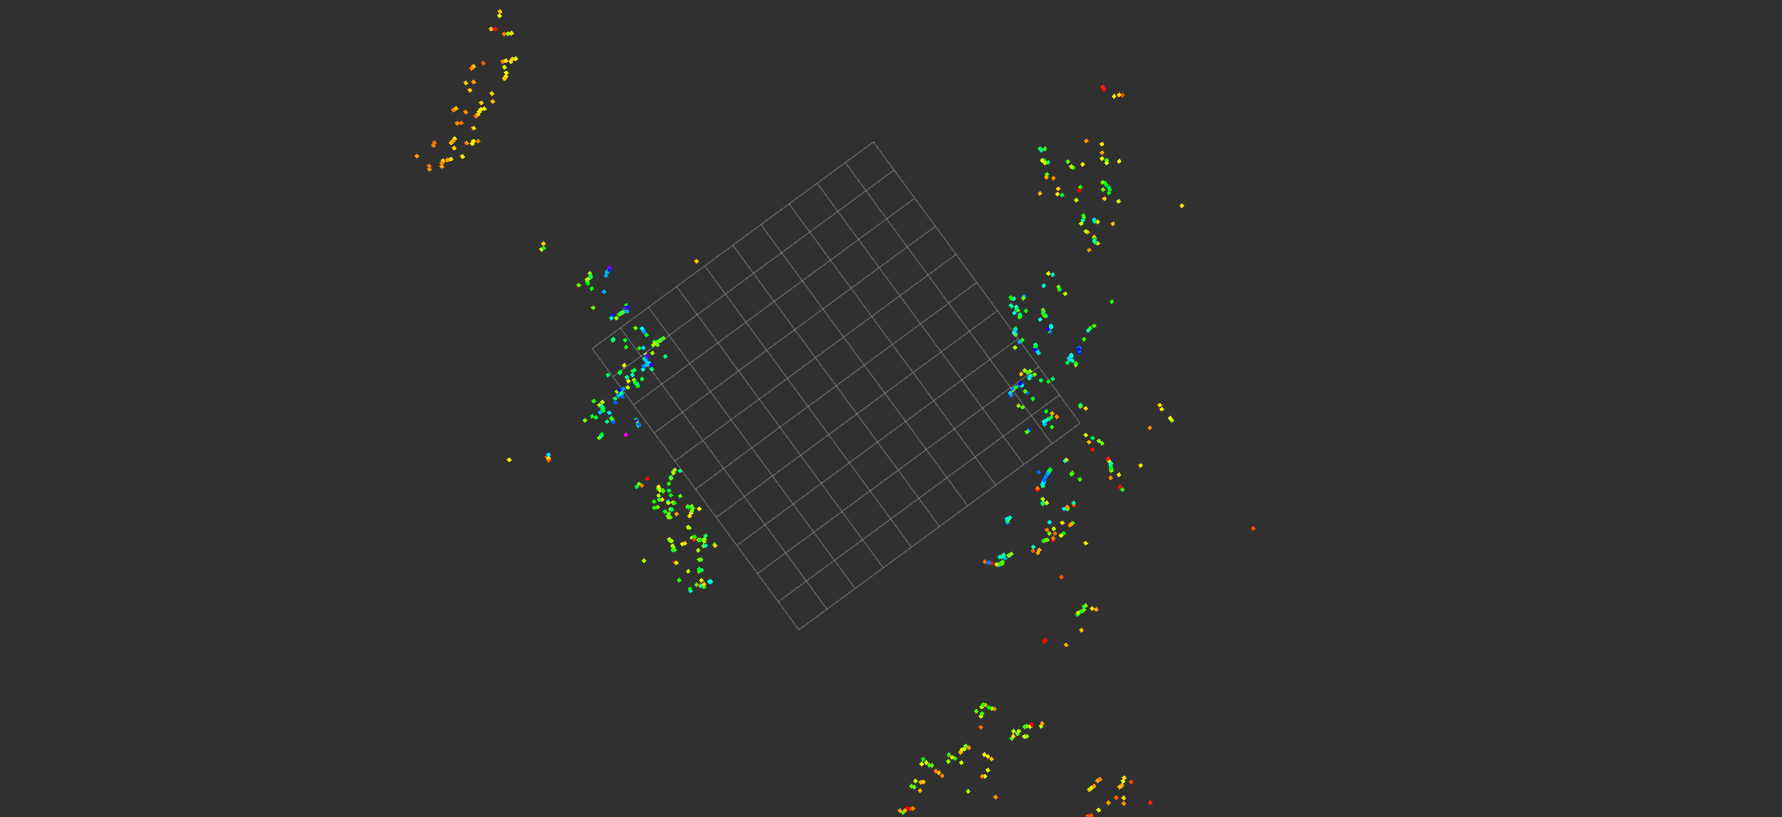
\includegraphics[width=\textwidth]{images/lidar2d.png}
    \caption{Salida de Lidar 2D en el recinto de la facultad de Telecomunicaciones. Fuente: propia}
    \label{fig:lidar_3d_pruebas}
  \end{minipage}
\end{figure}

En cuanto al esquema de comunicación con el software, el driver usado publica los siguientes mensajes de datos.
\begin{itemize}
    \item Lidar 2D, un mensaje de tipo \textit{sensor\_msgs/LaserScan} por el topic \textit{/ouster/scan}
    \item Lidar 3D, un mensaje de tipo \textit{sensor\_msgs/PointCloud} por el topic \textit{/ouster/points}
    \item IMU, un mensaje de tipo \textit{sensor\_msgs/Imu} por el topic \textit{/ouster/imu}
\end{itemize}

\subsection{GPS RTK Reach RS2+}

El GPS utilizado fue un GPS Reach RS2+, \textbf{figura \ref{fig:reach_rs2}}, con tecnología RTK basado en el protocolo NTRIP para la 
corrección de posicionamiento. Este GPS funciona usando el protocolo NMEA, un protocolo extremadamente robusto utilizado en el sector marino, 
cuenta con una frecuencia máxima de 5Hz y una precisión de hasta 1 cm, \textbf{figura \ref{fig:datasheet_reach}}. Para su montaje se creó un soporte con un perfil de aluminio al que 
se le atornilló el propio sensor, de manera que tenga una visión clara del cielo en todo momento y que a la vez no interfiera con la linea de 
corte del Lidar, su implementación en ROS2 también viene ampliamente documentada ya que el protocolo usado (NMEA) es muy conocido, 
para su conexionado se pueden usar varios métodos, como Wifi o radio pero para este proyecto se implementó el serial por medio de USB para 
minimizar las interferencias y pérdidas de señal. Para la comunicación se tiene un solo mensaje de interés, este es de tipo \textit{sensor\_msgs/NavSatFix} 
y se publica por el topic \textit{/hunter/fix}.


\begin{figure}[htbp]
  \centering
  \begin{minipage}[b]{0.35\textwidth}
    \centering
    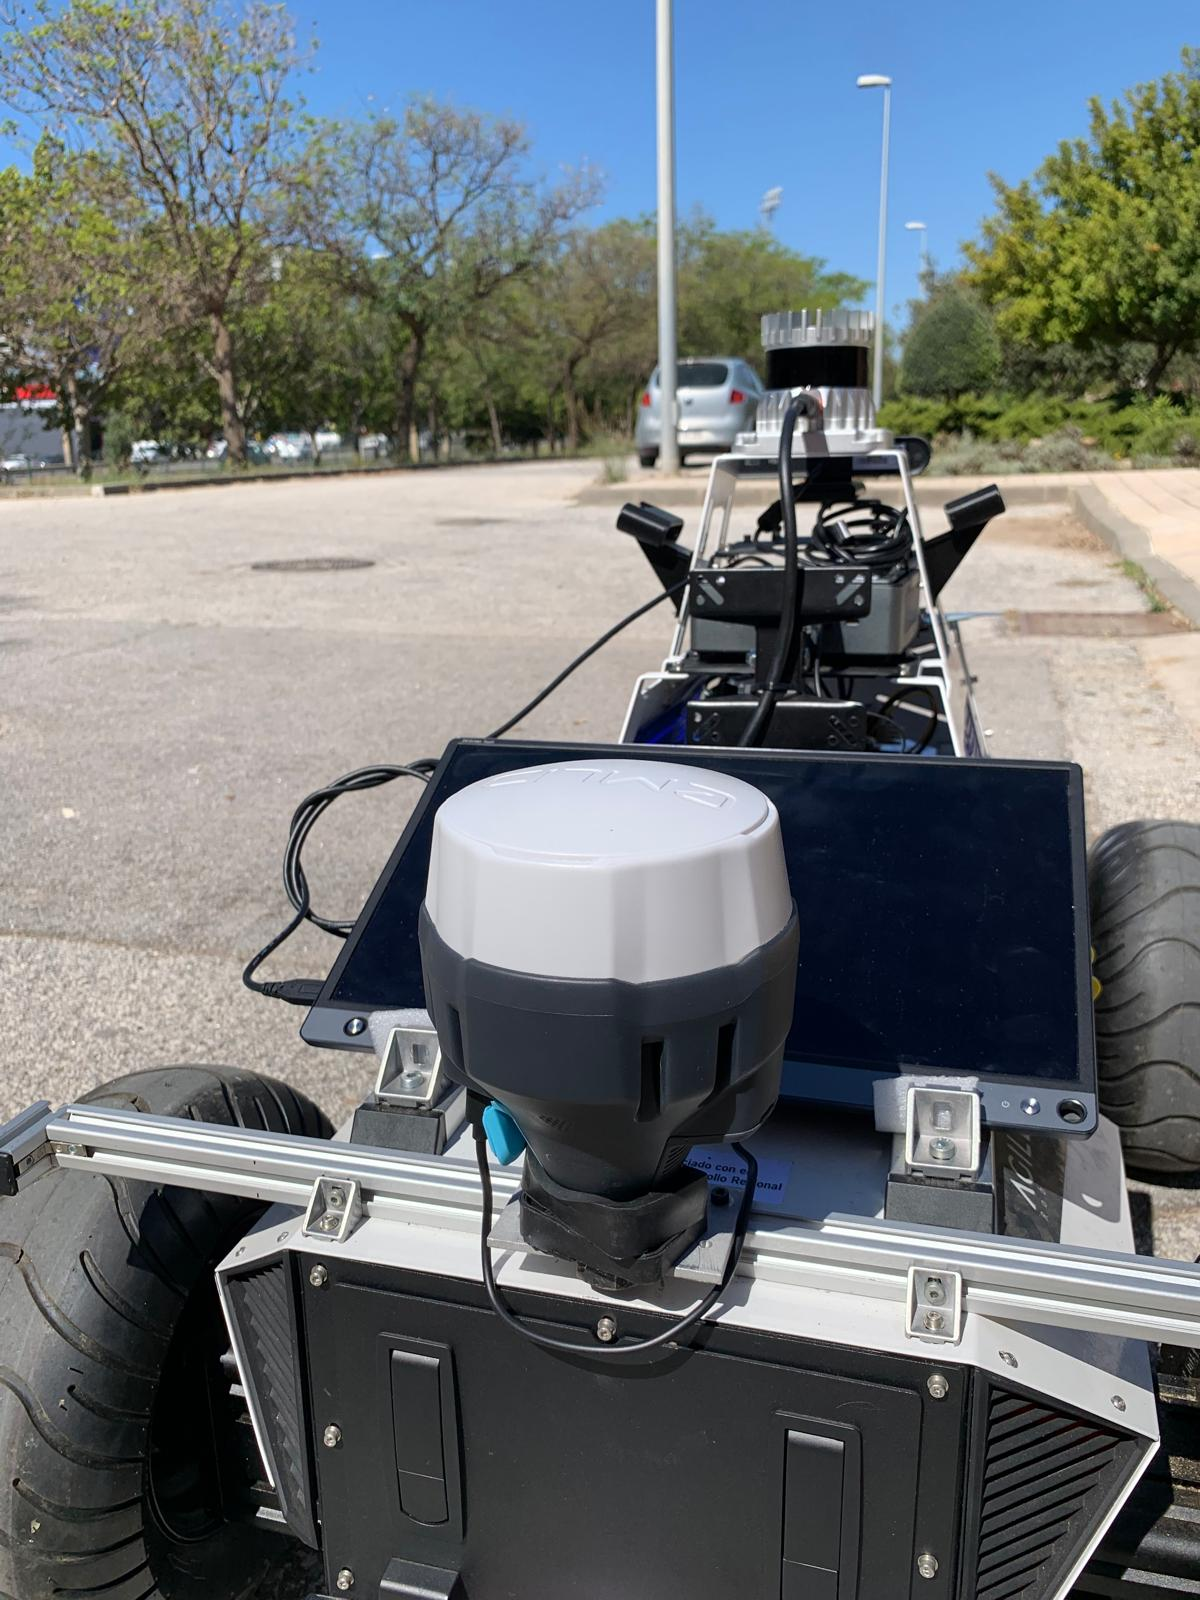
\includegraphics[width=\textwidth]{images/reach_rs2.jpeg}
    \caption{GPS Reach RS2+. Fuente: propia}
    \label{fig:reach_rs2}
  \end{minipage}
  \hfill
  \begin{minipage}[b]{0.5\textwidth}
    \centering
    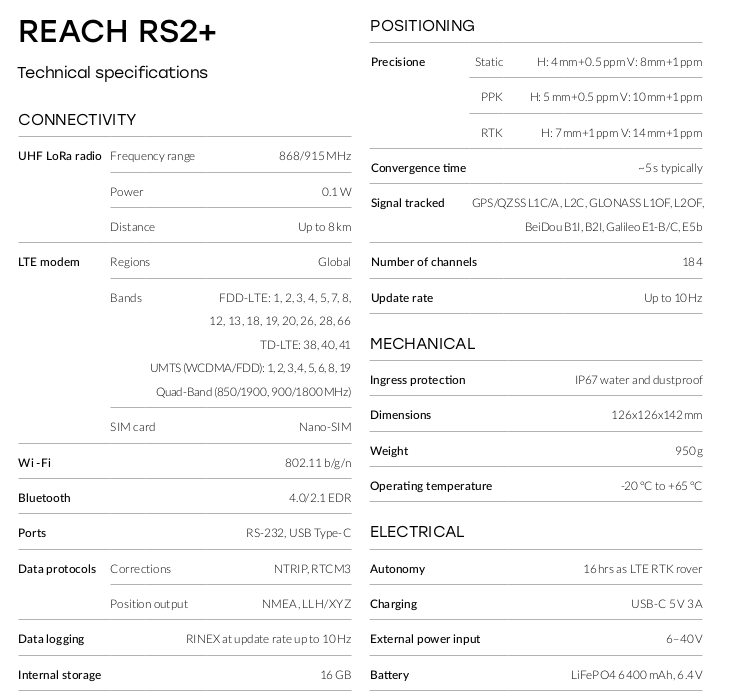
\includegraphics[width=\textwidth]{images/reach_datasheet.png}
    \caption{Hoja de datos del GPS Reach RS2+. Fuente: Emlid}
    \label{fig:datasheet_reach}
  \end{minipage}
\end{figure}



\subsection{IMU Xsens MTi-3th}

El último sensor usado es una IMU de 9 grados de libertad de la marca Xsens (hoy en día conocida por Movella), 
\textbf{figura \ref{fig:xsens_imu}},que cuenta con mágnetometro, \textbf{figura \ref{fig:xsens_datasheet}}. Este dispositivo es antiguo y por tanto 
no existía driver para ROS2, por tanto como paso preliminar se desarrolló un driver para su comunicación. El código de este driver está recopilado junto 
con el resto de algortimos en el repositorio de GitHub creado para este trabajo.

\begin{figure}[!htb]
  \centering
  \begin{minipage}[b]{0.35\textwidth}
    \centering
    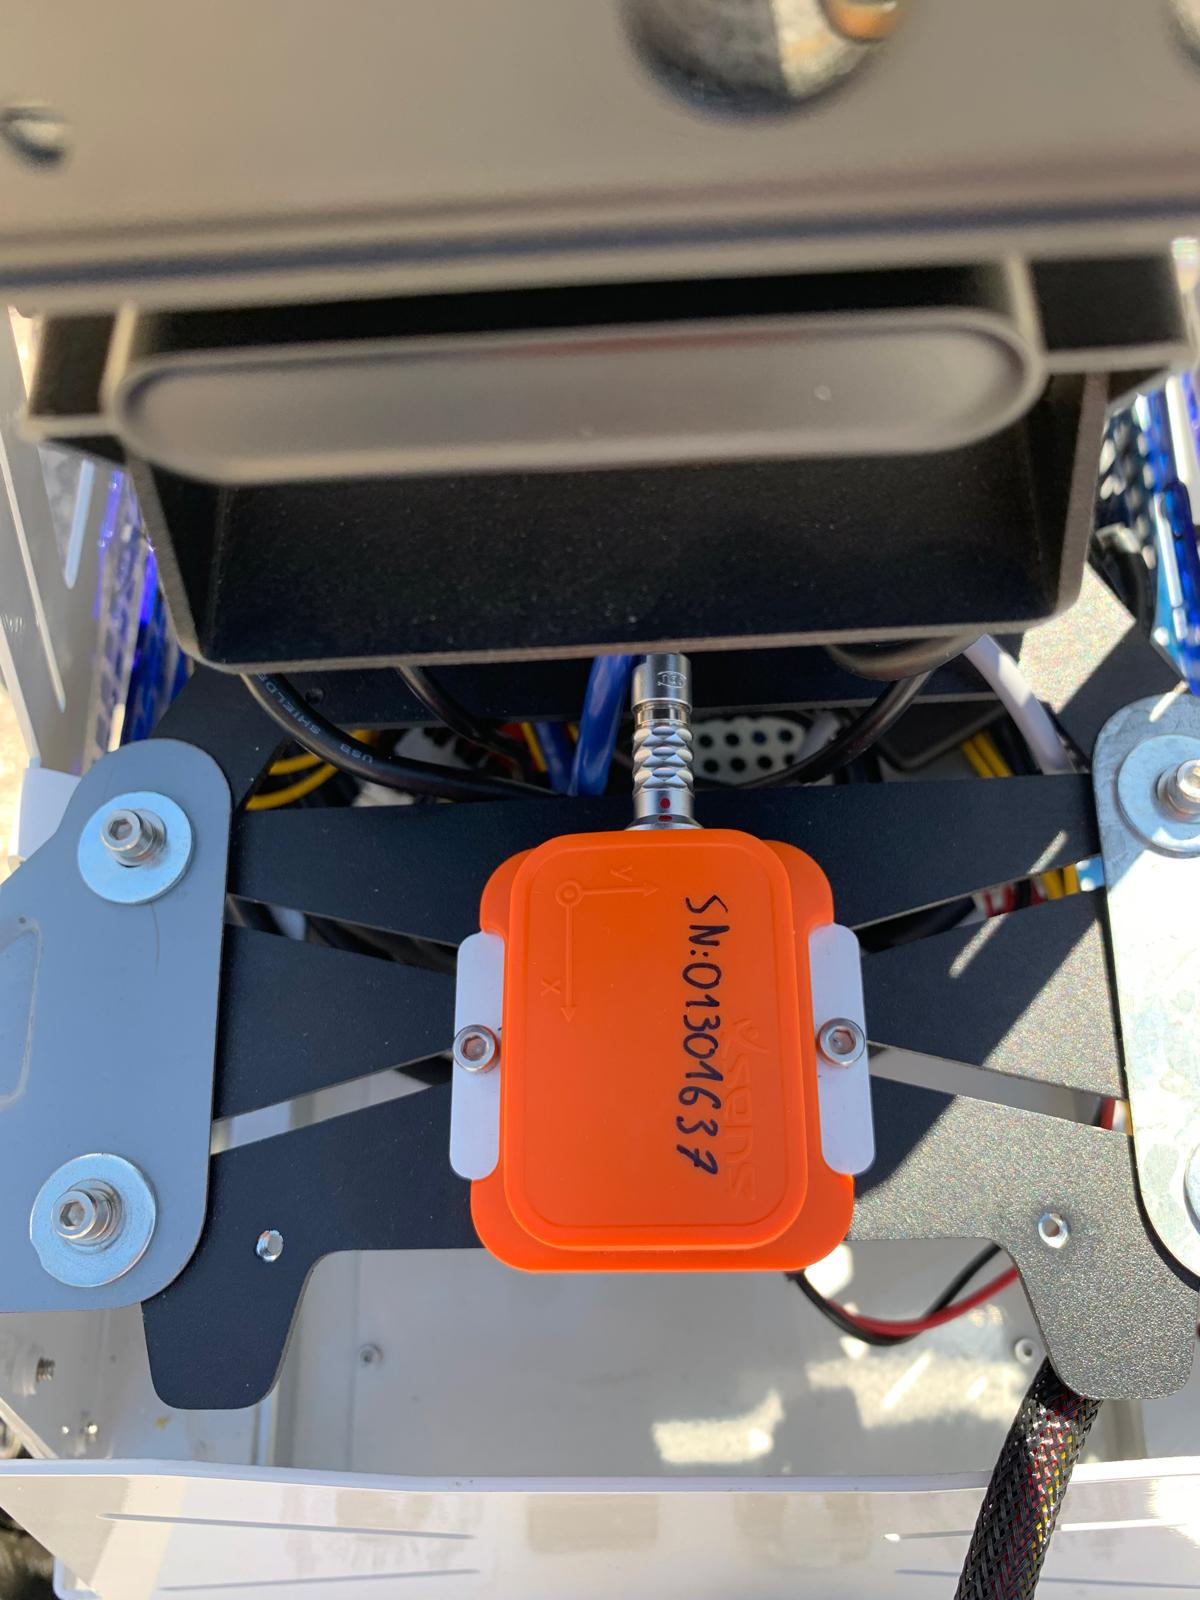
\includegraphics[width=\textwidth]{images/xsens.jpeg}
    \caption{Xsens 3th gen MTI. Fuente: propia}
    \label{fig:xsens_imu}
  \end{minipage}
  \hfill
  \begin{minipage}[b]{0.5\textwidth}
    \centering
    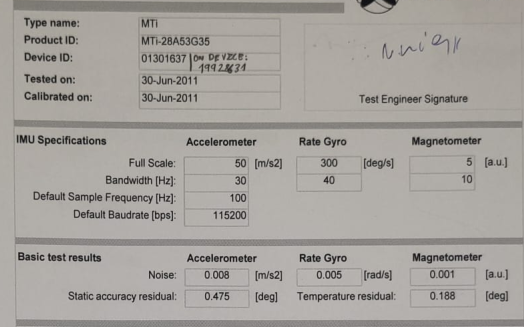
\includegraphics[width=\textwidth]{images/datasheet_mti.png}
    \caption{Hoja de datos de la IMU MTi-3th. Fuente: Xsens}
    \label{fig:xsens_datasheet}
  \end{minipage}
\end{figure}
\newpage
En las \textbf{figuras \ref{fig:mti_velocidad_orientacion} y \ref{fig:mti_aceleraciones}} se puede observar el comportamiento de, por un lado 
la orientación y la velocidad angular en el eje z donde se puede comprobar una salida bastante estable y por otro lado el comportamiento 
de las aceleraciones, en este caso extremadamente ruidoso, también aquí se puede comprobar que la IMU está en el sistema de referencia correcto 
ya que \begin{math}\ddot{Z}\end{math} debe ser positiva y tener de media un valor de aproximadamente 9.81 m/s² que es exactamente lo que se ve. En cuanto a la 
señal ruidosa de aceleraciones se verá más adelante que no es un problema dado que para utilizar esta señal en localización será integrada en el tiempo 
y por tanto simplemente servirá como una redundancia en la odometría de la velocidad lineal.


\begin{figure}[htbp]
  \centering
  \begin{minipage}[b]{0.45\textwidth}
    \centering
    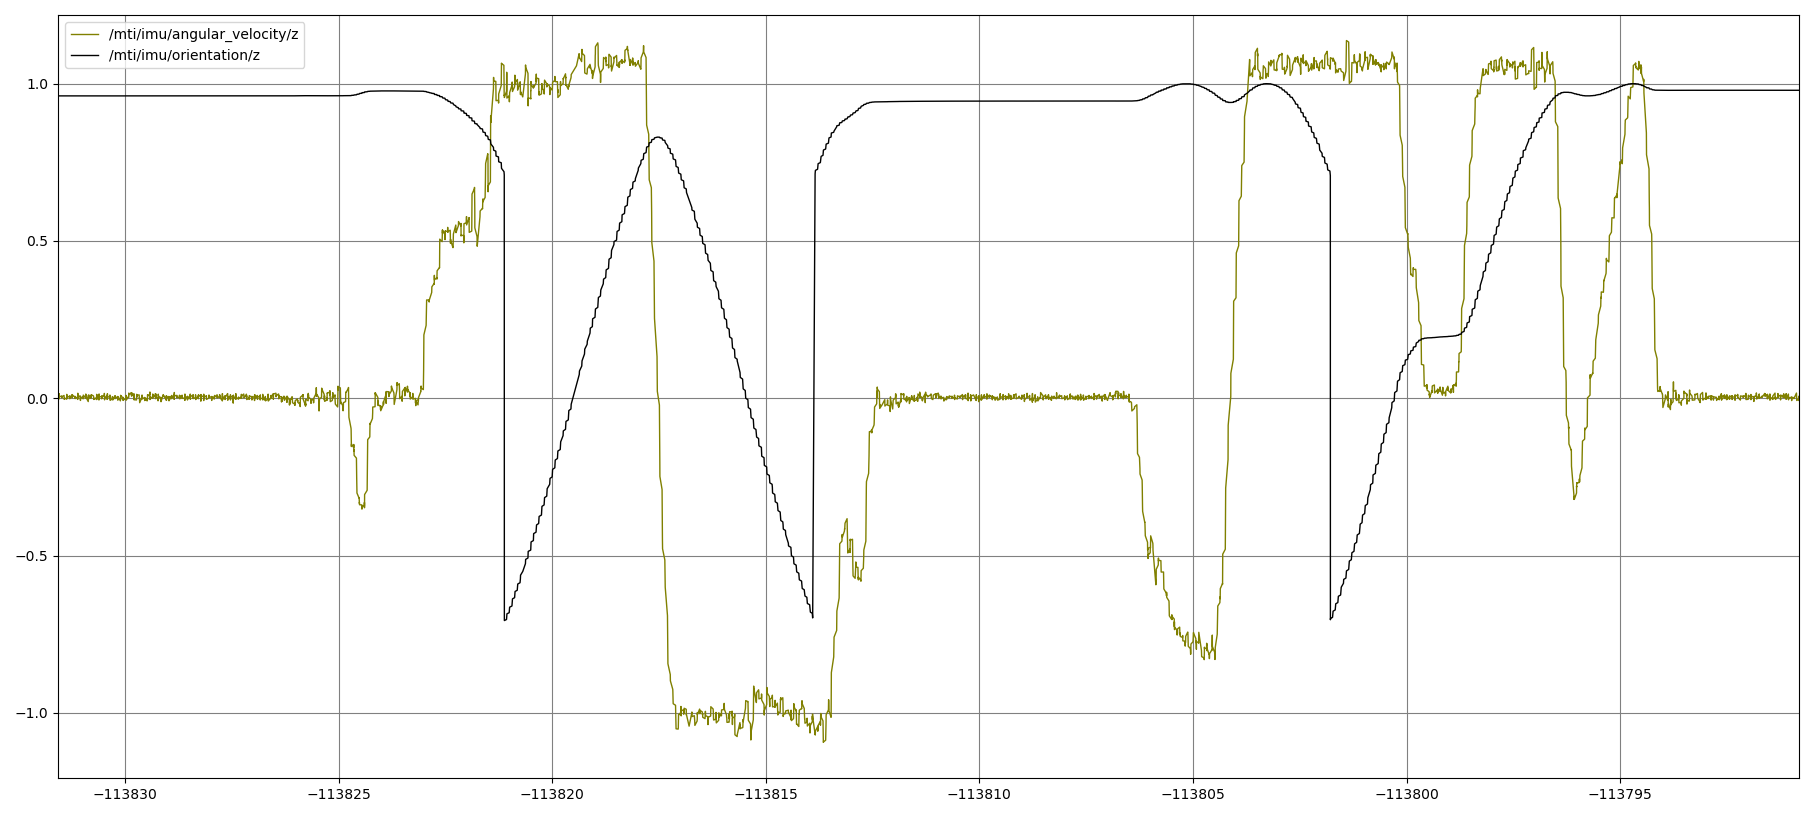
\includegraphics[width=\textwidth]{images/mti_angular_orientation.png}
    \caption{Variaciones de orientación y de velocidad angular en el eje z. Fuente: propia}
    \label{fig:mti_velocidad_orientacion}
  \end{minipage}
  \hfill
  \begin{minipage}[b]{0.45\textwidth}
    \centering
    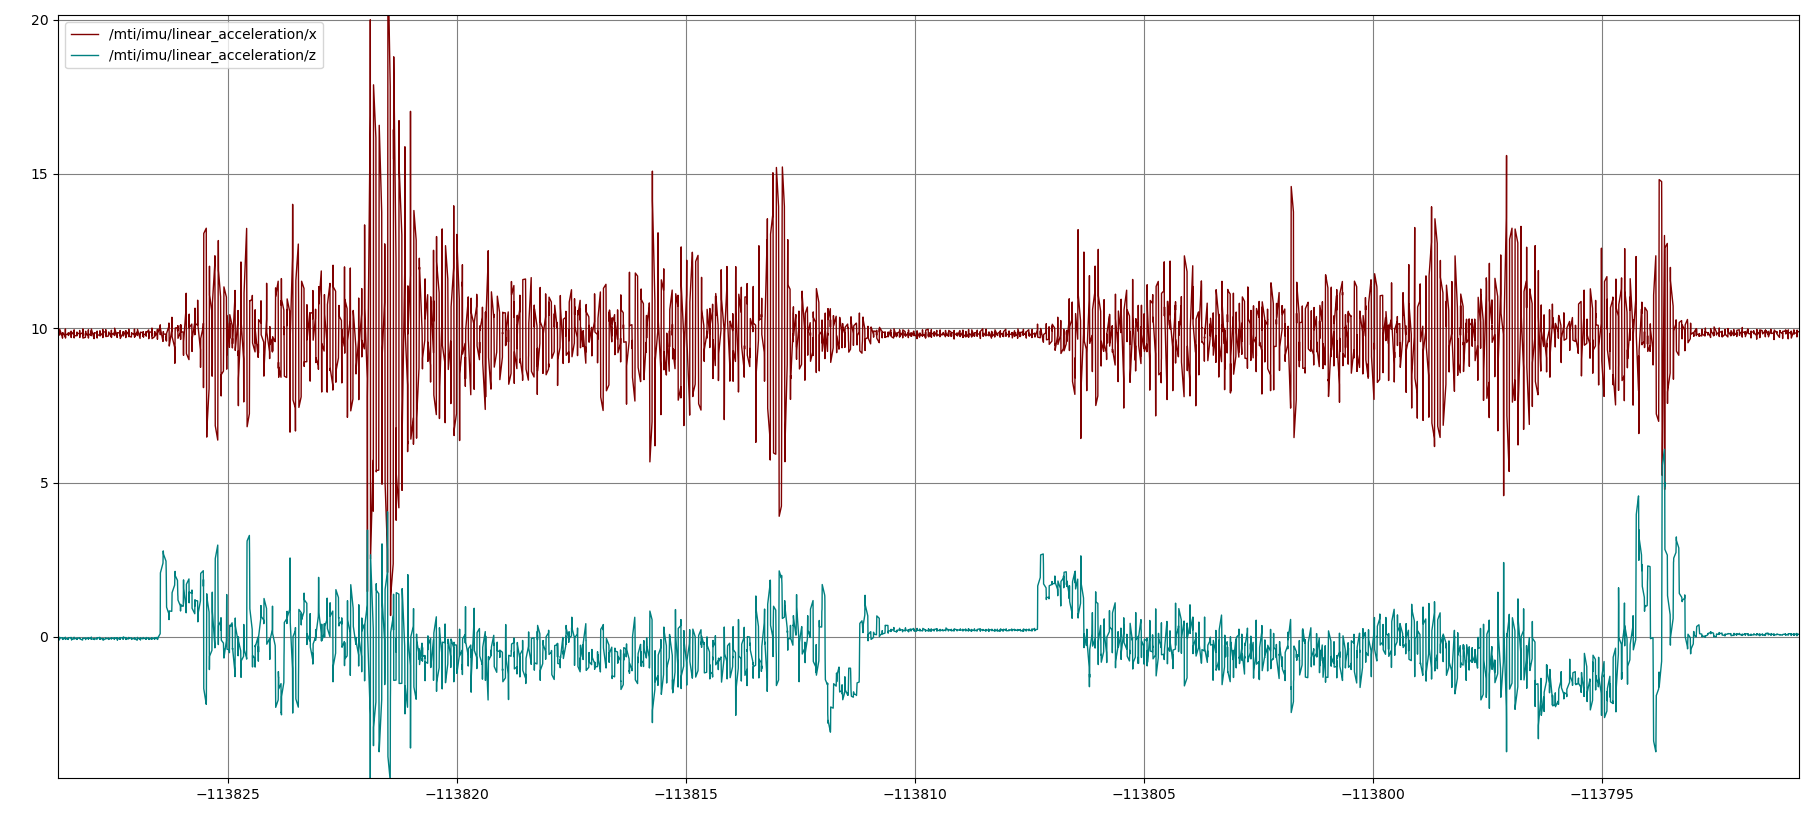
\includegraphics[width=\textwidth]{images/mti_Acceleration.png}
    \caption{Variaciones de aceleración lineal en el eje x y el eje z. Fuente: propia}
    \label{fig:mti_aceleraciones}
  \end{minipage}
\end{figure}

\subsection{Implementación del sistema sensorial en ROS2}

Una vez montados e instalados todos los dispositivos se hicieron pruebas para valorar su efectividad real en el terreno y la configuración 
de los parámetros adecuados para los drivers.

ROS2 funciona con un sistema de descripción cinemática y dinámica escrito en archivos URDF (Unified Robot Description Format), en concreto en 
el lenguaje \textbf{xml} y describe las transformaciones que existen entre los distintos componentes del robot, funciona como un árbol de 
transformaciones donde el elemento base sería el chasis, que según la \textbf{REP 105} (ROS Enhancement Proposal)~\cite{rep105} el nombre para este 
elemento debe ser ''\textit{base\_link}'', está REP describe en detalle las convenciones respecto a nombres para todo el framework de ROS. 

Las transformaciones pueden ser de 2 tipos, estáticas o dinámicas. Las estáticas las compondrían las transformaciones fijas entre los 
sensores y el ''\textit{base\_link}'' y las dinámicas las transformaciones que pueden variar en el tiempo, como el cambio de pose desde 
un instante inicial al actual, el que según la \textbf{REP 105}, se debe llamar \textit{odom}, que viene de odometría en inglés, otro 
ejemplo sería la transformación entre un mapa fijo definido a priori y la posición actual del robot.

Estos 2 flujos de datos son publicados 
por los \textit{topics} \textit{/tf\_static} y \textit{/tf}, respectivamente, para la creación del árbol estático de transformaciones, se 
miden las correspondientes distancias y se definen en un archivo xml como ya se ha comentado, finalmente se publican por los debidos topics. 
Estos árboles de transformaciones pueden contener más información como el tipo de movimiento respecto de el sistema de referencia, 
(fijo, de revolución acotada o de revolución continua), la geometría de los objetos y de sus colisión en el espacio o incluso de sus 
inercias, estas características aunque inútiles para la implementación en un robot real son muy útiles para hacer simulaciones precisas 
en motores de simulación como Gazebo o Coppelia (antiguo V-Rep), las transformaciones dinámicas se calcularán con uno de 
los paquetes usados, \textit{robot\_localization}, del cual se hablará en profundidad más adelante.

En la  \textbf{figura\ref{fig:arbol_urdf}}, se puede observar el árbol completo del robot, desde las transformaciones dinámicas, 
(map, odom y utm) hasta las estáticas (base\_link, gps\_frame, mti\_imu\_frame, etc...)

\begin{figure}[H]
    \centering
    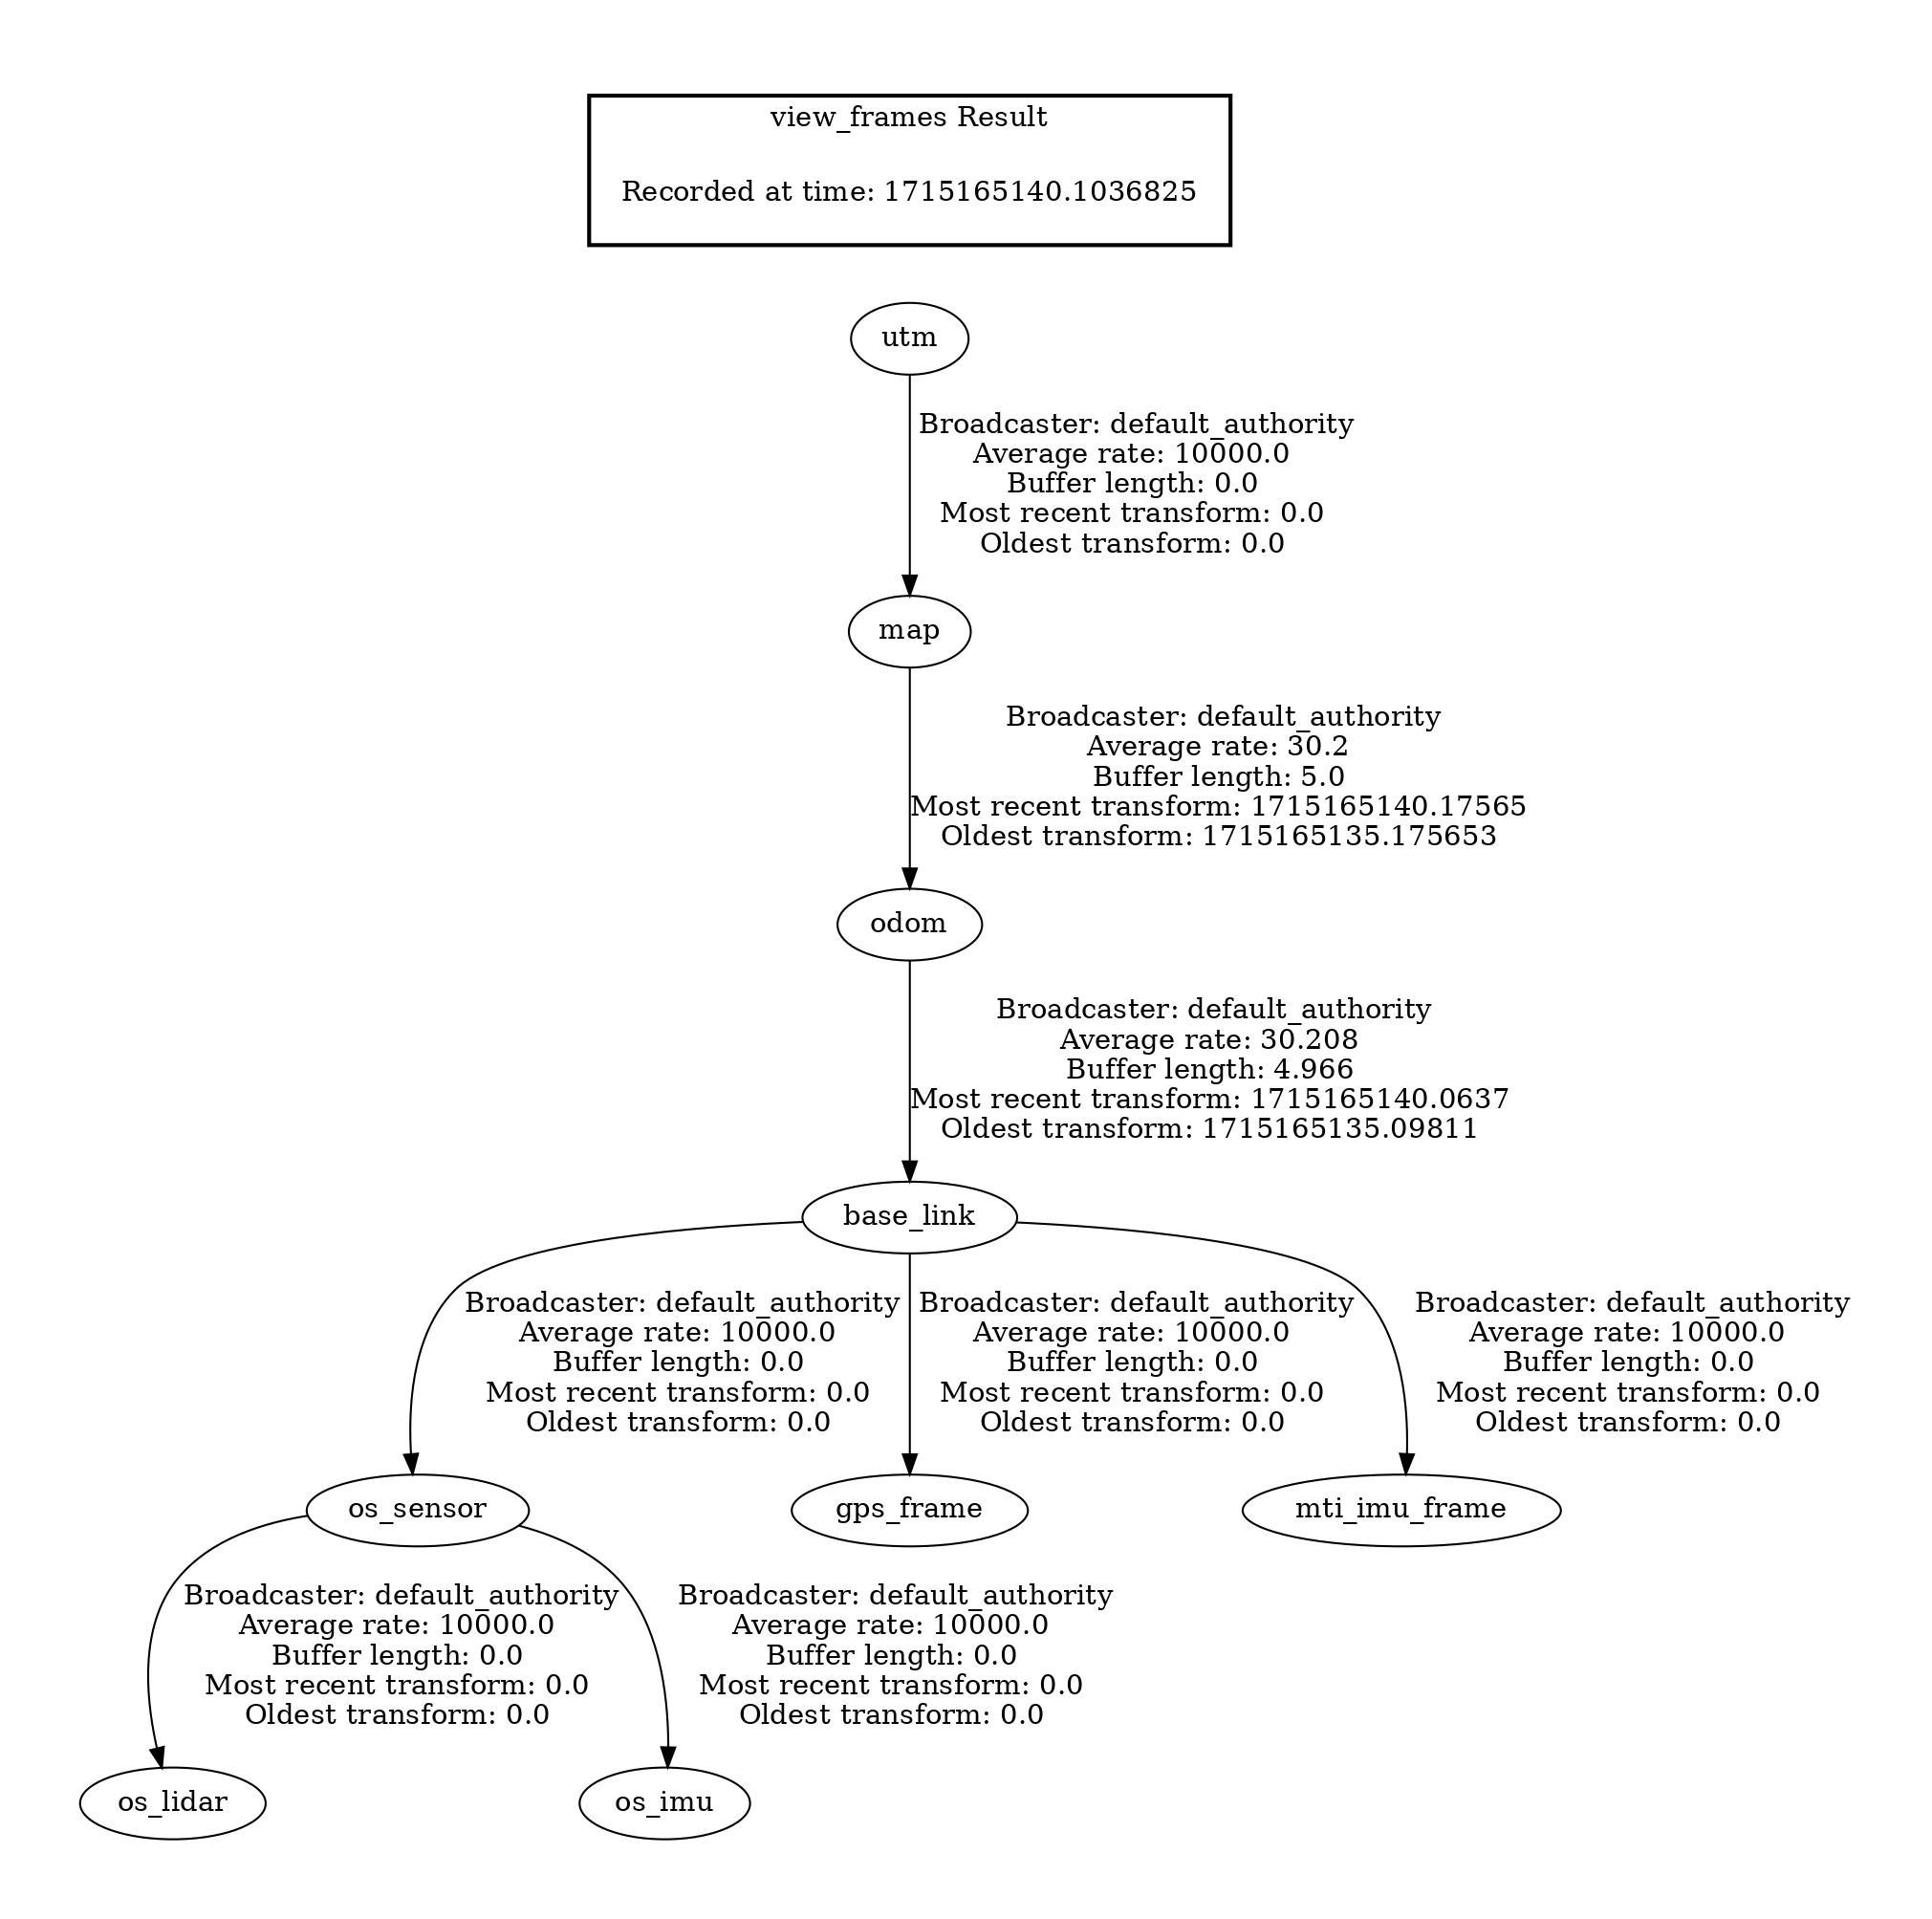
\includegraphics[width=0.6\textwidth]{images/arbol_transformaciones_hunter.jpg}
    \caption{Árbol de transformaciones, Fuente: propia}
    \label{fig:arbol_urdf}
\end{figure}

\newpage
\section{Interfaz de usuario}

Para la creación de la interfaz de usuario se decidió usar \textit{React}, una biblioteca de Javascript de código abierto para la creación de 
interfaces de usuario, por ser una manera relativamente fácil de crear una interfaz web sin tener experiencia en este campo. Para ello 
y según los objetivos se hizo uso de una API de google maps para obtener un mapa junto con las herramientas  
(número 1 de la \textbf{figura \ref{fig:interfaz_1}}), que esta API incluyen, estas son, la posibilidad de mover waypoints y obtener 
las coordenadas GPS del mismo, establecer áreas, tanto rectángulos como polígonos o establecer polilíneas a modo de camino.

Para el protocolo de envío se escogió MQTT, por ser un protocolo rápido y sencillo de implementar, el procedimiento de uso es el que 
sigue, nada más conectarse a la web el protocolo de envío permanece inactivo, no es posible el envío de datos hasta que el usuario pulsa el 
botón de conexión (número 2 de la \textbf{figura \ref{fig:interfaz_1}}) con el broker MQTT, esto esta hecho para cerciorarse de que 
la conexión con el servidor broker se ha establecido correctamente, seguidamente se puede observar como dos botones más se activan~,\textbf{figura \ref{fig:interfaz_2}}, 
uno para publicar y otro para activar la funcionalidad del "follow me", (número 3 y 4 respectivamente en la 
\textbf{ figura \ref{fig:interfaz_2}}).

El ''follow me'' o seguimiento dinámico de personas se describe como un protocolo por el cual el robot es capaz de seguir a una cierta distancia a un individuo, en este caso en base 
a la posición GPS proporcionada por un dispositivo móvil.

FInalmente, para indicar un waypoint al que ir se hace uso del marcador existente en pantalla 
(3 en la \textbf{figura \ref{fig:interfaz_1}}) y para crear un camino formado por múltiples waypoints se hace uso de la paleta de 
herramientas, (2 en la \textbf{figura \ref{fig:interfaz_2}}). Para finalizar, se hace uso del botón "publish" 
(3 en la \textbf{figura \ref{fig:interfaz_1}}), esto esta hecho para que se pueda comprobar que el envío de waypoint o waypointa es correcto antes 
de ser enviado.

\begin{figure}[htbp]
  \centering
  \begin{minipage}[b]{0.45\textwidth}
    \centering
    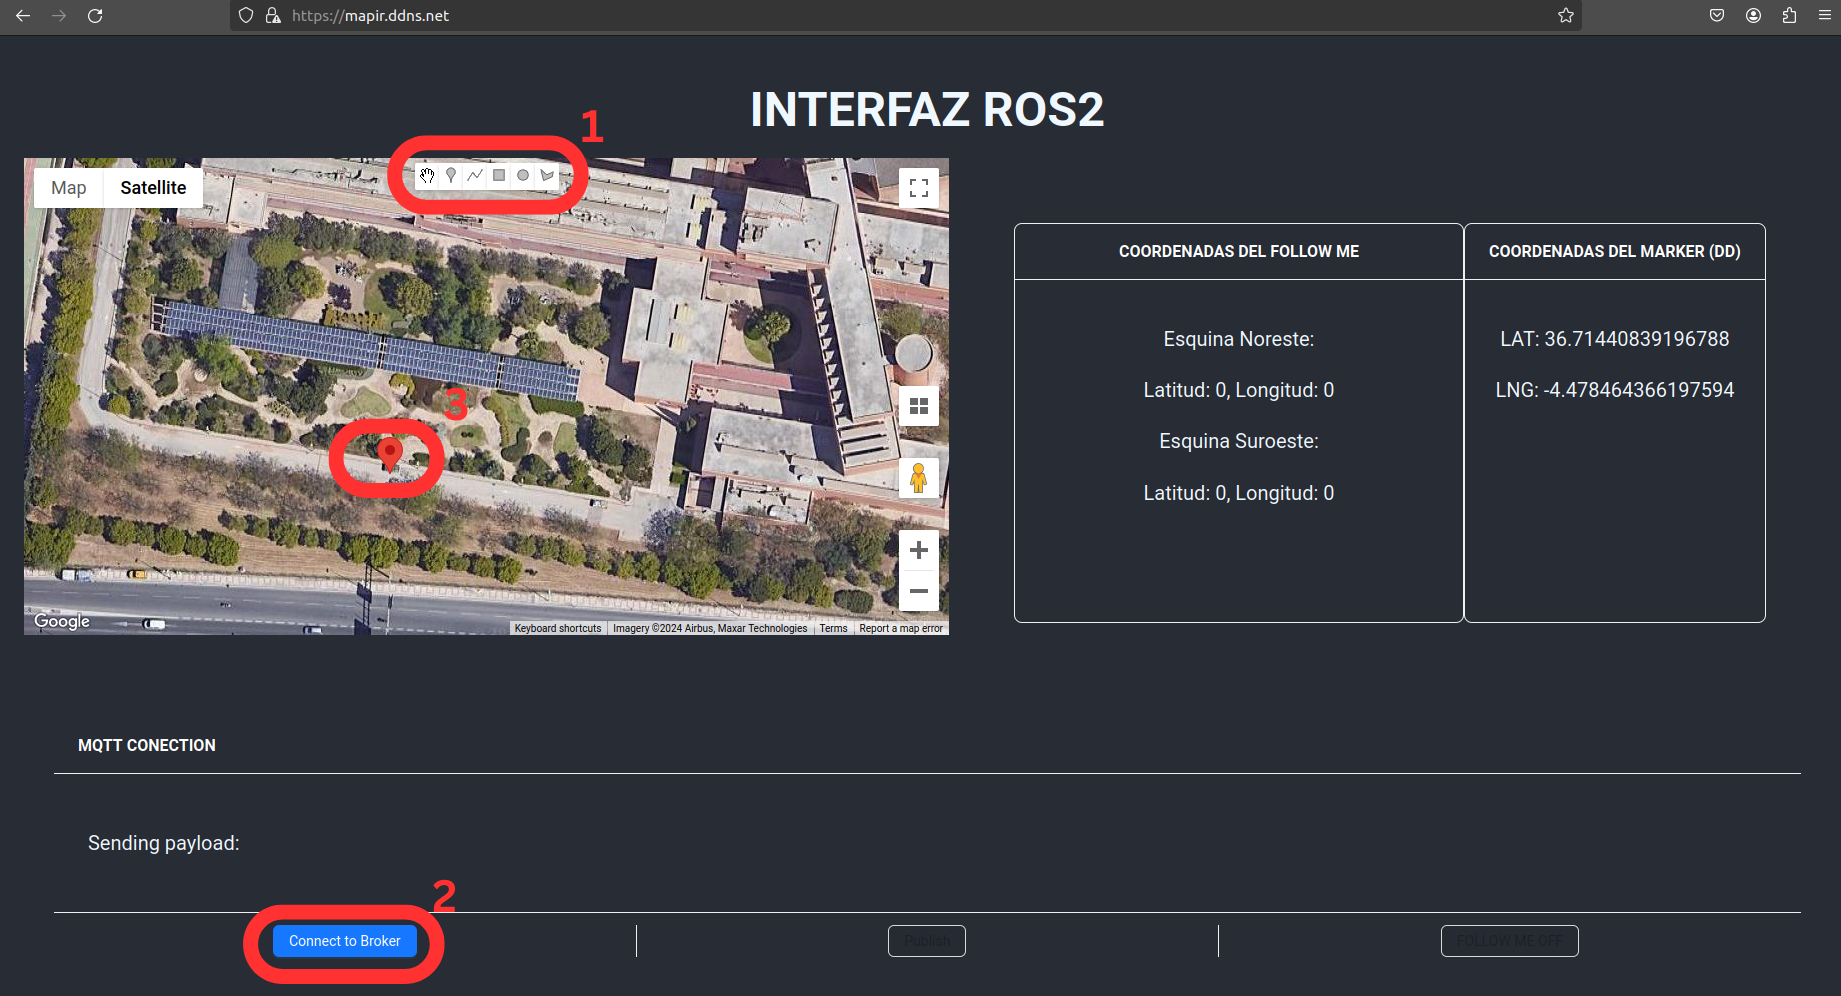
\includegraphics[width=\textwidth]{images/interfaz_1.png}
    \caption{primer estado de la interfaz. Fuente: propia}
    \label{fig:interfaz_1}
  \end{minipage}
  \hfill
  \begin{minipage}[b]{0.45\textwidth}
    \centering
    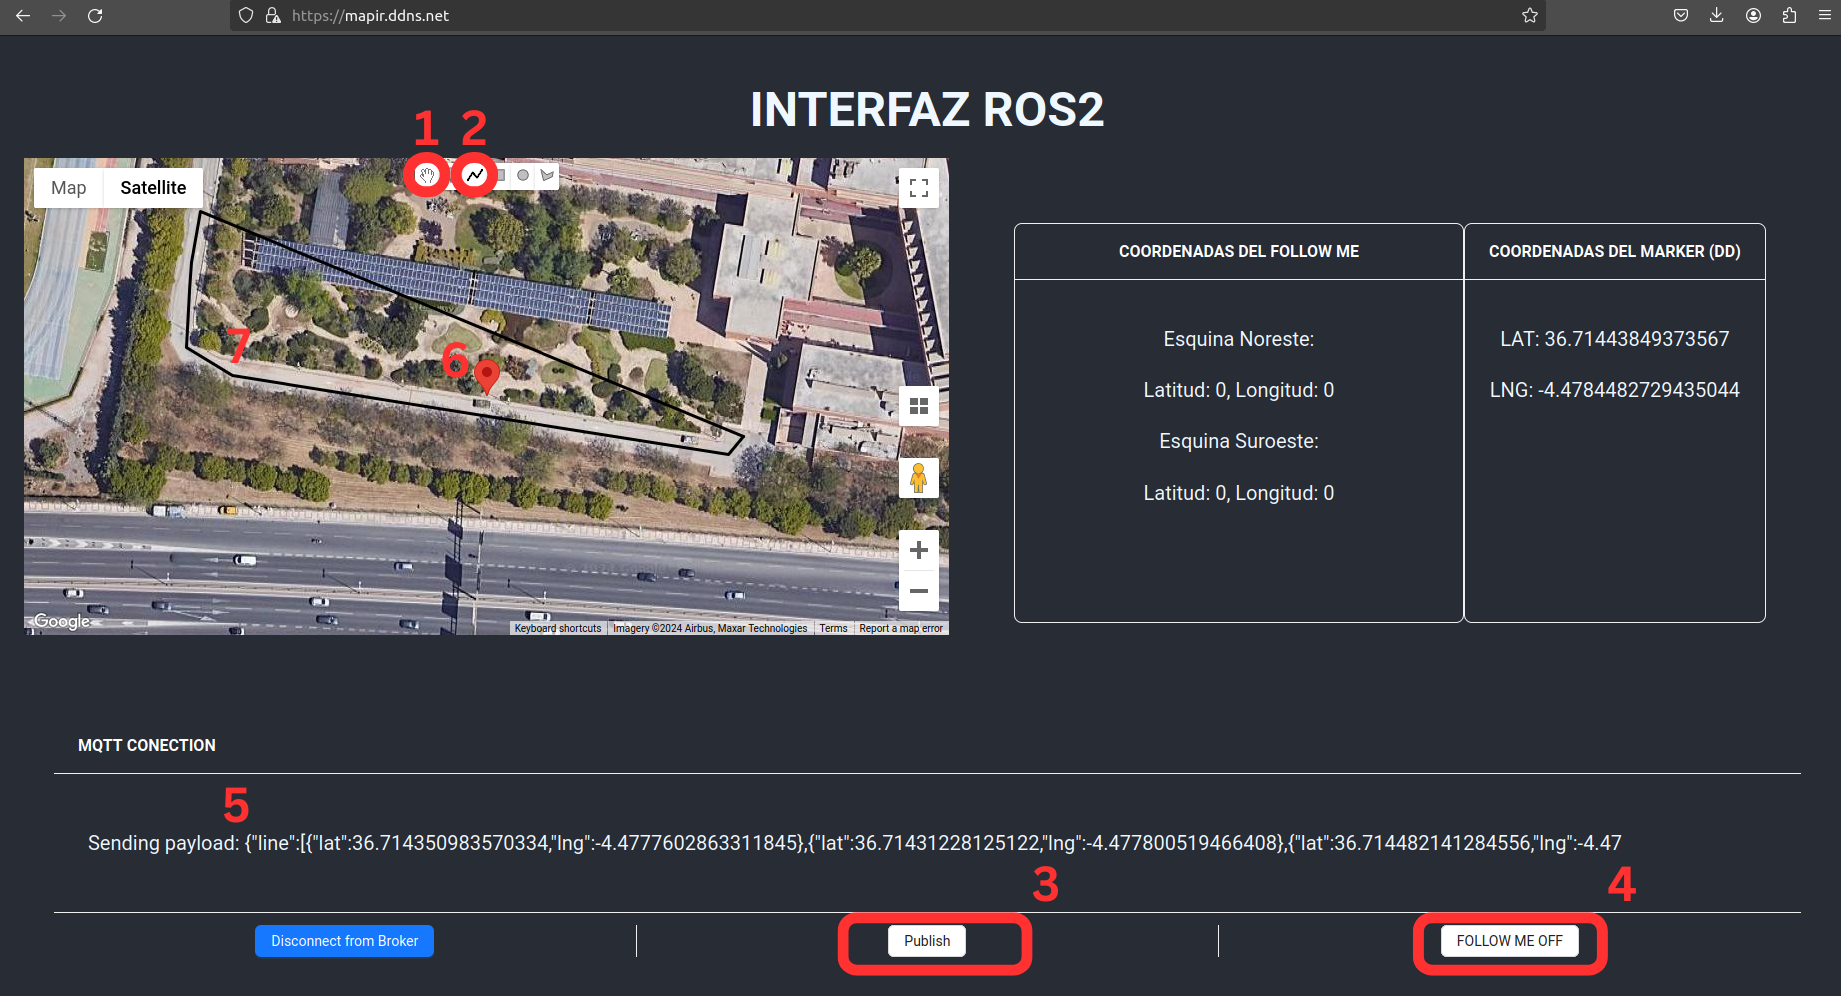
\includegraphics[width=\textwidth]{images/interfaz_2.png}
    \caption{segundo estado de la interfaz. Fuente: propia}
    \label{fig:interfaz_2}
  \end{minipage}
\end{figure}

La aplicación web está alojada en un servidor privado montado en una Raspberry pi 3B+, como software de servidor se ha hecho uso de apache2, 
un servicio de código abierto para implementación de servidores HTTP/1.1 y Mosquito como broker MQTT, ambos instalados y configurados en la propia 
Raspberry. De esta manera se abre la posibilidad de utilizar la página en cualquier lugar del mundo, también, se ha utilizado un servicio de DNS dinámico (DDNS) 
que permite a los usuarios asignar un nombre de dominio a una dirección IP dinámica, NO-ip en nuestro caso, de esta manera en cualquier 
lugar se puede abrir la aplicación y controlar el vehículo de manera visual e intuitiva. Finalmente
comentar que también se desarrollado tanto el envío de areas rectangulares como poligonales, ya que aunque esta 
funcionalidad no se ha implementado en el robot por no ser de interés para el propósito real de este robot, en los objetivos se estableció 
una interfaz ampliable y fácilmente actualizable.


La funcionalidad interna tanto de MQTT como de ROS2 es en base a \textit{topics} o temas por los que se transporta la información, estos 
mensajes forman una cadena desde que se envían en la web hasta que se reciben en el ROS2.

Como se puede ver en el \textbf{esquema \ref{fig:esquema_flujo_datos}} se han implementado 3 topics, el primero y más importante 
\textit{/desired\_pos}, por donde se envían las coordenadas del objetivo u objetivos, este mensaje formateado en JSON contiene principalmente 2 
campos, el primero es el tipo que puede ser, ''marker'', ''line'', ''rectangle'', ''polygon'' o ''follow'' y el segundo campo contiene o 
una tupla con la latitud y longitud del objetivo o un array de tuplas para los casos más complejos, el topic \textit{/follow} es una \textit{flag}, 
es decir un valor booleano para saber si el ''follow me'' está activado o no, el tercero es un mensaje al que se subscribe el servidor web con 
la información de la posición actual del robot.

Se ha hablado de la implementación de la interfaz y de su envío mediante un broker hasta el robot pero no de como se recibe esta información 
y se transforma a un mensaje útil para el entorno de desarrollo usado (ROS2), al enviar los mensajes formateados en JSON 
se deberán convertir en tipo \textit{string}. En caso contrario, nuestro receptor no los entenderá. Este es un nodo, (MQTT Bridge), que se conecta con el broker 
establecido, se subscribe a los topics que se requieren y los transforma a un tipo de dato que ROS2 entiende, este es también un tipo \textit{string} pero propio 
de ROS2, por tanto para obtener la información necesaria se deberá \textit{parsear} ese mensaje transformándolo de un string de vuelta a una 
tupla de coordenadas o a un string de tuplas de coordenadas.
\begin{figure}[h]
\begin{center}
\begin{tikzpicture}[scale=1, node distance=2.5cm,>=Latex, mynode/.style={draw, rectangle, rounded corners=5pt}]
    % Definir nodos
    \node [mynode] (webserver) {WEB};
    \node [mynode, right=of webserver] (mqttbroker) {MQTT BROKER};
    \node [mynode, right=of mqttbroker] (mqttbridge) {MQTT BRIDGE};
    \node [mynode, right=of mqttbridge] (rosframework) {ROS2};
    
    % Dibujar líneas hacia adelante con nombre
    \draw[->] (webserver) -- (mqttbroker) node[midway, above] {/follow};
    \draw[->] (mqttbroker) -- (mqttbridge) node[midway, above] {/follow};
    \draw[->] (mqttbridge) -- (rosframework) node[midway, above] {/web/follow};
    \draw[->, bend left] (webserver) to node[midway, above] {/desired\_pos} (mqttbroker);
    \draw[->, bend left] (mqttbroker) to node[midway, above] {/desired\_pos} (mqttbridge);
    \draw[->, bend left] (mqttbridge) to node[midway, above] {/web/desired\_pos} (rosframework);
    
    % Dibujar línea hacia atrás con nombre
    \draw[->,red, bend left] (mqttbroker) to node[midway, below] {/position} (webserver);
    \draw[->,red, bend left] (mqttbridge) to node[midway, below] {/position} (mqttbroker);
    \draw[->,red, bend left] (rosframework) to node[midway, below] {/web/gt} (mqttbridge);
\hfill{}

\end{tikzpicture}
\end{center}
\caption{Esquema de flujo de datos desde la Web hasta ROS2}
\label{fig:esquema_flujo_datos}
\end{figure}

Para ello se creó un nodo que recibe la información del nodo MQTT Bridge y 
lo \textit{parsea} haciendo uso de la librería \textit{jsoncpp}, primero se lee el campo qué nos indica que tipo de mensaje es, es 
decir si es un marcador o es un conjunto de ellos, seguidamente lo guardamos en una variable con un tipo de dato personalizado, para los 
marcadores el tipo de datos contiene un campo para longitud y otro para latitud y para los caminos o conjunto de objetivos, contiene \textit{array} de marcadores y un entero 
para indicar el tamaño, de esta manera se hace más sencillo el procesamiento de los mismos.


\newpage
\section{Procesamiento de los mensajes MQTT a ROS2}
Por razones que se entenderán más avanzado el capítulo estos datos se deberán procesar todavía más, primero haciendo uso de un servicio de ROS2 
implementado por el paquete \textit{robot localization} que transforma las coordenadas GPS expresadas en ángulos a un sistema cartesiano 
centrado en el punto de inicio de movimiento del robot y después se deberá comprobar la distancia desde la posición actual del robot al punto que se desea alcanzar.

Esto es debido a la manera en la que Nav2 funciona, si la distancia es menor a un valor dictado por los parámetros de Nav2 se podrá enviar directamente 
al siguiente nodo, de no ser así se generarán puntos equiespaciados desde la posición del robot hasta el objetivo y posteriormente se enviará ese \textit{array} 
de posiciones, cabe destacar que se deberá generar la orientación deseada, cosa que la web no proporciona.

Para ello simplemente se calculará el ángulo que existe entre la posición del robot y la de el objetivo, para el caso de tener varios objetivos contiguos, es decir una 
ruta o camino se hace este mismo algoritmo por cada par de puntos. El pseudo código se proporciona en el \textbf{algoritmo \ref{objetivos}}.

\begin{algorithm}[H]
  \caption{Procesamiento de objetivos}\label{objetivos}
  \begin{algorithmic}[1]
    \Procedure{Procesamiento}{JSONmsg} \Comment{Cálculo final de trayectoria genérica}
        \State $tipo\gets JSON.parse(JSONmsg)["type"]$
        \If{$tipo="marker" || tipo="follow"$}  
       
            \State $objetivo\gets JSON.parse(JSONmsg)["coordinates"]$
             \If{$dist(robot.position, objetivo) > rango $}
                \State $array\_objetivos \gets puntos\_intermedios(robot.position, objetivo, rango)$ 
                \State $publish(array\_objetivos)$
             \Else
                \State $publish(objetivo)$
             \EndIf
        \Else
            \For{$p \gets objetivos$} \Comment{Se hace el mismo algortimo por cada 2 puntos del array}
                \If{$dist(p_0, p_1) > rango $}
                \State $array\_objetivos.push\_back( puntos\_intermedios(p_0, p_1, rango))$
             \Else
                \State $array\_objetivos.push\_back(objetivo)$
             \EndIf
            \EndFor
            \State $publish(array\_objetivos)$
        \EndIf
    \EndProcedure
  \end{algorithmic}
\end{algorithm}

Una vez procesada la información obtenida de la Web, se publicará hacia otro nodo encargado de la lógica de control del paquete de 
navegación, este indicará a Nav2 donde ir y como ir, pero antes de ello se deberá conseguir una localización estable en el tiempo.

\section{Localización y odometría}

La localización en robótica es uno de los problemas más explorados dada su importancia, por ello esta parte posiblemente sea la más 
importante del proyecto y la que más tiempo llevo conseguir.

Primero se investigaron las mejores estrategias para conseguir una buena localización en exteriores, donde a diferencia de los espacios interiores 
esta tarea se vuelve un considerablemente más compleja. Existen métodos como SLAM o AMCL que funcionan muy bien en interiores pero en 
ambientes tan cambiantes y con tan pocas referencias estas alternativas se vuelven totalmente 
inservibles.
Principalmente se tienen 2 fuentes de odometría (IMU, Encoders de las ruedas) y 1 fuente de localización (GPS), existen múltiples 
opciones para conseguir una buena localización en base a estos dispositivos 
pero la más usada es sin duda lautilización de filtros extendidos de \textbf{Kalman} para fusionar múltiples fuentes de odometría. 
 
El \textbf{GNSS} (Global Navigation Satellite System) es una tecnología que funciona en base a una triangulación con satélites que 
estén a ''la vista'' en ese momento, normalmente esta 
posición es calculada por medio del estándar \textbf{WGS84}, siendo este el estándar más reciente creado para este propósito. A 
diferencia de muchos de sus antecesores este modelo tiene en consideración 
que la tierra es elíptica y no totalmente esférica. En la \textbf{figura \ref{fig:wgs84}} podemos ver el modelo WGS84 y sus sistema 
de referencia, el cual encontraríamos en el centro de la tierra 
con su eje \textbf{z} apuntando al Norte y su eje \textbf{x} apuntando al primer meridiano.

\begin{figure}[h]
    \centering
    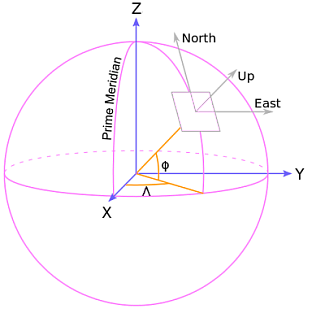
\includegraphics[width=0.46\textwidth]{images/wgs84.png}
    \caption{Sistema de referencia del modelo WGS84. Fuente: \cite{nav2}}
    \label{fig:wgs84}
\end{figure}

El principal problema de este sistema de referencia es que es bastante impráctico para la aplicación que aquí se discute, por ello,  
se requiere de una transformación a un sistema cartesiano y para ello se debe hablar también del sistema de coordenadas plano \textbf{UTM} 
(Universal Transverse Mercator), un sistema en base a la proyección de Mercator normal, pero en vez de hacerla tangente al Ecuador, 
se la hace secante a un meridiano y esta formado por 60 zonas que dividen el globo entero. En la \textbf{figura \ref{fig:utm_europa}} se 
pueden observar tanto la nomenclatura de cada zona como su disposición.

\begin{figure}[h]
    \centering
    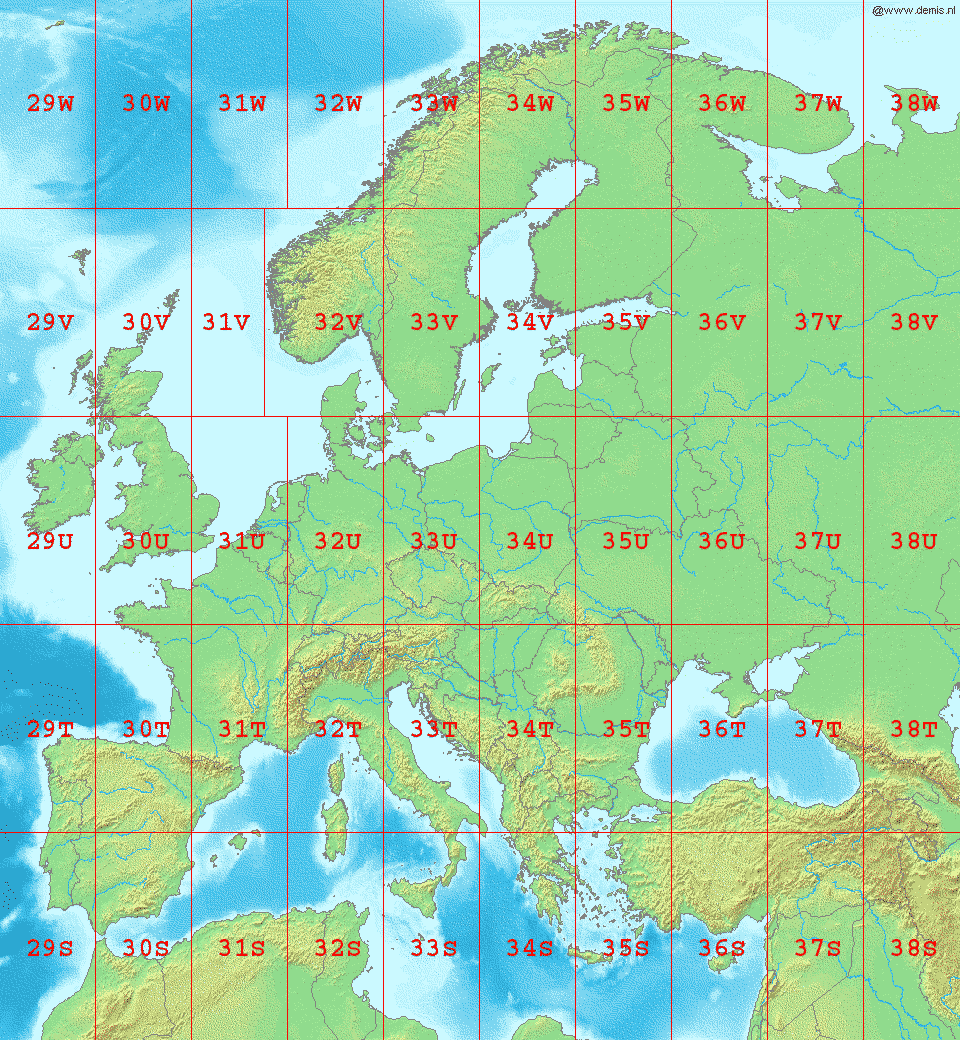
\includegraphics[width=0.5\textwidth]{images/europe_utm.png}
    \caption{Sistema de referencia del modelo UTM en Europa. Fuente: Wikipedia}
    \label{fig:utm_europa}
\end{figure}


A diferencia de las coordenadas geográficas este sistema se expresa en metros lo que ya da una ventaja en cuanto a esta aplicación pero 
sigue habiendo el problema de que estas zonas son demasiado grandes, por lo que también se necesita calcular el \textit{offset} desde el 
origen de una de estas zonas a donde se inicie el robot, nos referiremos a este offset como \textit{Datum}.

Como se puede observar en la \textbf{figura \ref{fig:datum}} a parte de conocer la posición, también se requiere del ángulo o \textit{bearing} 
y la declinación magnética, esta última es la que menos preocupa, dado que es un dato bastante constante en el tiempo y varía por 
zona geográfica (varía alrededor de 0,035 radianes cada 100 años), para el caso de Málaga es igual a 0,061 rad.



\begin{figure}[h]
    \centering
    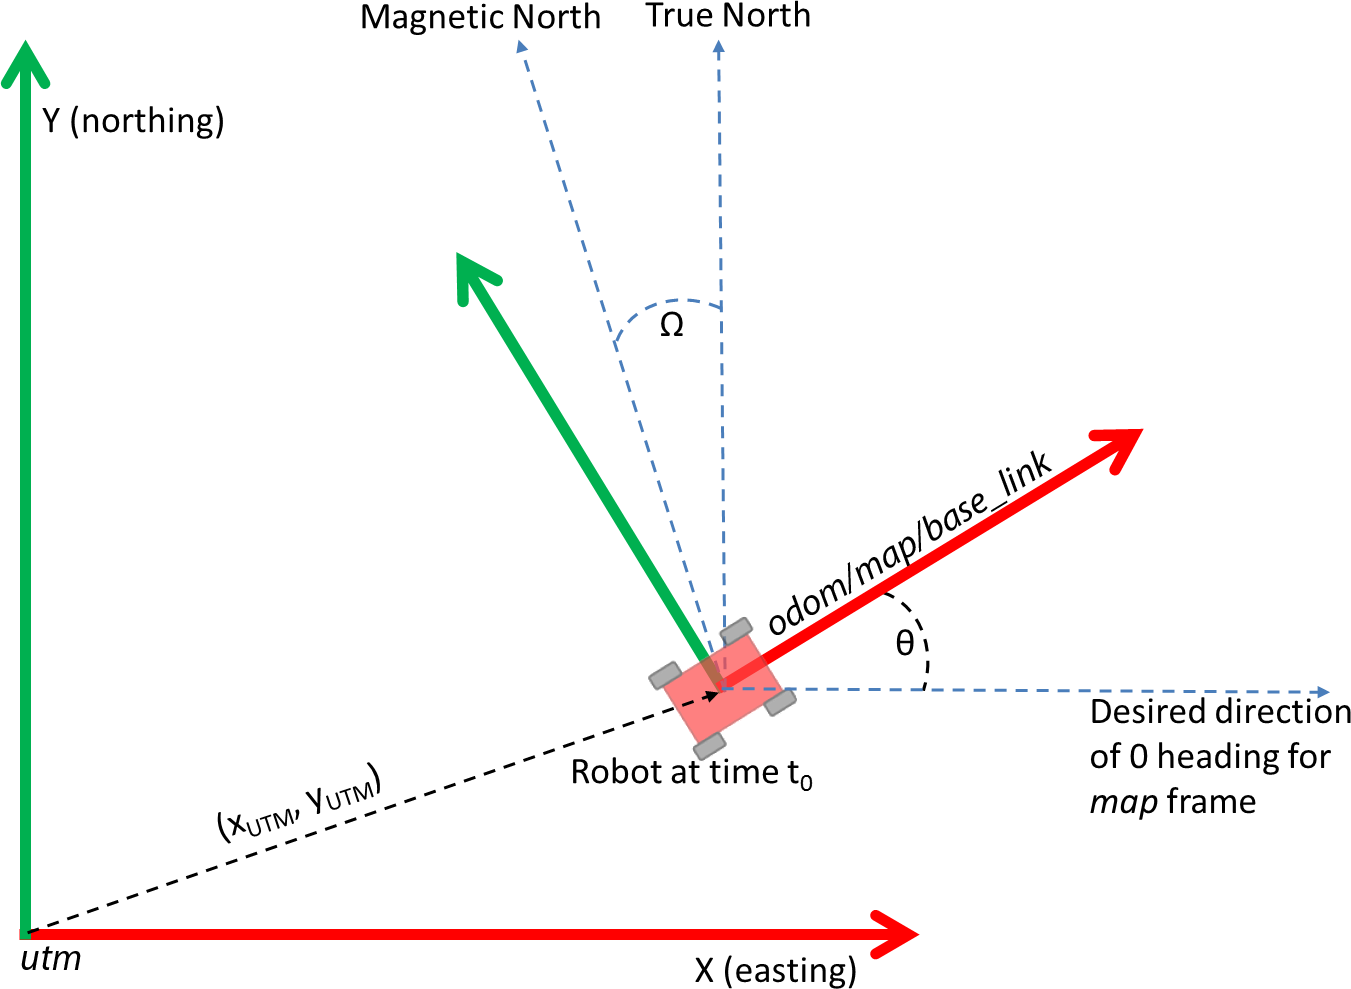
\includegraphics[width=0.65\textwidth]{images/navsat_transform.png}
    \caption{Sistema de referencia Datum. Fuente: \cite{nav2}}
    \label{fig:datum}
\end{figure}

Finalmente se cuenta con el paquete \textit{robot localization} ya comentado, que 
ofrece una manera robusta de transformar los mensajes del GPS expresados en latitud y longitud (altitud se tomará igual a 0) a un 
sistema de referencia cartesiano, el nodo para esta tarea será \textit{navsat\_transform} y básicamente se subscribirá a 3 topics para calcular 
el \textit{Datum} lo que hará una sola vez, para después en lo que se podría llamar el funcionamiento normal del nodo, publicará un mensaje de tipo 
\textit{nav\_msgs/Odometry} que será la transformación del GPS al sistema de coordenadas cartesianas. Para entender mejor el flujo de datos se incluye 
un esquema en la \textbf{figura \ref{fig:esquema_navsat}} y una explicación de las 3 suscripciones que necesitan para trabajar.

\begin{itemize}
    \item Un mensaje de tipo \textit{sensor\_msgs/NavSatFix} con los datos provenientes del GPS, este será \textit{/hunter/fix}
    \item Un mensaje de tipo \textit{nav\_msgs/Odometry} con la posición actual del robot y opcionalmente la orientación, está odometría 
será la salida de uno de los filtros de Kalman, esta información es necesaria en el caso de que 
el primer mensaje de GPS llegue después de que el robot haya empezado a moverse, este será \textit{/odometry/global}.
    \item Para este tercer mensaje se tiene que proporcionar la orientación global respecto al norte magnético y debe usarse la 
convención ENU (East, North, Up), que estipula un sistema de referencia con el Este en el eje \textbf{x} y el Norte en el eje \textbf{y} 
como se puede observar en la \textbf{figura \ref{fig:wgs84}}. Para ello el nodo ofrece 4 maneras de hacerlo, la primera ya ha sido 
comentada y es usando la parte de orientación del primer mensaje de odometría y los otros 3 se listan a continuación.
        \begin{itemize}
            \item Una suscripción a un topic de tipo \textit{sensor\_msgs/Imu} con 9 grados de libertad, (ya que sin ellos no tenemos una 
orientación global respecto al norte magnético).
            \item Utilizar uno de los servicios que ofrece el paquete para que de manera externa ese datum sea calculado y enviado, 
este servicio es \textit{/datum}.
            \item Indicarlo manualmente por medio de un archivo de parámetros en formato \textit{YAML}.
        \end{itemize}
\end{itemize}



\begin{figure}[h]
    

\begin{center}
\begin{tikzpicture}[scale=1.4, node distance=3cm,>=Latex, mynode/.style={draw, rectangle, rounded corners=5pt}]

    \node [mynode] (navsat) {NavSatTransform Node};
    \node [mynode, above= of navsat, xshift = 3cm] (gps) {GPS};
    \node [mynode, above= of navsat, xshift = -3cm] (ekf) {EKF};
    \node [mynode, left=of navsat] (orient) {Método de orientación};
    \draw[->] (orient) -- (navsat) node[midway, above] {orientación};

    \draw[->, bend left] (gps) to node[pos=0.7, below right,rotate=60] {/hunter/fix} (navsat);
    \draw[->, bend right] (ekf) to node[pos=0.8, below left, rotate=-40] {/odometry/global} (navsat);
    
    \draw[->,red, bend right] (navsat) to node[pos=0.8, above right, rotate=-40] {/odometry/gps} (ekf);

\hfill{}

\end{tikzpicture}
\caption{Esquema de flujo de topics en el nodo navsat\_transform}
\label{fig:esquema_navsat}
\end{center}
\end{figure}

Al comienzo del proyecto como ya se ha comentado no se disponía de una IMU con orientación global por lo que se desarrolló un nodo que 
entre otras cosas calcula el ángulo respecto al norte magnético y lo transforma al sistema ENU antes de enviarlo por medio del servicio que \textit{robot\_localization} proporciona.
Para realizar este cálculo primero el nodo se suscribe al topic \textit{/hunter/fix} para obtener así las coordenadas GPS y al topic 
\textit{/hunter/odom} de tipo \textit{nav\_msgs/Odometry} para recibir la información del movimiento del robot, también, publicará por el topic 
\textit{/cmd\_vel} para hacer mover al robot. El procedimiento es el que sigue.

Primeramente se permanece a la espera de la llegada de un mensaje de GPS y se guardan esas coordenadas, posteriormente se hace mover al vehículo una 
determinada distancia hacia delante, es decir solo en el eje \textbf{x} que será 
especificada por el usuario, finalmente sevolverá a esperar a otro mensaje del GPS. Por tanto para la parte de posición se tomará el segundo 
dato de GPS y para el cálculo de la orientación global, denotada como bearing o azimut se seguirán las siguientes ecuaciones que describen el cálculo del rumbo (bearing) entre dos puntos geográficos, dados por sus coordenadas de 
latitud (\(\phi_1, \phi_2\)) y longitud (\(\lambda_1, \lambda_2\)):


\begin{equation}\label{eq:delta_longitud}
\Delta{l} =( \lambda_{2} - \lambda_{1} ) * (\pi/180) 
\end{equation}
\begin{equation}\label{eq:calculo_x}
X = cos(\phi_{2}) * sin(\Delta{l}), 
\end{equation}
\begin{equation}\label{eq:calculo_y}
Y = cos(\phi_{1}) * sin(\phi_{2}) - sin(\phi_{1}) * cos(\phi_{2}) * cos(\Delta{l})
\end{equation}
\begin{equation}\label{eq:calculo_bearing}
bearing = (\pi/2) - fmod((atan2(Y,X) + 2\pi),2\pi)
\end{equation}

Donde:
\begin{itemize}
    \item \(\Delta{l}\) es el cambio en longitud, medida en radianes.
    \item \(X\) es una componente del cálculo intermedio.
    \item \(Y\) es otra componente del cálculo intermedio.
    \item \({bearing}\) es el rumbo entre los dos puntos, medido en radianes.
\end{itemize}

En la \textbf{ecuación \ref{eq:calculo_bearing}}, se puede observar el uso del módulo del ángulo respecto a 360º, esto es debido 
a que la función \textit{atan2} devuelve un valor en el rango $[ -\pi/2,\pi/2 ]$, y en cambio se necesita en
el rango $[0, 2\pi]$, también como se ha comentado este ángulo debe estar acorde al sistema ENU y por tanto se le resta $\pi/2$ para que esto se cumpla. Finalmente 
se enviará al servicio y el nodo  \textit{navsat\_transform}comenzará a funcionar.

Por último falta la configuración de los EKF, para esta implementación se tomará también el mismo paquete que nos ofrece la posibilidad de 
configurarlos de una manera sencilla.

El principal problema que se considera aquí es la diferencia entre la odometría y la localización, donde la primera es muy rápida, 
(más de 30 Hz) y precisa para intervalos de tiempo cortos, es decir acumula error con el tiempo. Por otro
lado la localización proporcionada por el GPS es muy lenta y por tanto discreta, po esta razón no vale para usar en 
intervalos cortos de tiempo pero es extremadamente precisa a la larga ya que es una fuente de posición que por definición no tiene
\textit{deriva} en el tiempo, concluyendo, se necesitarán las dos para conseguir una buena localización.

Para ello se empezará creando una instancia de un filtro de Kalman para las fuentes continuas (Odometrías), este se llamará 
\textit{ekf\_local} ya que se usará para navegación y planificación de movimientos en el sistema de referencia \textit{/odom}, estos 
filtros funcionan con matrices de 15 variables para cada fuente de odometría, estás son: 
$$[ X,Y,Z,\theta_{x},\theta_{y},\theta_{z},\dot{X},\dot{Y},\dot{Z},\dot{\theta_{x}},\dot{\theta_{y}},\dot{\theta_{z}},\ddot{X},\ddot{Y},\ddot{Z} ]$$
Se asumirá que se esta trabajando en 2 dimensiones (por ser un robot terrestre y Ackermann hay mucho movimientos que se pueden 
ignorar), de esta manera las variables se reducirían a: 
$[ X,Y,\theta_{z},\dot{X},\dot{Y},\dot{\theta_{z}},\ddot{X},\ddot{Y}]$.

Pero se puede ir más allá, primero teniendo en cuenta el hardware, no todos los dispositivos proporcionan todas las variables, y eso está bien no se necesitan, sino que para que 
el filtro funcione correctamente y no empiece a oscilar descontroladamente, se requiere que entre 
todas las fuentes se disponga de las variables necesarias.

Estas, variarán mucho según cada situación, como por ejemplo los sensores de los que se dispongan, su precisión, el 
tipo del robot o incluso el entorno en el que el robot se mueva, esta tarea puede volverse sorprendentemente compleja
y por ello se han desarrollado una seria de ''normas'' que indican que variables introducir y como. Estás normas han sido fruto de múltiples 
fuentes de información como la documentación oficial del paquete usado y la charla sobre el mismo dada por su creador en la ROSCon 
(ROS conference) del 2015, exhaustiva investigación por internet de múltiples usuarios y por último muchas horas de pruebas en el terreno 
con el propio robot. Otro dato importante a resaltar es que estas 5 normas tiene una prioridad, esto quiere decir que si alguna se 
contradice siempre se debe priorizar a la siguiente.  

\begin{enumerate}
    \item Siempre que se pueda se debe introducir variables directamente medidas, esto significa que si por ejemplo se posee un sensor que 
mide la velocidad de las ruedas y en base a eso calcula su posición, una mejor práctica es introducir la velocidad.
    \item Para que el filtro sea estable, se necesita como mínimo introducir una \textit{pose} completa, que para el presente caso de robot tipo Ackermann 
sería, $[ X,Y,\theta_{z}]$, si esto no es posible entonces se deberá proporcionar sus respectivas velocidades.
    \item Si se tiene una fuente de velocidad lineal y posición, una mejor práctica es proporcionar la velocidad lineal y por otro lado si 
esa fuente proporciona velocidad angular y orientación la mejor práctica es introducir la orientación.
    \item Las matrices de covarianza que incluyen los mensajes que se proporcionan al filtro son extremadamente importantes ya que indican 
cuando usar una variable o cuando usar otra. Nunca se debe introducir una variable donde su varianza no haya sido calculada o esta sea 0, 
tampoco se deben introducir 2 fuentes de la misma variable (solo para el caso de orientación y posición) que tengan el mismo o muy parecido 
valor de varianza, ya que esto causará un rápido cambio entre los dos valores que puede llegar a una oscilación indeseada en la salida del 
filtro.
    \item Se deberán analizar las restricciones de el tipo de robot usado en particular, (Ackermann, diferencial, omnidireccional, etc...). 
Para el presente caso de robot tipo Ackermann, no puede tener un cambio instantáneo en el eje \textbf{y} y por tanto $\dot{Y}$ siempre va 
a ser 0, se posría pensar que no se debería introducir esta variable ya que resulta innecesaria, pero esto no es así ya que introduciendo este valor se le 
''indica'' al filtro que este no se puede desplazar en la dirección \textbf{y}, el mismo planteamiento se podría hacer para para $\ddot{Y}$, pero dado que los 
valores de esta variable suelen venir de una IMU y sabiendo que estas normalmente proporcionan una cantidad de ruido demasiado grande incluso al estar en reposo,  la 
mejor práctica en este caso en no proporcionarla.
\end{enumerate}

Dadas estas normas se llegó a la siguiente configuración. Para la odometría de las ruedas se introdujo 
$[ \dot{X},\dot{Y},\dot{\theta_{z}} ]$ y para la IMU $[ \theta_{z},\dot{\theta_{z}},\ddot{X},\ddot{Z} ]$. De está manera no solo cumplimos 
con todos los criterios mencionados sino que tenemos duplicidad en múltiples variables lo que hace al filtro mucho más robusto. Este filtro 
a parte de tener como salida un publicador de un mensaje tipo \textit{nav\_msgs/Odometry} con las entradas fusionadas también 
proporciona la transformación de \textit{/odom} a \textit{/base\_link} quedando así un paso más cerca de conseguir todo el árbol de 
transformaciones como se puede visualizar en la \textbf{figura \ref{fig:arbol_urdf}}.

\begin{figure}[h]
    
\begin{center}
\begin{tikzpicture}[scale=0.2,node distance=0.5cm and 1cm,mynode/.style={draw, rectangle, rounded corners=5pt}]
    \node [mynode] (ekf_local) {EKF Local};
    \node [mynode, right = 2.5cm of ekf_local] (ekf_global) {EKF Global};
    \node [mynode, right = 4cm of ekf_global] (navsat) {navsat\_transform};
    \node [mynode, above = 3cm of ekf_local] (odometria_hunter) {Odometría Ruedas};
    \node [mynode, above = 3cm of ekf_global] (imu) {IMU};
    \node [mynode, above = 3cm of navsat] (gps) {GPS};
    \draw[->] (odometria_hunter) -- (ekf_local) node[midway, above, text width=2cm, align=center] {\texttt{``/hunter/odom'' nav\_msgs/Odometry}};    
    \draw[->] (odometria_hunter) -- (ekf_global) node[] {};    
    \draw[->] (gps) -- (navsat) node[midway, above, text width=4cm, align=center] {\texttt{``/hunter/fix'' sensor\_msgs/NavSatFix}};    


    \draw[->] (imu) -- (ekf_local) node[midway, above, text width=-2cm, align=center] {\texttt{``/mti/imu'' sensor\_msgs/Imu}};    
    \draw[->] (imu) -- (ekf_global) node[] {}; 

    \draw[->, bend left] (ekf_global) to node[pos=0.3,text width=2cm, align=center] {\texttt{''/odometry/global''  nav\_msgs/Odometry}} (navsat);

    \draw[->, bend left] (navsat) to node[pos=0.7,text width=2cm, align=center] {\texttt{''/odometry/gps''  nav\_msgs/Odometry}} (ekf_global);


    \draw[->, dashed,line width=0.5mm] (ekf_local) -- +(-10, 0) node[above,rotate=90,text width=4cm, align=center] {\texttt{``/odometry/local'' nav\_msgs/Odometry}};

    \draw[->, dashed,line width=0.5mm] (ekf_local) -- +(0, -10) node[below,text width=4cm, align=center] {\texttt{``/tf  '' \\ odom -> base\_link}};
    \draw[->, dashed,line width=0.5mm] (ekf_global) -- +(0, -10) node[below,text width=4cm, align=center] {\texttt{``/tf  '' \\ map -> odom}};

    
\end{tikzpicture}
\caption{Esquema de topics completo sobre el funcionamiento de la localización}
\label{fig:esquema_localizacion}
\end{center}
\end{figure}

Para el caso de las entradas de fuentes de odometría de este filtro se utilizarán las mismas con la misma configuración que para el 
\textit{ekf\_local}, pero con la diferencia de que ahora se añadirá la salida del nodo \textit{navsat\_transform}, siendo esta 
\textit{/odometry/gps} como se ilustra en la \textbf{figura \ref{fig:esquema_localizacion}}, para está fuente de datos se añadirá si o si las 
componentes x e y ya que son las únicas de interés,
 estás nos darán una localización que se mantenga en el tiempo pero con saltos discretos, por otro lado este filtro también publicará 
la transformación \textit{/map} a \textit{/odom} consiguiendo así un árbol de transformaciones completo.


\section{Mejoras en la localización para la orientación del sistema}

Uno de los problemas más complejos que se tiene en cuanto a localización se refiere es la orientación, así como se considera aceptable acumular un error de 1m al cabo de 
algún tiempo, si el mismo robot acumula 1 radian de error en \begin{math}\theta_{z}\end{math} resultaría inaceptable, también hay que imaginarse que un error en posición se acumulará solo en posición pero un error en orientación también 
afectará a la posición, todo esto sumado a que las fuentes de orientación que se manejan con las IMU no son extremadamente precisas resultan en el problema principal de la localización.

Para solucionar este problema se han tomado múltiples medidas, primero con el cálculo de las varianzas de manera que minimize los errores en el filtro de Kalman ya que este es extremadamente dependiente de la matriz de covarianzas como se explica en el aparatado 
de \textbf{pruebas y resultados}. Segundo, haciendo uso de las dos IMU que se disponen en el sistema sensorial, para ello la IMU de 9 grados de libertad se puede introducir de manera directa al filtro con la selección de variables que se indican en esta misma sección ya que el propio sensor posee un procesado de las señales, para el 
caso de la IMU integrada en en Lidar de 6 grados de libertad que a parte de tener una cantidad considerable de ruido no proporciona orientación por lo que para su uso en el proyecto se decidió 
implementar otro filtro anterior a los dos EKF, este es el filtro ''complementario'' que se podría describir como una versión básica del filtro de Kalman sin el análisis estadístico 
que este último tiene.

Este filtro se considerá como un filtro pasa baja para el acelerómetro y un filtro pasa alta para el giroscopio~\cite{sanchez2018algoritmo}, este filtro es capaz de suscribirse al mensaje de una IMU con giroscopio y acelerómetro y calcular en base a ellos la orientación, en el caso más básico su implementación 
conlleva el cálculo de la orientación siguiendo la \textbf{ecuación \ref{filtro_complementario}}, calculado en base a 2 constantes (A y B) que son ajustadas de manera manual.

\begin{equation}\label{filtro_complementario}
  \theta = A * (\theta_{t - 1} + \theta_{gyro} ) + B * \theta_{accel}
\end{equation}

Para la implementación en el sistema actual se decidió usar una versión que calcula estás constantes de manera automática, a parte de calcular 
también una estimación del llamado 'bias', esto se refiere a una desviación constante en las lecturas del sensor, siendo este causado por diversas razones, como la
temperatura del sensor, imperfecciones en su construcción o las variaciones en el suministro eléctrico, este filtro asume un periodo de reposo al inicio de su ejecución donde se promedian las lecturas 
y se saca una estimación inicial del 'bias'.

Finalmente se hace pasar por el nodo \textit{generador de Datum} del que ya se ha hablado en este documento donde, se añadirán manualmente las varianzas 
escogidas para el sensor, para después introducirlo como entrada en los filtros de Kalman. Como se están introduciendo 2 variables iguales y siguiendo 
la norma número 4, no se debe introducir directamente esta entrada ya que provocaría que el filtro cambiase su salida de manera oscilatoria 
entre las 2 entradas de orientación (las 2 IMU). Afortunadamente el nodo de implementación de los filtros de Kalman proporciona también una 
configuración llamada ''modo diferencial'', esta lo que hará será transformar las entradas de orientación y posición para esa fuente de odometría a 
velocidad, de manera que no interfieran las unas con las otras. Hay que tener cuidado con este parámetro ya que, si mal utilizado, puedo provocar que el filtro 
acabe oscilando, por tanto la norma que se sigue es utilizarlo solo cuando hay más de una fuente que proporciona esa variable en concreto y activarlo para N-1 fuentes, 
donde la que se quede sin activar sea la entrada de mayor precisión (siendo está la IMU de Xsens de 9 grados de libertad).


Con esto se tendría solucionado el problema de la localización y así se podría pasar a la realización e implementación del ''stack'' 
de navegación.

\section{Navegación Autónoma haciendo uso de Nav2}

El stack de navegación de ROS2 esta diseñado principalmente para interiores donde ha sido probado y testado, pero con algunos ajustes y modificaciones se puede usar en cualquier entorno, este funciona en base a unas estructuras 
lógicas llamadas \textit{behavior trees} \cite{colledanchise2018behavior}, estas estructuras son muy versátiles por su manera de funcionar dado que resulta muy 
sencillo modificar y ampliar el comportamiento del stack de navegación. Los árboles de comportamiento están formados por nodos, formalmente llamados, 
nodos ''internos'' (o de control) y nodos ''hoja'' (o de ejecución), para entender el funcionamiento se deberá usar la terminología de nodo padre y nodo hijo. 
Los nodos de control tienen al menos un nodo ''hijo'' y gráficamente se expresan como se ilustra en la \textbf{figura \ref{fig:bt_sencillo}}, estos aparecen por debajo de 
los nodos ''padre''.

\subsection{Conceptos básicos de Nav2}
Antes de empezar a desarrollar el sistema de navegación es conveniente familiarizarse con los conceptos clave que se utilizan en Nav2. Estos conceptos 
son la clave fundamental para poder hacer un uso correcto del ''stack'' y así sacar el máximo partido a la implmentación de su código.

\subsubsection{Árboles de comportamiento}
Un Árbol de comportamiento empieza su ejecución desde el nodo ''raiz'' y genera una señal que se propaga por sus nodos ''hijo'' a una frecuencia dada, 
esta señal se conoce como \textit{tick}, cuando un nodo recibe un \textit{tick} este puede devolver \textit{Running} si está bajo una ejecución, 
\textit{Success} si la ejecución ha resultado satisfactoria o \textit{Failure} si ha resultado en fallo, conocidos estos conceptos podemos pasar 
a los tipos de nodos que existen y sus características de funcionamiento. Estos se agrupan en 4 categorías que se exponen a continuación.

\begin{itemize}
    \item Acción: Estos nodos como su nombre indica ejecutan acciones determinadas sobre el stack de navegación o sobre el robot en cuestión, estas acciones pueden ser desde borrar la memoria interna de mapas de coste hasta hacer que el robot retroceda para recalcular su ruta.
    \item Condición: Estos nodos se usan para decidir si ejecutar una acción u otra, se podría ver como condicionales \textit{if{} else{}} en programación, algunos ejemplos pueden ser detectar cuando se ha llegado al objetivo o detectar si el objetivo ha cambiado.
    \item Decoradores: Estos nodos modifican ciertos comportamientos internos de la lógica, como puede ser cambiar la frecuencia de ejecución de una determinada sección o forzar al actualización del objetivo.
    \item Control, Los nodos de control son los más importantes ya que proporcionan bucles y condicionales específicos para generar algoritmos, estos son 3 para el caso de Nav2:
    \begin{itemize}
        \item \textit{Pipeline}, ''llamará'' sus nodos ''hijo'' uno por uno de izquierda a derecha esperando a que cada nodo devuelva \textit{Failure} o \textit{Success}, este nodo solo devolverá \textit{Success} cuando todos sus nodos devuelvan \textit{Success}, en el caso de que un nodo devuelva \textit{Failure} este parará su comportamiento y devolverá \textit{Failure}.
        \item \textit{Recovery}, un nodo de control propio del stack, tendrá exclusivamente 2 nodos ''hijo'' como se puede observar en la \textbf{figura \ref{fig:bt_recovery}} y solo devolverá \textit{Success} si el primer nodo lo devuelve, en caso de que el primer nodo devuelva \textit{Failure} ''llamará'' al segundo nodo y volverá a intentar ''llamar'' al primero en un bucle hasta que el primer nodo devuelva \textit{Success} o se hallan ejecutado un nº determinado de intentos estipulados en el parámetro \textit{number\_of\_retries}.
        \item \textit{Round Robin}, este nodo funciona en oposición a \textit{Pipeline} donde ''llamará'' en bucle a todos los nodos de izquierda a derecha hasta que alguno de ellos devuelva \textit{Success}, donde el también devolverá \textit{Success} sin importar el resto de nodos ''hijo''.
    \end{itemize}
\end{itemize}

\begin{figure}[htbp]
  \centering
  \begin{minipage}[b]{0.45\textwidth}
    \centering
    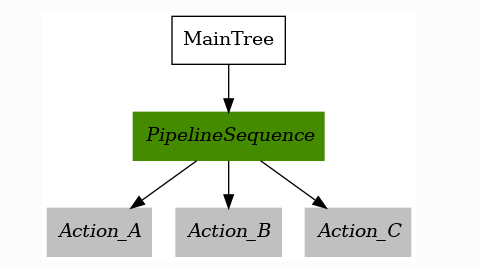
\includegraphics[width=\textwidth]{images/bt_sencillo.png}
    \caption{Estructura de un Árbol de comportamiento básico (Pipeline). Fuente: \cite{nav2}}
    \label{fig:bt_sencillo}
  \end{minipage}
  \hfill
  \begin{minipage}[b]{0.45\textwidth}
    \centering
    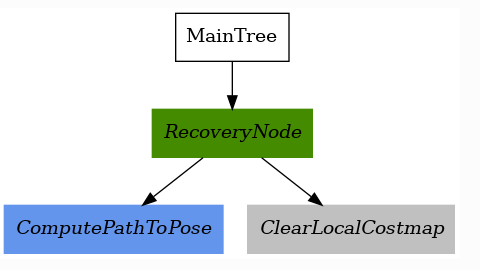
\includegraphics[width=\textwidth]{images/recovery_bt.png}
    \caption{Estructura del nodo de control ''Recovery''. Fuente: \cite{nav2}}
    \label{fig:bt_recovery}
  \end{minipage}
\end{figure}

\subsubsection{Servidores de acción}

Otro concepto clave del stack son los servidores de acción o \textit{action servers} de ROS2, este concepto es fundamental para entender como funciona 
Nav2, estos ''servidores de acción'' cuentan con un \textit{cliente} que hace la petición y con un \textit{servidor} que la realiza y la \textbf{controla}, siendo esto último 
con lo que se diferencian de los servicios de ROS2, en los servidores de acción, el servidor proporciona un flujo constante de mensajes sobre el topic \textit{feedback} 
durante el proceso de ejecución y además tienen la capacidad de ser cancelados en cualquier momento, como se puede ver en la \textbf{figura \ref{fig:servicios_accion}} estos servidores 
generan 3 flujos de datos, el primero un servicio de petición que asegura la llegada de información al servidor, un topic de feedback que devuelve la información durante el proceso y 
un tercero con un servicio de resultado que devuelve el resultado final de ejecución.

\begin{figure}[h]
    \centering
    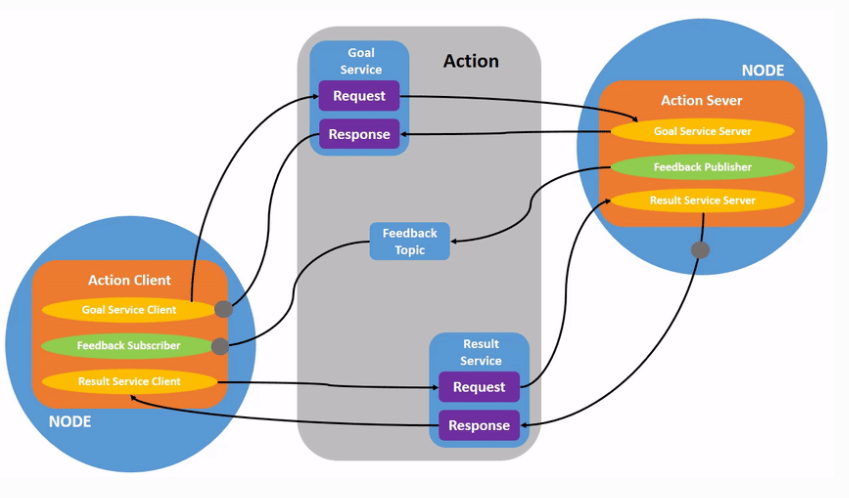
\includegraphics[width=0.5\textwidth]{images/action_server.png}
    \caption{Estructura interna de un servicio de acción o \textit{action server}. Fuente: \cite{ros2}}
    \label{fig:servicios_accion}
\end{figure}

\subsubsection{Estructura para el control de navegación}

En Nav2 todas las funcionalidades están implementadas en forma de servidores de acción y funcionan con una lógica descrita en un árbol de 
comportamiento totalmente modificable.

Estos servidores son 5, \textbf{figura \ref{fig:nav2_arch}}, \textit{Navigator server} que es el encargado de ''leer'' el árbol de comportamiento proporcionado por el usuario y ejecutar las 
diferentes acciones, \textit{Controller server} donde se configura el controlador o ''planificador local'', \textit{Planner server} para configurar 
el planificador o ''planificador global'', \textit{Behavior server} para la selección y configuración de los comportamientos de recuperación 
usados cuando el robot se queda ''atascado'' y por último el \textit{Smoother server} para procesar el camino generado y suavizarlo.

Posteriormente existen 2 mapas de coste, uno local y otro global, el local se encarga de almacenar la información en un entorno reducido y sirve 
para que el controlador haga uso de una buena evitación de obstáculos  y el global para que el planificador genere una trayectoria evitando los obstáculos ya conocidos a más largo alcance.

Finalmente se utilizan 2 plugins externos a la estructura de Nav2, \textit{Velocity smoother} que suaviza los comandos de velocidad para generar movimientos continuos y 
\textit{Waypoint follower} que proporciona la funcionalidad de navegar un array de poses aunque estos estén a mayor distancia del alcance que tiene 
el mapa global, esto lo realian llamando al algoritmo de navegación cada vez que llega a un objetivo, cabe mencionar que las poses deben tener una separación máxima igual o menor al 
alcance del mapa global para que así Nav2 encuentre siempre un camino.


\subsection{Servidores}
\subsubsection{Navigator server}
Para el caso que aquí se expone proporcionaremos un árbol que contiene la lógica para la navegación punto a punto, en la \textbf{figura \ref{fig:bt_ToPose}} observamos un ejemplo proporcionado por 
los creadores del stack para la navegación punto a punto y en la \textbf{figura \ref{fig:bt_ToPose_script}} vemos el mismo ejemplo escrito y modificado en xml para ser usado en 
el proyecto.

\begin{figure}[htbp]
  \centering
  \begin{minipage}[b]{0.7\textwidth}
    \centering
    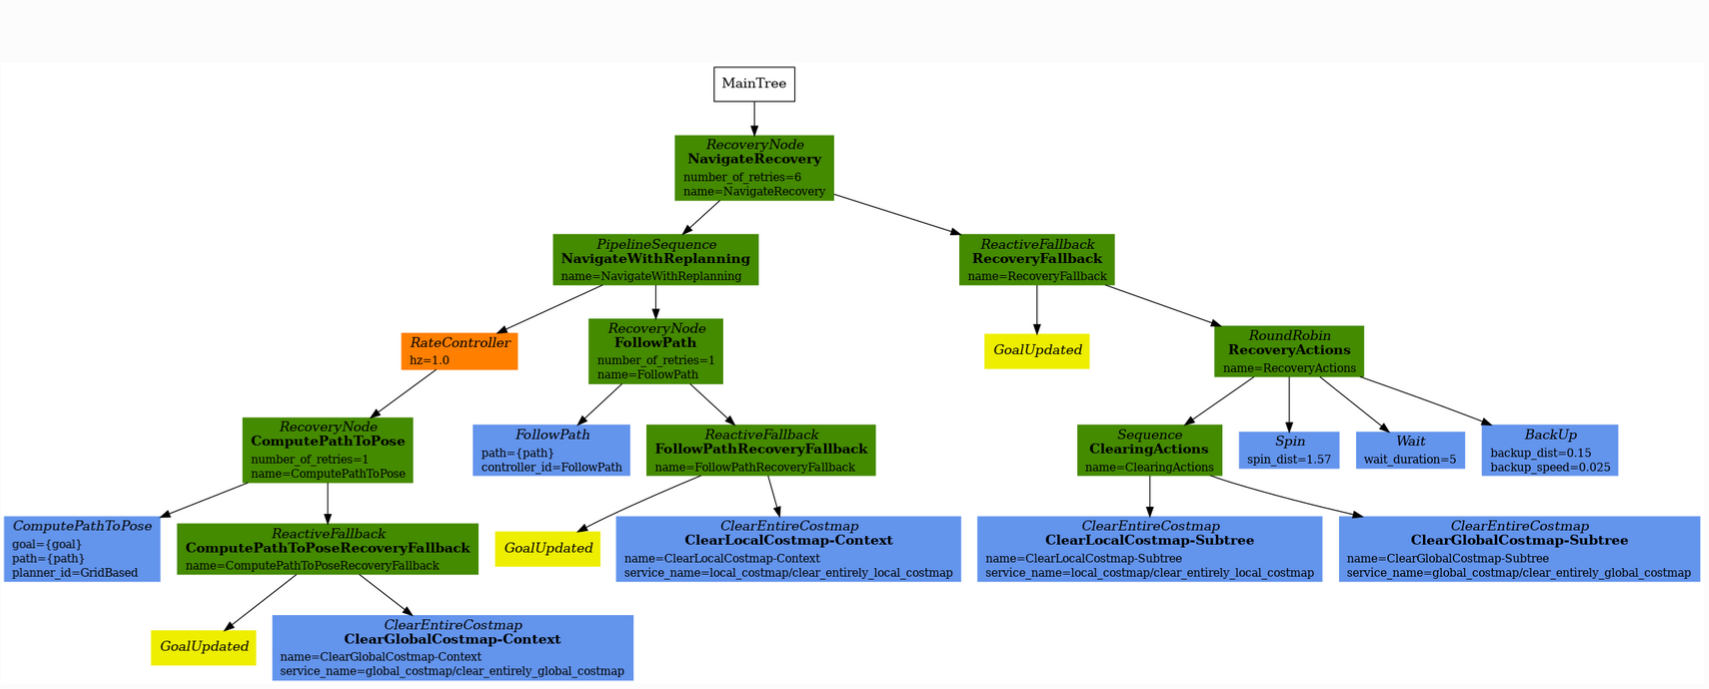
\includegraphics[width=\textwidth]{images/bt_ToPose_wrec_rep.png}
    \caption{Esquema de navegación punto a punto. Fuente: \cite{nav2}}
    \label{fig:bt_ToPose}
  \end{minipage}
  \hfill
  \begin{minipage}[b]{0.7\textwidth}
    \centering
    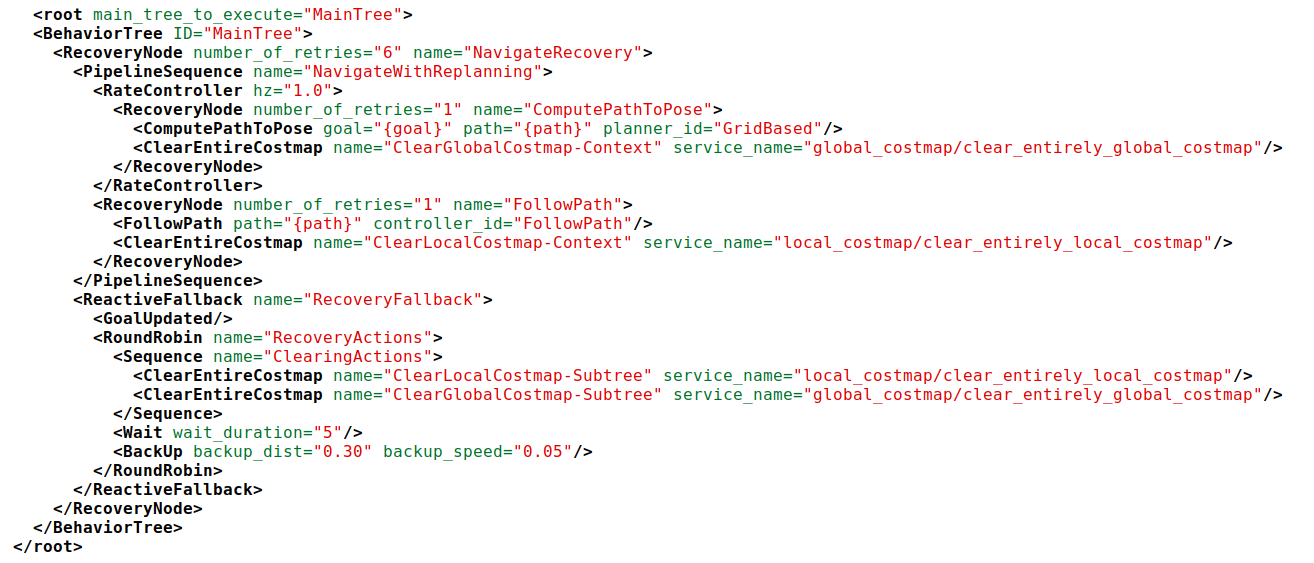
\includegraphics[width=\textwidth]{images/arbol_punto_apunto.png}
    \caption{Código del árbol de comportamiento para la navegación punto a punto. Fuente: propia}
    \label{fig:bt_ToPose_script}
  \end{minipage}
\end{figure}

La funcionalidad básica de esta lógica esta descrita en 2 sub arboles divididos por un nodo de control de tipo ''recovery'', la primera parte intenta navegar 
y la segunda intenta salir de situaciones donde la navegación se imposibilita como esquinas o la aparición de obstáculos dinámicos. En la primera parte 
''computa'' el camino con ayuda de el ''planificador'' y si lo consigue calcular lo sigue con ayuda del controlador, en caso de que no pueda calcularlo o seguirlo 
se procede a borrar el mapa de coste global o local respectivamente.

En el caso de que esto falle se procede al sub árbol de recuperación que incorpora en nuestro caso 2 comportamientos para intentar salir de esa situación de imposibilidad de acción, 
primero borra los 2 mapas de coste y posteriormente con ayuda de un nodo del tipo ''Round Robin'' procede a realizar una parada de 5 segundos (en el caso de que sea una persona andando soluciona el problema de manera rápida) y 
después se mueve hacia atrás 0.15 m, este procedimiento lo intenta 6 veces hasta que se cancela por completo la acción de navegación.

\subsubsection{Behavior server}
Como se ha comentado este servidor cuenta con la posibilidad de configuración de varios comportamientos en caso de que se necesite una recuperación. 
Los que se han usado en el presente proyecto son \textit{clear costmap} que borra el mapa de coste que se seleccione, este comportamiento es 
muy útil cuando aparecen obstáculos dinámicos como podría ser una persona que pasa andando delante del vehículo, ya que borrando el mapa 
de costes forzamos a recalcularlo y evitamos tener que retroceder para encontrar otro camino, el comportamiento de \textit{Wait} hace detenerse al vehículo 
por un determinado tiempo, esto como el anterior proporciona una solución más segura para el caso de obstáculos en movimiento, el último comportamiento 
es \textit{Back up} que simplemente hace al robot dar marcha atrás y así conseguir más espacio para recalcular la trayectoria.

\subsubsection{Controller server}



Como ya se ha comentado en esta memoria, el ''planificador local'' es llamado controlador y es el encargado de hacer que el robot se mueva 
y de que si aparecen obstáculos en el camino, sean dinámicos o no los esquive de manera segura, para la configuración de este servidor se han escogido dos plugins 
que controlan el progreso hacia el objetivo y que detectan la llegada al mismo y también se ha escogido un algoritmo para el propio controlador 
que sea compatible con un robot Ackerman, esto quiere decir que tenga en consideración en radio mínimo de giro. También se ha tenido en cuenta que sea rápido.

Nav2 nos proporciona varias implementaciones para controladores como se puede ver en la \textbf{figura \ref{fig:controllers_tabla}}. 
\begin{figure}[H]
    \centering
    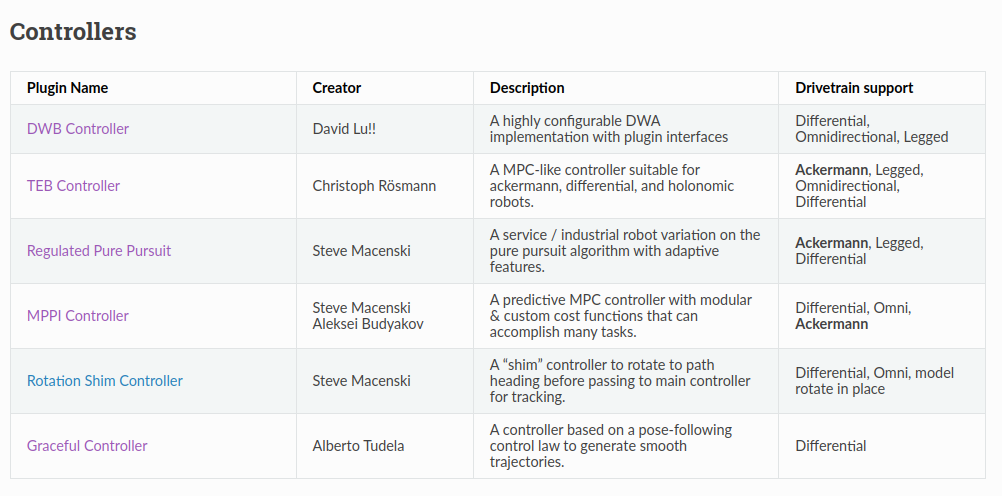
\includegraphics[width=0.5\textwidth]{images/Controllers_tabla.png}
    \caption{Tabla de controladores disponibles para Nav2. Fuente: \cite{nav2}}
    \label{fig:controllers_tabla}
\end{figure}

Lo primero que se hizo fue 
seleccionar los controladores que fuesen compatibles con el robot, estos son \textbf{TEB, Regulated Pure Pursuit y MPPI}, después de una exhaustiva investigación 
se llegó a la decisión de probar el MPPI (Model Predictive Path Integral) por su gran versatilidad en cuanto a configuración, este es un modelo predictivo y una variante del algoritmo \textbf{MPC}, este algoritmo 
es mayoritariamente usado en robots que funcionan a gran velocidad ya que predice la posición del robot en un ''futuro'', al probarlo se descartó por dos 
razones, la primera fue la gran cantidad de parámetros que necesitan ser retocados cuidadosamente para que su configuración lleve a un buen resultado, se llegarón a observar ciertas situaciones en las que no era fiable usarlo, la predicción 
de estados funciona muy bien para casos donde no hay obstáculos o estos se avistan a gran distancia pero en el proyecto resultaba poco fiable, la segunda razón 
es que este algoritmo necesita de una capacidad de cálculo muy grande y se decidió que no compensaba para las muchas funcionalidades que este posee y las pocas 
que se usaban en el proyecto.

Por tanto se probó la segunda opción, el algoritmo \textbf{Regulated Pure Pursuit}, una solución mucho más simple pero 
que daba salida al problema de manera estable, este algoritmo funciona siguiendo unos \textit{objetivos virtuales}, 
\textbf{figura \ref{fig:pure_pursui_teoria}}, pertenecientes a el trayecto a seguir, que se van desplazando conforme el robot se acerca, 
manteniendo una distancia o \textit{look ahead} que puede ser fija o recalculada dinámicamente. En la 
\textbf{figura \ref{fig:rpp_configuracion}} se pueden observar los parámetros escogidos para el algoritmo donde entre ellos se encuentran 
los parámetros típicos de configuración como el \textit{lookahead\_distance} o el radio de giro para las ''incorporaciones'' al trayecto.
\begin{figure}[h]
    \centering
    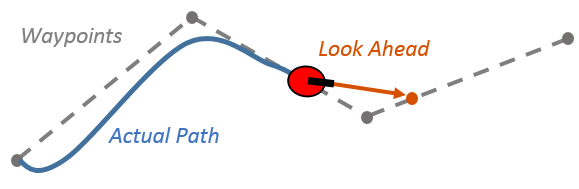
\includegraphics[width=0.5\textwidth]{images/pure_pursuit_teoria.png}
    \caption{Funcionamiento del algoritmo Pure pursuit. Fuente: MathWorks}
    \label{fig:pure_pursui_teoria}
\end{figure}

\begin{figure}[H]
    \centering
    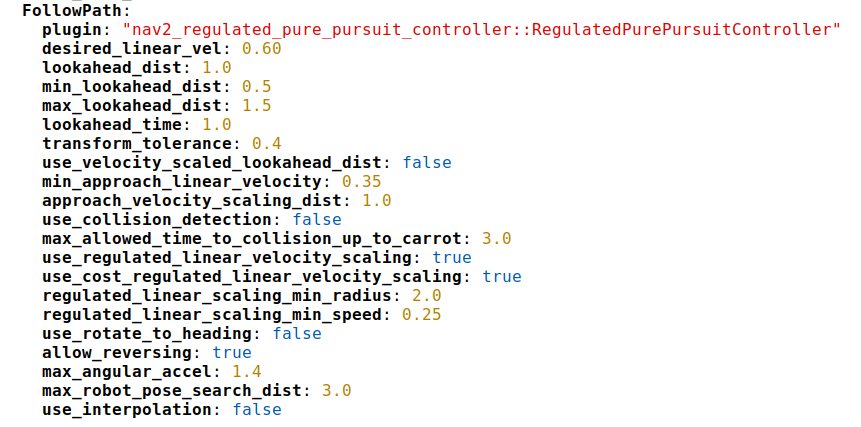
\includegraphics[width=0.5\textwidth]{images/rpp_configuracion.png}
    \caption{Archivo de configuración del algoritmo RPP. Fuente: \cite{nav2}}
    \label{fig:rpp_configuracion}
\end{figure}

\subsubsection{Planner server} 
Para escoger el planificador global se realizo de manera idéntica al controlador, según la \textbf{figura \ref{fig:planificadores_tabla}} podemos ver que las únicas opciones que se tienen son 
\textbf{Smac Planner Hybrid y Smac Planner Lattice}, se procedió a investigar sobre estos algoritmos y la actual implementación de ellos en Nav2, en este caso se escogió 
el \textbf{Smac Planner Hybrid} por la sencilla razón que este algoritmo esta especialmente diseñado para robots de tipo Ackermann y por tanto tiene la opción de habilitar 
la implementación de modelo Reeds-Sheepp, este modelo a diferencia de su opuesto (Dubin) toma en consideración a la hora de generar 
un trayecto la posibilidad de ir marcha atrás, lo que parecía interesante, el Smac Hybrid es una versión modificada 
del conocido \textbf{A*}, un algoritmo de búsqueda recursiva~\cite{dolgov2008practical} que a su vez esta basado en el algoritmo Dijkstra junto con una matriz 
\textit{heurística} para conseguir una solución con mayor rapidez y menor número de búsquedas o iteraciones 
\begin{figure}[H]
    \centering
    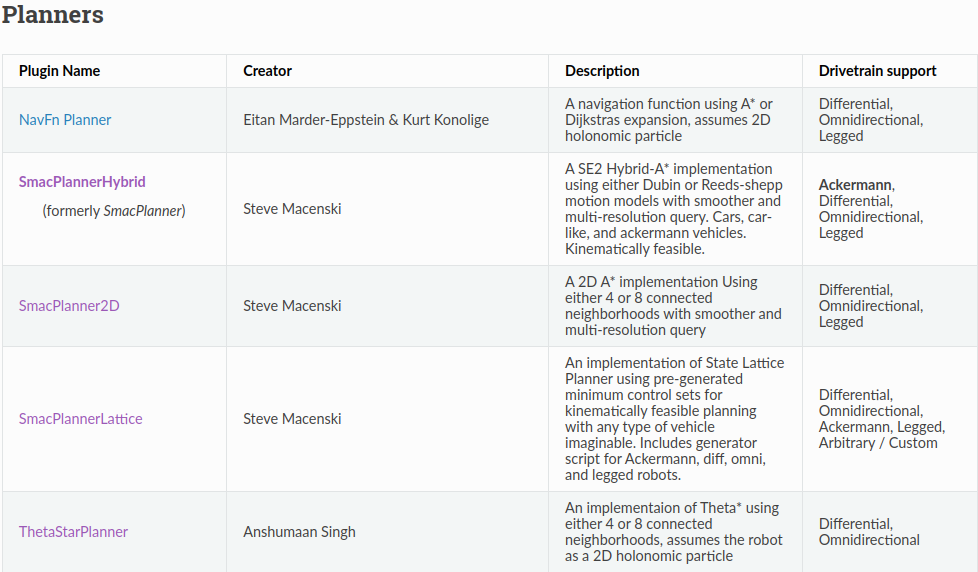
\includegraphics[width=0.5\textwidth]{images/planificadores_table.png}
    \caption{Tabla de planificadores disponibles para Nav2. Fuente: \cite{nav2}}
    \label{fig:planificadores_tabla}
\end{figure}

\newpage
Este algoritmo cuenta con múltiples configuraciones como la ya comentada selección del modelo \textit{Dubin o Reeds-Sheepp}, radio mínimo de giro 
o la selección de las diferentes penalizaciones para los comportamientos del algoritmo como se puede observar en la \textbf{figura \ref{fig:configuracion_planner}}.

\begin{figure}[H]
    \centering
    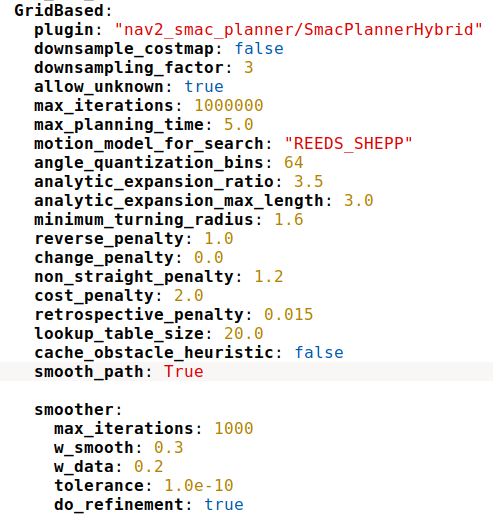
\includegraphics[width=0.3\textwidth]{images/smacplanner_configuracion.png}
    \caption{Archivo de configuración para el planificador Smac Hybrid. Fuente: propia}
    \label{fig:configuracion_planner}
\end{figure}

La selección de estas ''penalizaciones'' ha sido escogida en base a pruebas realizadas con el robot y con la ayuda de las recomendaciones dadas 
por el creador del algoritmo, Steve Macenski~\cite{steve_mc} las cuales se reflejan en \ref{tab:parametros_planificador_steve}

\begin{table}[h!]
    \centering
    \caption{Parámetros de configuración para las penalizaciones del planificador}
    \begin{tabular}{|l|c|}
        \hline
        Penalizaciones     & Rango      \\ \hline
        Penalización de coste          & 1.7 - 6.0  \\ \hline
        Penalización de giro  & 1.0 - 1.3  \\ \hline
        Penalización de cambio de trayectoria        & 0.0 - 0.3  \\ \hline
        Penalización de marcha atrás       & 1.3 - 5.0  \\ \hline
    \end{tabular}
    \label{tab:parametros_planificador_steve}
\end{table}




\subsubsection{Smoother server}
Este servidor es el encargado de suavizar el camino que genera el planificador antes de mandarlo al controlador, así como su implementación es muy necesaria,  
su configuración es muy básica, para sus parámetros se escogió un nodo de suavizado con sus valores por defecto como se ve en la \textbf{figura ~\ref{fig:parametros_smoother_server}}.

\begin{figure}[H]
    \centering
    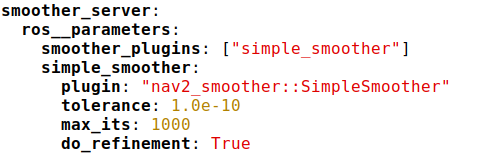
\includegraphics[width=0.5\textwidth]{images/smoother_configuracion.png}
    \caption{Archivo de configuración para el suavizador de trayectorias. Fuente: propia}
    \label{fig:parametros_smoother_server}
\end{figure}

\subsection{Mapas de coste}
Como ya se ha comentado, otra parte importante de la configuración son los mapas de coste donde aquí reside uno de los problemas principales 
a la hora de que Nav2 funcione en exteriores. En una configuración normal uno de los requerimientos básicos para funcionar es proporcionar 
un mapa del entorno estático mapeado \textit{a priori}, tarea imposible para realizar en exteriores. Para solucionar este problema existen múltiples formas 
de proceder, la que se decidió llevar a cabo fue eliminar la capa \textit{estática} en la configuración de los mapas de coste. Estos mapas guardan la 
información sobre los obstáculos actuales y los obstáculos que se han visto a lo largo de la navegación para así poder evitarlos de manera local (evasión de obstáculos) y 
de manera global (generación de una trayectoria que tenga en cuanta esos obstáculos).

El mapa de costes local existe en el sistema de referencia de \textit{odom} y se ejecuta 
a una frecuencia más alta (5 Hz en nuestro caso ), además consta de 2 capas, la primera es una capa ''persistente'' en el tiempo, \textit{voxel}, con la información del Lidar 3D, creando así zonas de obstáculos por 
las que el robot no puede navegar y otra capa no persistente, \textit{inflation}, que infla estos obstáculos de manera exponential creando zonas 
de peligro por donde el robot no debe pasar o al menos pasar a una velocidad reducida para así evitar choques laterales a causa de la forma del robot, \textbf{figura \ref{fig:mapa_local}}, este 
mapa fue creado con un lado igual a 10 m y se añadió un parámetro con las medidas exteriores del robot, esto es un rectángulo, para que de esta manera el controlador tenga en consideración 
la forma del vehículo. En la \textbf{figura \ref{fig:mapa_local}} se distingue en colores vivos el mapa local y por debajo casi transparente el global.

\begin{figure}[H]
    \centering
    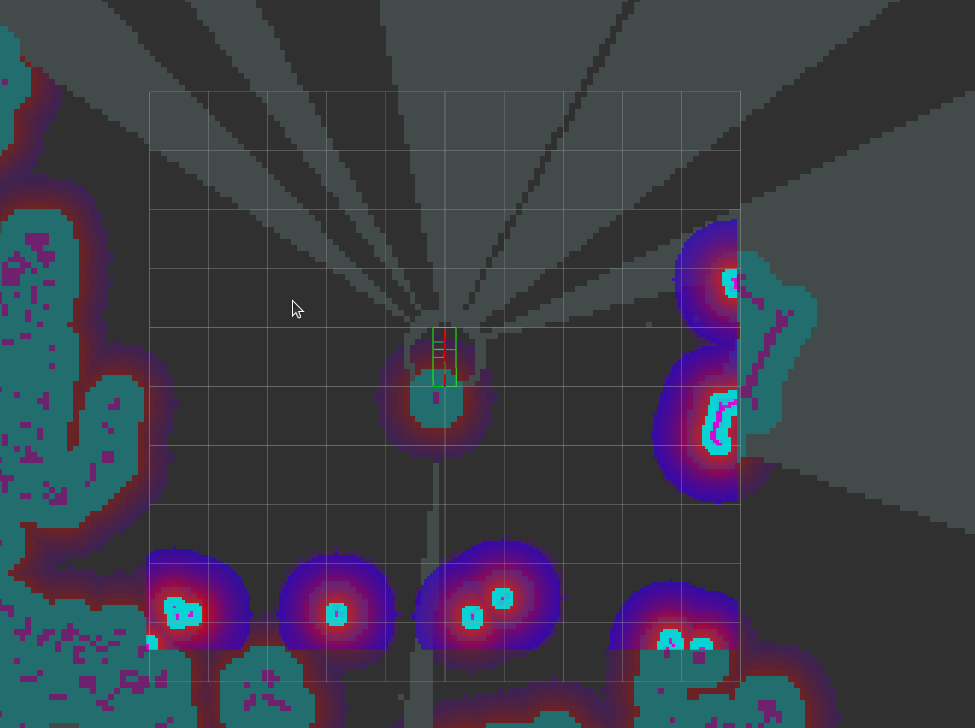
\includegraphics[width=0.5\textwidth]{images/mapa_coste_local.png}
    \caption{Ilustración del mapa de coste local. Fuente: propia}
    \label{fig:mapa_local}
\end{figure}

Para el mapa global se creó otra instancia idéntica pero con un lado igual a 50 m, el sistema de referencia de este mapa sera \textit{/map} y se cambiará 
la capa de \textit{voxel} por la de \textit{Obstacle} que será idéntica a la anterior pero esta será una capa 2D. Además, se 
suscribirá a el topic de \textit{ouster/scan} ya que para el mapa global no necesitamos tanta información del Lidar así como tampoco tanta precisión para el 
cálculo de la trayectoria según las dimensiones del vehículo por lo que se asumirá que el robot es circular para este mapa de costes, \textbf{figura \ref{fig:mapa_global}}.

\begin{figure}[H]
    \centering
    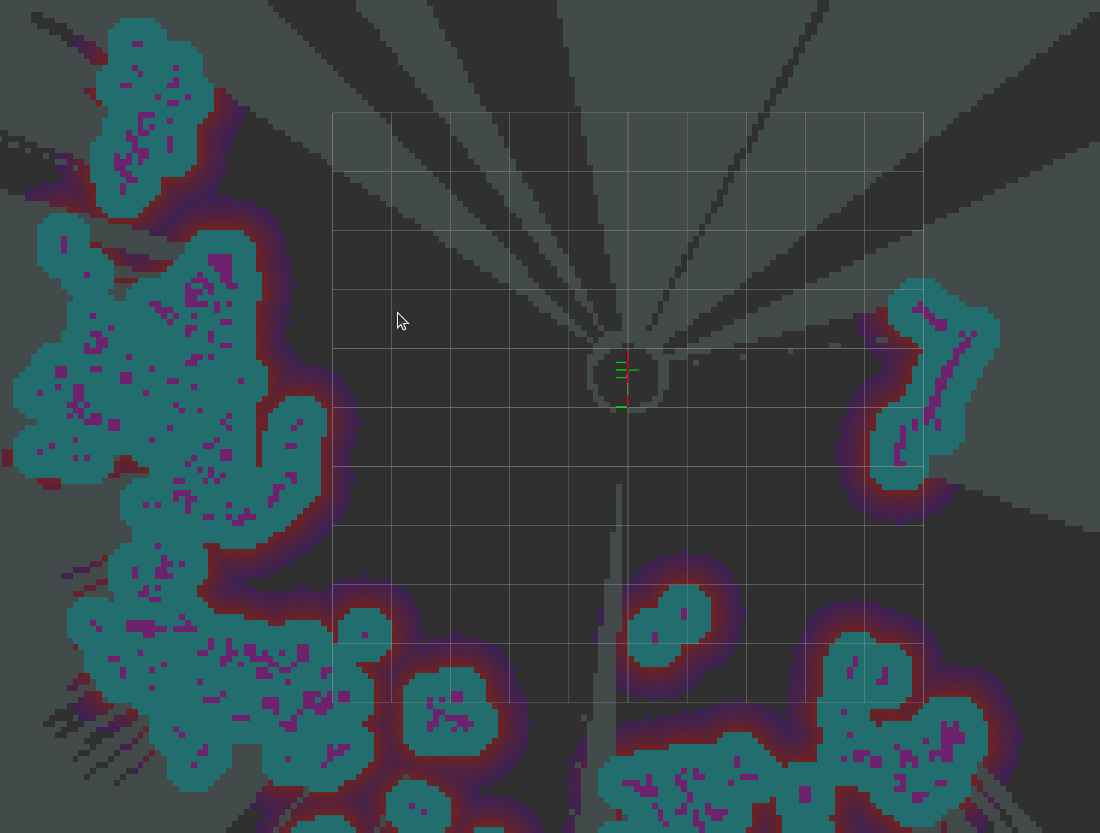
\includegraphics[width=0.5\textwidth]{images/mapa_coste_global.png}
    \caption{Ilustración del mapa de coste global en tonos morados transparentes. Fuente: propia}
    \label{fig:mapa_global}
\end{figure}

\subsection{Plugins}
Los plugins que se han usado son dos, el primero un suavizador final de velocidad donde hemos escogido controlar la velocidad en bucle cerrado y 
hemos seleccionado los rangos de velocidad y aceleración que queremos usar en nuestra aplicación, estos están expresados por 4 vectores como se 
puede apreciar en \textbf{figura \ref{fig:suavizado_vel}} donde los valores se refieren a \begin{math}[\dot{X},\dot{Y},\dot{\theta_{z}}]\end{math} 
 y \begin{math}[\ddot{X}, \ddot{Y}, \ddot{\theta_{z}}] \end{math} respectivamente.

\begin{figure}[H]
    \centering
    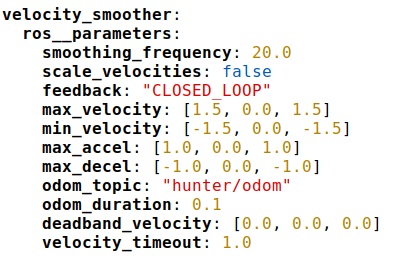
\includegraphics[width=0.5\textwidth]{images/velocity_smoother_configuracion.png}
    \caption{Archivo de configuración para el plugin de suavizado de velocidades. Fuente: propia}
    \label{fig:suavizado_vel}
\end{figure}

En el caso del plugin de \textit{waypoint follower} se tienen solo un par de parámetros, seleccionar que se quiere hacer en cada \textit{waypoint} u 
objetivo (estos pueden esperar a recibir un mensaje por un topic, sacar una foto o pararse durante un tiempo), en el presente proyecto se escogió pararse y se seleccionó 0s de 
duración en la parada para que se cree una trayectoria continua, este plugin ofrece la posibilidad de mandar objetivos que están más lejos que el rango del 
mapa de costes global enviándole un array de poses que estén distanciados cada 2 objetivos una menor disntacia que el rango del mapa de costes global, esto es a razón de 
que este plugin controla el envío del siguiente objetivo del array conforme llega al actual.

\subsection{Nav2 commander}
Como ya se ha comentado en la sección de procesamiento de mensajes, se necesita un procesamiento de las peticiones, estás se podrían clasificar en 3 situaciones, la primera 
donde la distancia al marcador está a menor distancia que el rango del mapa de costes global, en ese caso el procedimiento es sencillo, simplemente se publica la pose por el topic 
\textit{/commander/goal} que es de tipo \textit{/geometry\_msgs/Pose}, si el objetivo esta a más distancia entonces se deberá calcular los puntos intermedios como se puede observar en la 
\textbf{figura \ref{fig:puntos_intermedios}}, en este otro caso publicaremos por el topic \textit{/commander/goal\_array} de tipo \textit{/geometry\_msgs/PoseArray}.


\begin{figure}[H]
    \centering
    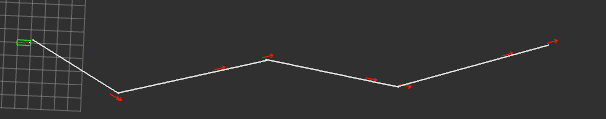
\includegraphics[width=0.5\textwidth]{images/camino_punto_inter.png}
    \caption{Ejemplo de cálculo de puntos intermedios. Fuente: propia}
    \label{fig:puntos_intermedios}
\end{figure}

Nav2 commander es el último nodo realizado para este proyecto y es el encargado de suscribirse a los 2 topics mencionados anteriormente, 
además de otro topic de tipo \textit{/std\_msgs/Bool} llamado \textit{/web/follow} que será \textit{true} cuando el modo ''follow me'' este activo. En 
el caso de recibir un mensaje por el topic \textit{/commander/goal\_array} este se comanda al plugin de \textit{Waypoint follower} por medio de 
una petición de su servidor de acción correspondiente.

En el caso de recibir un mensaje por \textit{/commander/goal} tenemos 2 opciones o el \textit{/web/follow} esta en \textit{false}, donde simplemente 
se hará una petición al servicio propio de Nav2 para navegación punto a punto o que este a \textit{true} donde se deberá hacer uso del mismo servidor pero 
indicando un árbol de comportamiento específico para esta tarea como se observa en la \textbf{figura \ref{fig:follow_me}}.

Este árbol indicará a Nav2 que debe hacer el procedimiento estándar para ir a un punto pero recortando el trayecto 1m para así quedarse siempre a una distancia de la persona, también para hacer más dinámica 
la búsqueda del objetivo las actualizaciones se realizarán por el topic \textit{/goal\_update} del tipo \textit{/geometry\_msgs/PoseStamped}, por tanto 
cuando el ''follow me'' esté activo, los nuevos objetivos enviados por la aplicación web se publicarán por este topic.

\begin{figure}[H]
    \centering
    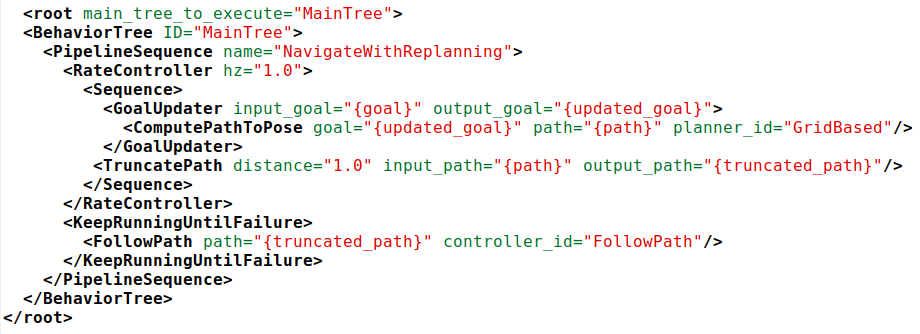
\includegraphics[width=0.5\textwidth]{images/arbol_dynamic.png}
    \caption{Programación en xml del árbol de comportamiento para seguimiento dinámico de una persona (''follow me'')}
    \label{fig:follow_me}
\end{figure}

Hay que resaltar que aunque el algoritmo del ''follow me'' ha sido probado y funciona, este es altamente dependiente de la precisión del GPS 
empleado y ya que los dispositivos móviles tienen una precisión bastante baja, el resultado obtenido no es bueno.
\cleardoublepage
\chapter{Pruebas y resultados}
En el presente capítulo se trata de corroborar que la teoría funciona, poniendo a prueba los algortimo desarrollados. Es decir, que todos los 
sistemas de abordo son efectivos en su trabajo cumpliendo con los requisítos establecidos, para así sacar conclusiones finales sobre las soluciones 
dadas para este proyecto.

\section{Pruebas de precisión para el sistema sensorial}
Para esta prueba se condujeron varios experimentos con la esperanza de encontrar las varianzas de las IMU y así obtener una buena localización.

El primer sensor que se puso a prueba fue la IMU Xsens MTi ya que como se puede ver en la \textbf{figura \ref{fig:xsens_datasheet}}, el fabricante 
proporciona unos valores de ruido que se pueden usar para inducir unos valores en la matriz de covarianza. Por lo que de manera conservadora se tomarán 
estos mismos valores en las diagonales de las matrices.

\begin{minipage}[b]{0.3\textwidth}
    \centering

\begin{itemize}
  \item Orientación
\end{itemize}
$\begin{bmatrix}
  0.475 & 0 & 0\\
  0 & 0.475 & 0\\
  0 & 0 & 0.475
\end{bmatrix}$
\end{minipage}
\hfill
\begin{minipage}[b]{0.3\textwidth}
    \centering

\begin{itemize}
  \item Velocidad Angular
\end{itemize}
$\begin{bmatrix}
  0.005 & 0 & 0\\
  0 & 0.005 & 0\\
  0 & 0 & 0.005
\end{bmatrix}$
\end{minipage}
\hfill
\begin{minipage}[b]{0.3\textwidth}
    \centering


\begin{itemize}
  \item Aceleración Lineal
\end{itemize}

$\begin{bmatrix}
  0.008 & 0 & 0\\
  0 & 0.008 & 0\\
  0 & 0 & 0.008
\end{bmatrix}$

\end{minipage}


Después de varias iteraciones se ajustaron estos valores. Para lo orientación se decidió dejar el valor de 0,475, para velocidad angular se bajó a 0.004 y para la aceleración lineal se subió hasta 
el valor de 0.01. Como se pueden observar en la \textbf{figura \ref{fig:comparacion_covarianza}} la línea azul corresponde a la salida del sensor y 
la roja con menor ruido a la salida del filtro. Concluyendo así, la existencía de una mejora considerable en el error al tener en cuenta estos valores de varianza.



\begin{figure}[H]
    \centering
    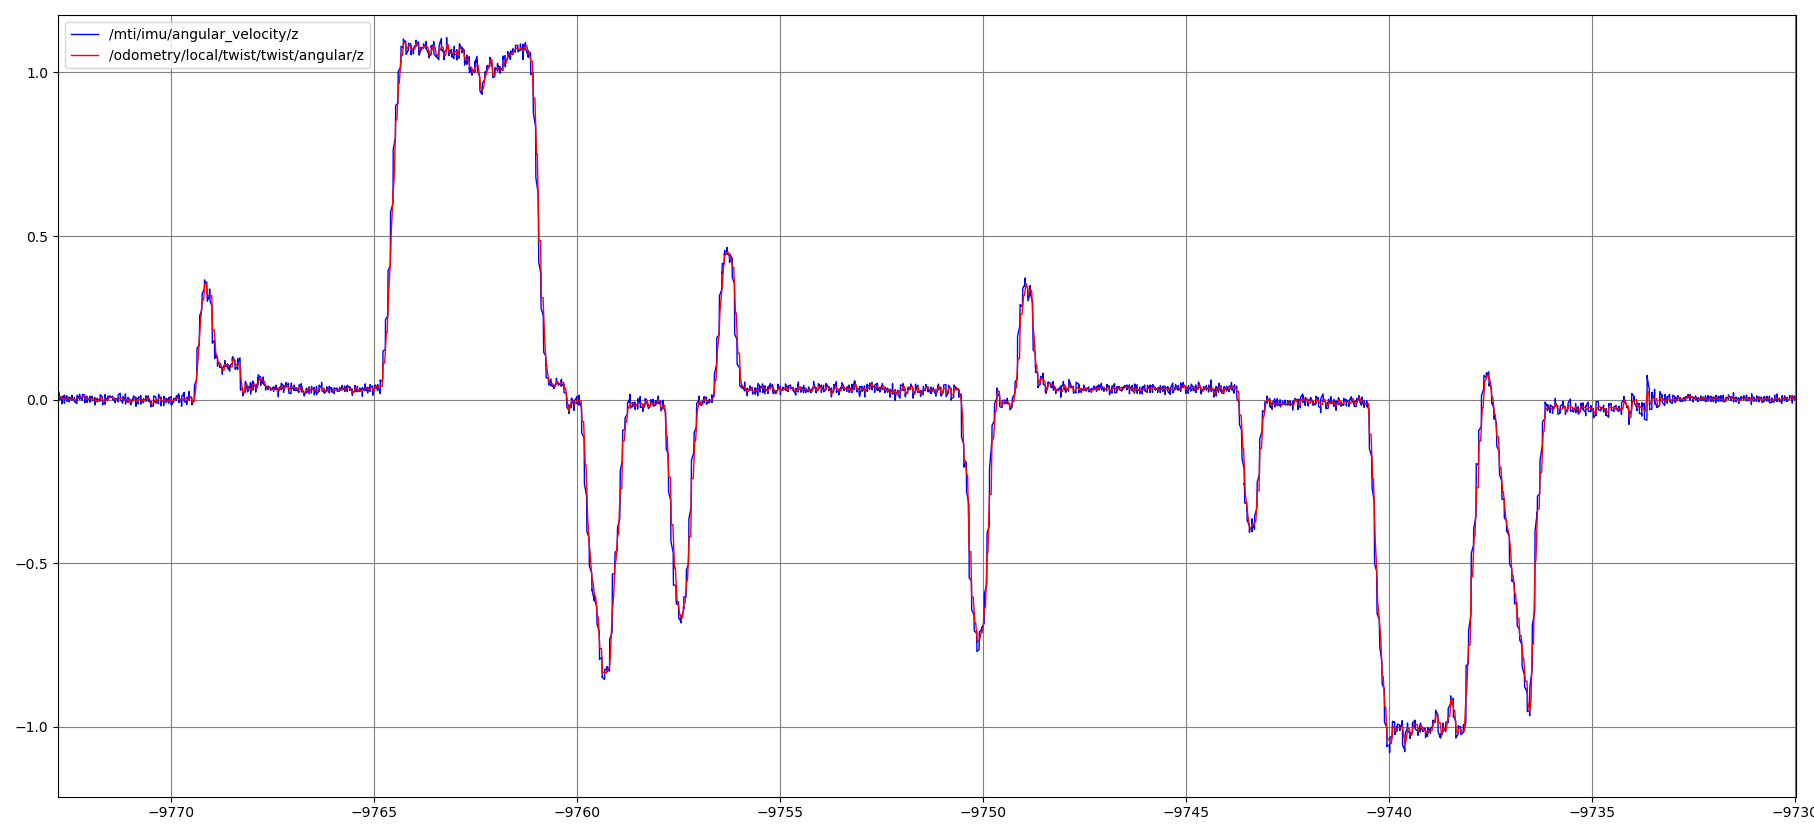
\includegraphics[width=0.8\textwidth]{images/comparacion_mti_covarianza.png}
    \caption{Comparación entre la salida directa del sensor y la salida después de procesarse por el filtro de Kalman con las matrices de covarianza.}
    \label{fig:comparacion_covarianza}
\end{figure}

Para la IMU integrada del Ouster dado los buenos resultados de los valores de la IMU de Xsens se introdujeron los mismos valores de varianza y se implemento el filtro complementario 
para mejorar el error, eliminando el ''bias'' del dispositivo y calculando la orientación en base a su giroscopio y acelerómetro. En la 
\textbf{figura \ref{fig:complementariovsouster}} se puede observar la salida directa del sensor (gris) y la procesada por el filtro complementario (rojo) donde 
se ve claramente un suavizado en la salida junto con la eliminación de gran parte del \textit{offset} o 'bias' que posee la señal sin procesar.

\begin{figure}[H]
    \centering
    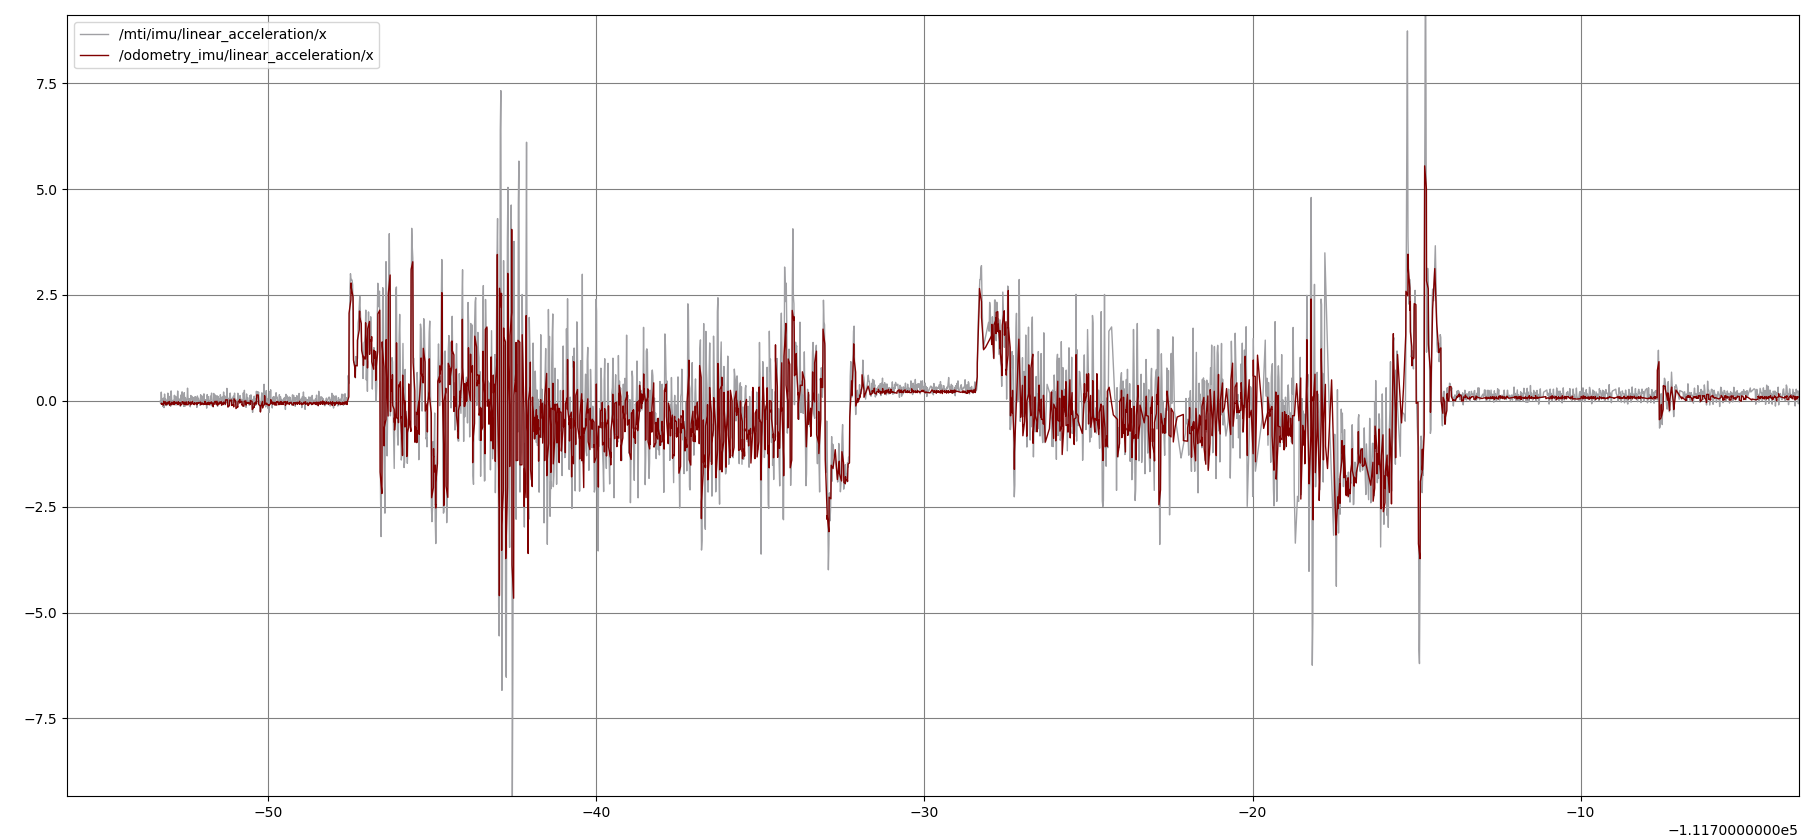
\includegraphics[width=0.8\textwidth]{images/ousterIMu_vscomplementary.png}
    \caption{Comparación entre la salida directa del sensor y la salida del filtro complementario}
    \label{fig:complementariovsouster}
\end{figure}

Para terminar se condujo una prueba de movimiento con el GPS y el RTK conectado para comprobar tanto la configuración del nodo de transformación como 
para corroborar la precisión que puede dar este dispositivo. La información vendrá dada por un mensaje de tipo \textit{NavSatFix}, en concreto el campo  
\textit{Status} de tipo entero, pudiendo ser -1 (cuando no se encuentra solución), 0 (cuando la solución es de tipo ''sencilla'', del orden de 4-5 m 
de error), 1 (cuando la solución es de tipo ''doble'', del orden de 10-50 cm de error) o 2 (cuando la solución es de tipo ''fija'', con el esperado 1 
cm de error), por tanto nos interesa que el GPS se mantenga con un \textit{status} igual a 2.

En las siguientes figuras se puede observar el experimento donde tanto la salida del filtro, \textbf{figura \ref{fig:salida_ekf_rtk}}, como la 
directa del sensor, \textbf{figura \ref{fig:salida_gps_rtk}} permanecen estables, comentar que el offset que existe en la 
\textbf{figura \ref{fig:salida_ekf_rtk}} entre la señal de odometría del robot (rosa) y la salida del filtro de Kalman global(verde) es a causa de 
el procedimiento para el cálculo del datum, donde el robot se mueve una determinada distancia (en este caso se puede apreciar aproximadamente 1m), esto no afecta al filtro ya que esta variable se introduce como relativa (se le resta el valor inicial a todos los posteriores) de manera 
que desde el punto de vista del filtro comienza en 0.

\begin{figure}[htbp]
  \centering
    \captionsetup{skip=0pt}  % Ajusta el espacio entre la figura y la leyenda
  \begin{minipage}[b]{0.45\textwidth}
    \centering

    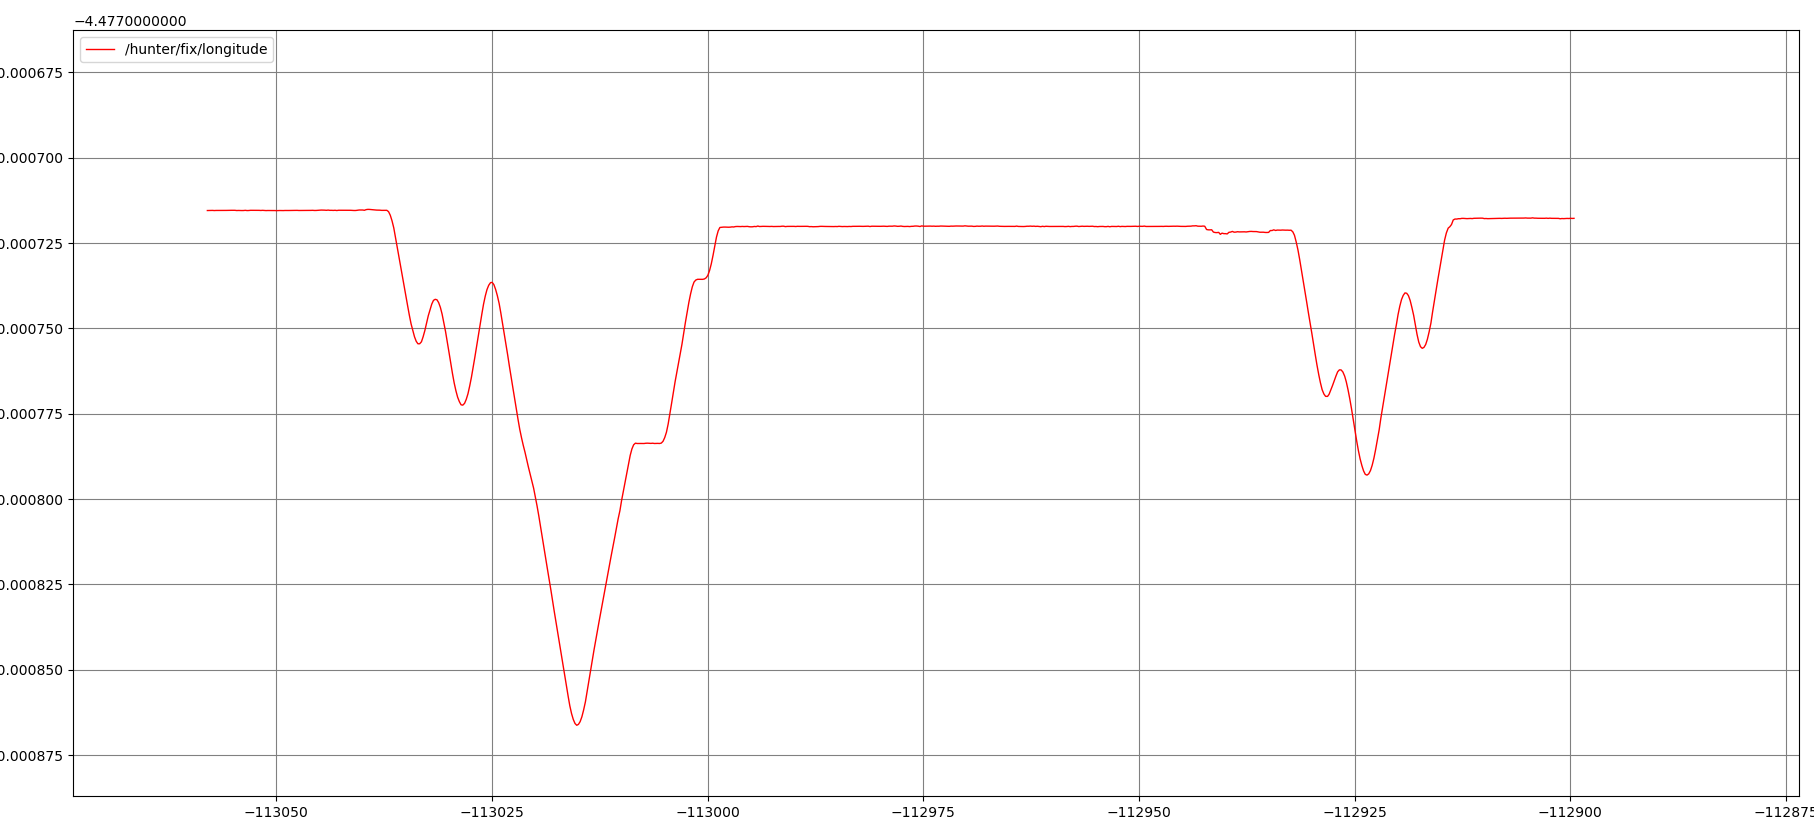
\includegraphics[width=\textwidth]{images/longitude_gps.png}
    \caption{Salida del GPS con RTK.}
    \label{fig:salida_gps_rtk}
  \end{minipage}
  \hfill
  \begin{minipage}[b]{0.45\textwidth} 
    \centering
    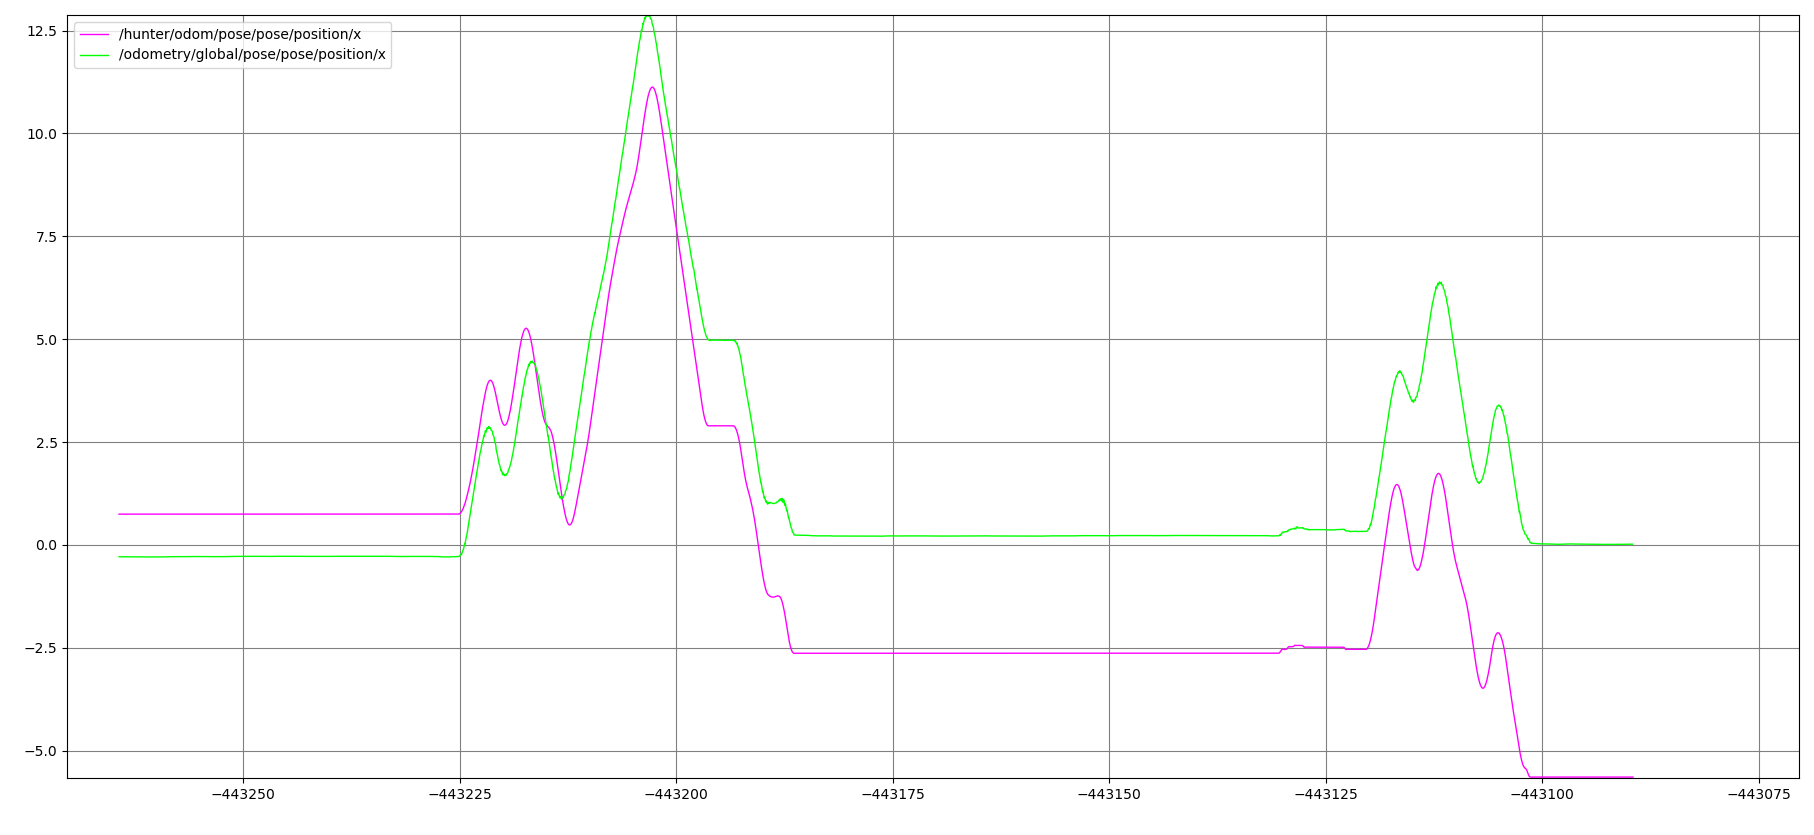
\includegraphics[width=\textwidth]{images/odom_global_rtk.png}
    \caption{Salida del filtro.}
    \label{fig:salida_ekf_rtk}
  \end{minipage}
\end{figure}

\section{Pruebas de funcionamiento de los algoritmos de adaptación}
El primer algoritmo de adaptación es el generador de Datum o \textit{DatumGen}, para esta prueba se quiso comprobar la repetibilidad del algoritmo y 
la precisión a la hora de calcular el ángulo. Para ello se condujeron 2 experimentos, el primero con el robot mirando perfectamente al Oeste donde se probó la 
repetibilidad del sistema y un segundo experimento donde se probó la precisión calculando el ángulo para varios valores de orientación. Para las 2 pruebas 
el robot se moverá a una velocidad constante de 0.8 m/s hacia delante 2 m.

En el primer experimento se realizaron 6 pruebas desde la misma posición inicial.
\begin{table}[H]
    \centering
    \caption{Resultados de repetibilidad del algoritmo}
    \begin{tabular}{|l|c|c|}
        \hline
        Número de prueba     & ángulo de la IMU (rad) & ángulo del algoritmo (rad)     \\ \hline
        1           & 0 & 0 \\ \hline
        2           & 0 & 0  \\ \hline
        3           & 0 & 0  \\ \hline
        4           & 0 & 0  \\ \hline
        5           & 0 & 0  \\ \hline
        6            & 0 & 0  \\ \hline
    \end{tabular}
    \label{tab:repetibilidad_datumgen}
\end{table}

Como se puede ver en la \textbf{tabla \ref{tab:repetibilidad_datumgen}} se consigue una repetibilidad buena con una desviación 
típica de ..............

Para el segundo caso se realizó el experimento para los 360º en intervalos de 90º con los mismos parámetros que en el anterior (0.8 m/s y 2 m de movimiento lineal).

\begin{table}[H]
    \centering
    \caption{Resultados de precisión del algoritmo}
    \begin{tabular}{|l|c|c|}
        \hline
        Dirección     & ángulo de la IMU (rad) & ángulo del algoritmo (rad)     \\ \hline
        Este           & 0 & 0 \\ \hline
        Norte           & 0 & 0  \\ \hline
        Oeste           & 0 & 0  \\ \hline
        Sur           & 0 & 0 \\ \hline
    \end{tabular}
    \label{tab:precisión_datumgen}
\end{table}


Como también se ve en la \textbf{tabla \ref{tab:precisión_datumgen}} se consiguió una precisión de ............ radianes que equivale a ........... grados, siendo estos resultados más que aceptables 
para el proyecto.

El segundo algoritmo a testar será el encargado de generar los arrays de poses en base a las peticiones de objetivos solicitadas por el usuario por medio de 
la web. Para comprobar el correcto funcionamiento sencillamente se harán 2 peticiones, la primera a un punto más alejada que el rango del mapa de coste y la segunda una ruta de una distancia considerable, el algoritmo deberá pintar en Rviz 
todos los objetivos generados con sus orientaciones colocadas correctamente. Como se observa en las 
\textbf{figuras \ref{fig:puntos_intermedios_mas_50m} y \ref{fig:puntos_intermedios_camino}} el resultado es correcto. Además, en el número 1 de la \textbf{figura \ref{fig:puntos_intermedios_mas_50m}} 
observamos el inicio del trayecto y en el 2 el final donde se creo el último objetivo, entremedias se aprecia un marcador adicional corroborando el buen funcionamiento del algoritmo.
\begin{figure}[H]
    \centering
    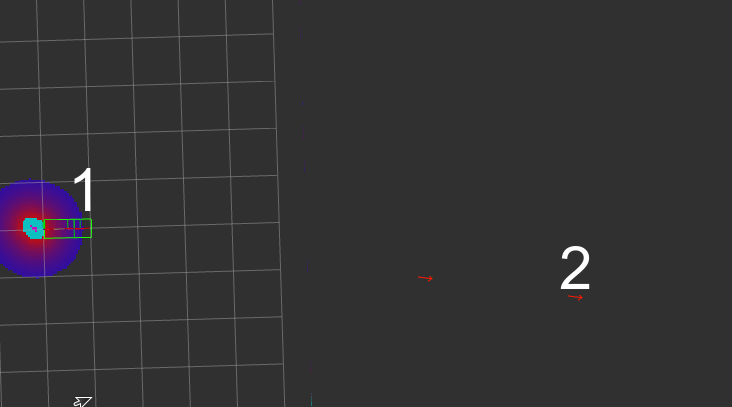
\includegraphics[width=0.6\textwidth]{images/punto_alejado.png}
    \caption{Array de poses objetivos por el algoritmo para una petición de objetivo a más distancia del rango del mapa de coste.}
    \label{fig:puntos_intermedios_mas_50m}
\end{figure}

\begin{figure}[H]
    \centering
    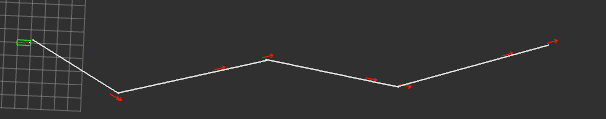
\includegraphics[width=0.8\textwidth]{images/camino_punto_inter.png}
    \caption{Array de poses objetivos generadas por el algoritmo para una petición de camino.}
    \label{fig:puntos_intermedios_camino}
\end{figure}

Como comparación en las siguientes figuras, \textbf{figuras \ref{fig:peticion_punto_alejado} y \ref{fig:peticion_camino}}, se observa la petición enviada por la web donde podemos ver el objetivo único a una distancia considerable y el 
camino creado con la herramienta de linea de la API de google maps ya comentada anteriormente.


\begin{figure}[htbp]
  \centering
  \begin{minipage}[b]{0.45\textwidth}
    \centering
    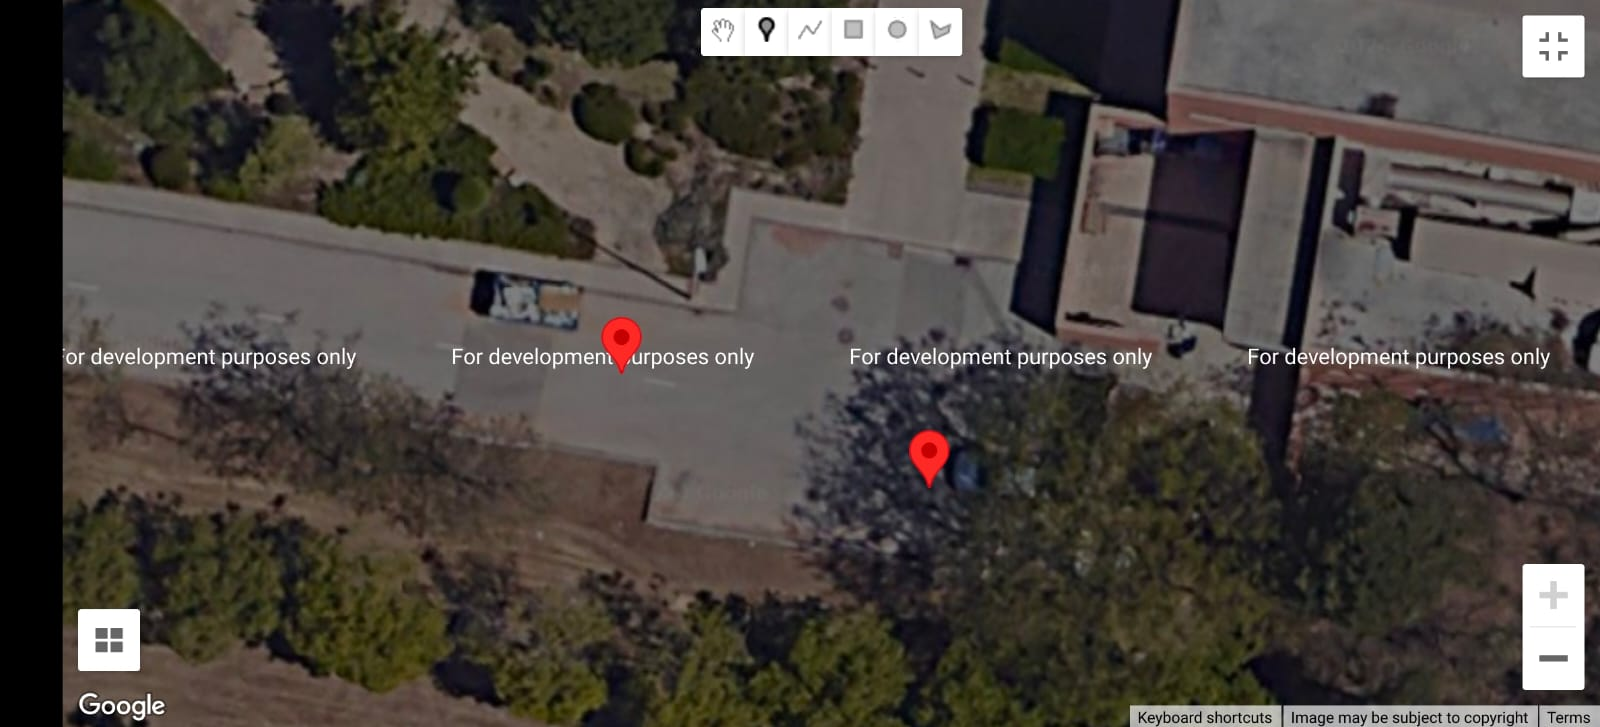
\includegraphics[width=\textwidth]{images/punto_inter_web.jpeg}
    \caption{Petición de navegación a un objetivo más alejado que el rango del mapa de coste.}
    \label{fig:peticion_punto_alejado}
  \end{minipage}
  \hfill
  \begin{minipage}[b]{0.45\textwidth}
    \centering
    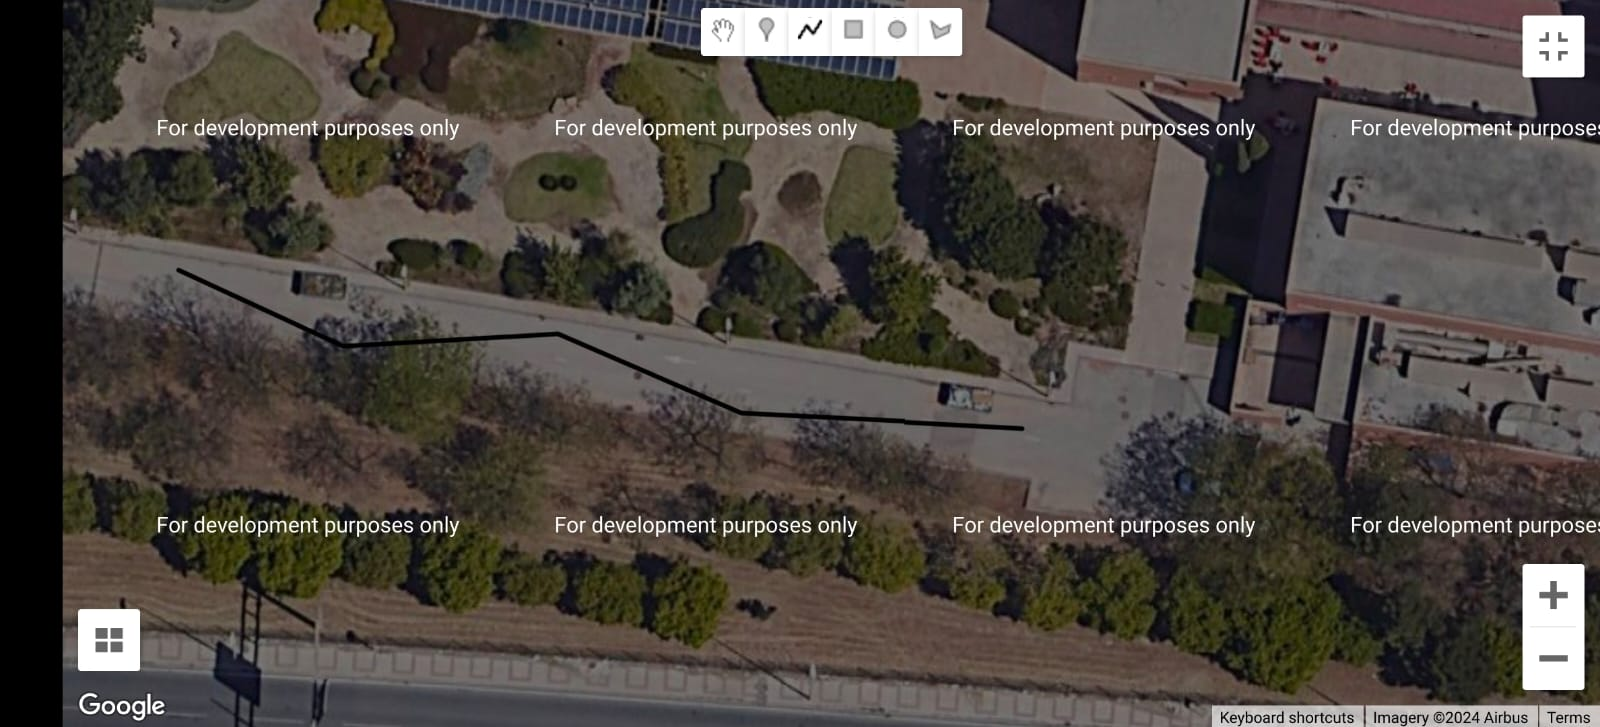
\includegraphics[width=\textwidth]{images/camino_inter_web.jpeg}
    \caption{Petición de navegación para un trayecto establecido.}
    \label{fig:peticion_camino}
  \end{minipage}
\end{figure}


\section{Pruebas de precisión en la localización}

Lo que en este apartado se quiere demostrar es la capacidad que tiene el sistema de localización para mantener una precisión aceptable a lo 
largo del tiempo. Para ello se condujeron 2 experimentos donde para el primero se implemento una localización con 1 sola IMU y se trazó un 
recorrido para comprobar la precisión de estimación, posteriormente se realizó otro experimento donde se introdujeron las 2 IMU en los filtros 
de Kalman, para así comprobar si existe mejora en la orientación. 

Para llegar a una conclusión se utilizó la herramienta de ROS2 \textit{Rviz}, que ayuda a 
ilustrar todo tipo de mensajes de ROS, para esta prueba es necesario centrar la atención en 3 objetos. Como se ve en las 
\textbf{figuras \ref{fig:Localización_1imu} y \ref{fig:localizacion_2imu}} existen 2 flechas, la verde indica la odometría local y la roja la odometría global, estás deben estar siempre 
alineadas, una tendencía a separarse indicaría una diferencia entre el GPS y la odometría, por otro lado también se han 
ilustrado los sistemas de referencia de \textit{odom, map y base\_link}, una buena localización implicará que al final del trayecto la distancia 
entre el sistema de referencia fijo \textit{map} y el sistema \textit{odom} sea pequeña. Por último, se observará la varianza de los filtro de Kalman 
representada por un ''óvalo'' morado alrededor del camino, si crece en tamaño significará que el sistema 
esta perdiendo noción de donde se encuentra. Por lo que el comportamiento ideal que se busca es que el ''óvalo'' permanezca constante en tamaño o al menos que 
crezca de manera paulatina.


\begin{figure}[htbp]
  \centering
  \begin{minipage}[b]{0.45\textwidth}
    \centering
    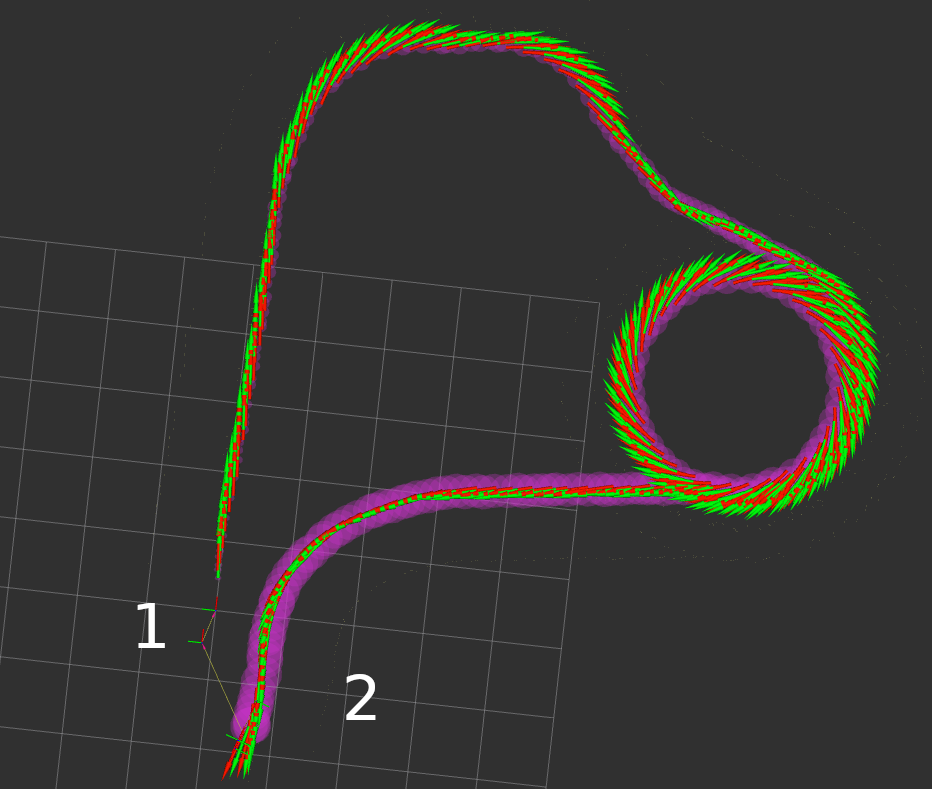
\includegraphics[width=\textwidth]{images/1_imu_final.png}
    \caption{Localización mediante el uso de 1 IMU.}
    \label{fig:Localización_1imu}
  \end{minipage}
  \hfill
  \begin{minipage}[b]{0.4\textwidth}
    \centering
    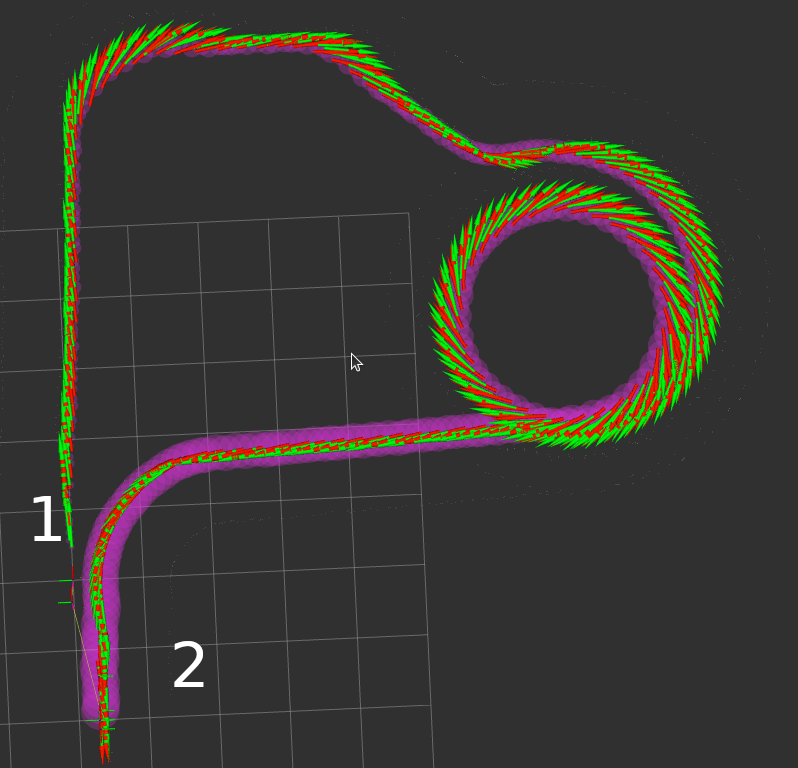
\includegraphics[width=\textwidth]{images/2_imu_final.png}
    \caption{Localización mediante el uso de 2 IMU.}
    \label{fig:localizacion_2imu}
  \end{minipage}
\end{figure}

Como se puede apreciar en las \textbf{figuras \ref{fig:Localización_1imu} y \ref{fig:localizacion_2imu}} tanto el error de estimación como la diferencia entre las 
2 odometrías es práctimante igual para los dos casos. Sin embargo, se puede apreciar una menor deriva en los sistemas de referencia al final del 
trayecto realizado con 2 IMU, esto se observa en el 1 de ambas figuras.
\newpage
\section{Pruebas de navegación autónoma}

Para comprobar finalmente la totalidad del trabajo, en concreto, una navegación cumpliendo con los objetivos propuestos, se desarrollaron 4 escenarios en los que se cubren todas 
las posibilidades de navegación.
\begin{itemize}
  \item Navegación punto a punto.
\end{itemize}
A continuación en las \textbf{figuras \ref{fig:frame1_nav_punto_punto} y \ref{fig:frame2_nav_punto_punto}} se pueden aprecian varios frames del movimiento real del robot para una navegación punto a punto, como referencia este se movió alrededor de 10 metros. En 
las \textbf{figuras \ref{fig:navegacion_punto_punto_web} y \ref{fig:navegacion_punto_punto_rviz}} se comprueba el mismo movimiento ilustrado en Rviz al lado del comando ofrecido por medio de la página web.

\begin{figure}[htbp]
  \centering
  \begin{minipage}[b]{0.5\textwidth}
    \centering
    \includegraphics[width=\textwidth]{images/comando_punto.jpeg}
    \caption{Comando de navegación para un objetivo.}
    \label{fig:navegacion_punto_punto_web}
  \end{minipage}
  \hfill
  \begin{minipage}[b]{0.45\textwidth}
    \centering
    \includegraphics[width=\textwidth]{images/1_punto_naevegacion.png}
    \caption{Representación de navegación punto a punto en Rviz.}
    \label{fig:navegacion_punto_punto_rviz}
  \end{minipage}
\end{figure}

Por tanto se puede comprobar que es capaz de realizar una navegación punto a punto de manera efectiva (el 1 de la \textbf{figura \ref{fig:navegacion_punto_punto_rviz}} es el inicio y el 2 es el final).
\begin{figure}[htbp]
  \centering
  \begin{minipage}[b]{0.45\textwidth}
    \centering
    \includegraphics[width=\textwidth]{images/video_principio_punto_nav.jpeg}
    \caption{frame de video con el robot en la posición de inicio.}
    \label{fig:frame1_nav_punto_punto}
  \end{minipage}
  \hfill
  \begin{minipage}[b]{0.45\textwidth}
    \centering
    \includegraphics[width=\textwidth]{images/video_final_punto_nav.jpeg}
    \caption{frame de video con el robot en la posición final.}
    \label{fig:frame2_nav_punto_punto}
  \end{minipage}
\end{figure}
\newpage
\begin{itemize}
  \item Navegación de trayecto complejo.
\end{itemize}
Para probar una navegación más compleja se comando un trayecto con múltiples objetivos consecutivos, igualmente en las \textbf{figuras \ref{fig:frame1_nav_compleja} y \ref{fig:frame2_nav_compleja}} se observan distintos frames 
del video grabado durante las pruebas realizando este trayecto y en las \textbf{figuras \ref{fig:navegacion_cuadrado_web} y \ref{fig:navegacion_cuadrado_rviz}} se observa de nuevo la odometría en Rviz junto con el comando de navegación enviado por la 
aplicación web.

\begin{figure}[htbp]
  \centering
  \begin{minipage}[b]{0.45\textwidth}
    \centering
    \includegraphics[width=\textwidth]{images/triangulo_navegacion_captura.jpeg}
    \caption{Comando de navegación para un triángulo.}
    \label{fig:navegacion_cuadrado_web}
  \end{minipage}
  \hfill
  \begin{minipage}[b]{0.5\textwidth}
    \centering
    \includegraphics[width=\textwidth]{images/triangulo_nav.png}
    \caption{Representación de navegación compleja en Rviz.}
    \label{fig:navegacion_cuadrado_rviz}
  \end{minipage}
\end{figure}

Como se puede observar en la \textbf{figura \ref{fig:navegacion_cuadrado_rviz}} el 0 corresponde al inicio de movimiento desplazandose hacia cada uno de los objetivos consecutivos. Además, se 
aprecia un desvió entre 2 y 3 de la misma figura, esto es a causa de que el algoritmo de planificación encontró un camino más óptimo a la hora de 
acabar con la orientación deseada en el objetivo, (es decir sin tener que maniobrar como se puede apreciar en 1 o en 2 de la misma figura).

\begin{figure}[htbp]
  \centering
  \begin{minipage}[b]{0.45\textwidth}
    \centering
    \includegraphics[width=\textwidth]{images/triangulo_punto_2_nav_video.png}
    \caption{frame de video con el robot en la posición 2}
    \label{fig:frame1_nav_compleja}
  \end{minipage}
  \hfill
  \begin{minipage}[b]{0.45\textwidth}
    \centering
    \includegraphics[width=\textwidth]{images/triangulo_punto_3_nav.jpeg}
    \caption{frame de video con el robot moviendose de la posición 2 a la 3.}
    \label{fig:frame2_nav_compleja}
  \end{minipage}
\end{figure}

\newpage
\begin{itemize}
  \item Navegación de largo trayecto.
\end{itemize}
En esta prueba el concepto que se quiere demostrar es la capacidad que tiene el sistema de localización en conjunto con el de navegación para mantener un 
buen conocimiento de la posición y orientación del robot. Es decir, que al cabo de un trayecto largo con múltiples objetivos consecutivos la odometría no haya ''derivado'' en 
exceso consiguiendo llegar al objetivo con precisión.
Igualmente que para las otras pruebas observamos en las \textbf{figuras \ref{fig:frame1_nav_largo} y \ref{fig:frame2_nav_largo}} partes del video y en las \textbf{figuras \ref{fig:navegacion_largo_web} y \ref{fig:navegacion_largo_rviz}} se observa 
la representación de la odometría en Rviz junto con el camino propuesto por el usuario mediante la página web.

\begin{figure}[htbp]
  \centering
  \begin{minipage}[b]{0.45\textwidth}
    \centering
    \includegraphics[width=\textwidth]{images/navegacion_largo_trayecto_captura.jpeg}
    \caption{Comando de navegación para un largo trayecto.}
    \label{fig:navegacion_largo_web}
  \end{minipage}
  \hfill
  \begin{minipage}[b]{0.45\textwidth}
    \centering
    \includegraphics[width=\textwidth]{images/nav_larga_2.png}
    \caption{Representación de navegación de largo trayecto en Rviz.}
    \label{fig:navegacion_largo_rviz}
  \end{minipage}
\end{figure}

Al igual que el resto de pruebas, esta también demostró unos buenos resultados a la hora de maniobrar largas distancias. En 3 de la \textbf{figura \ref{fig:navegacion_largo_rviz}} 
se aprecia un pequeño desvio del trayecto al igual que en otras partes del recorrido, esto es debido a que el robot en estos casos debe maniobrar para llegar a los objetivos intermedios con la orientación correcta.
\begin{figure}[htbp]
  \centering
  \begin{minipage}[b]{0.45\textwidth}
    \centering
    \includegraphics[width=\textwidth]{images/inicio_nav_larga.png}
    \caption{frame de video con el robot en la posición de inicio.}
    \label{fig:frame1_nav_largo}
  \end{minipage}
  \hfill
  \begin{minipage}[b]{0.45\textwidth}
    \centering
    \includegraphics[width=\textwidth]{images/final_nav_larga.png}
    \caption{frame de video con el robot en la posición final.}
    \label{fig:frame2_nav_largo}
  \end{minipage}
\end{figure}

\newpage
\begin{itemize}
  \item Navegación con evitación dinámica de obstáculos.
\end{itemize}
Por último se quiere demostrar que el robot es capaz de navegar de manera autónoma evitando obstáculos dinámicos en su camino. Para ello se procedió a comandar al robot moverse 
a un objetivo arbitrario y para simular un obstáculo se paso por delante del robot primero andando sin detenerse muy lentamente y después parándose en su camino.
Este comportamiento se puede observar en los frames del video (\textbf{figuras \ref{fig:frame1_dinamica} y \ref{fig:frame2_dinamica}}) y también 
en la representación de Rviz en la \textbf{figura \ref{fig:navegacion_dinamica_rviz}}. Aclarar que los puntos rojos en esta misma figura muestran donde se paso por delante del robot, siendo en 1 donde se interrumpio su camino de manera rápida (andando sin detenerse), 
esperando ver como el robot simplemente espera 5 segundos para después seguir su camino y en 2 y 3 donde se pasó delante del robot simulando un obstáculo fijo para así comprobar como este después de esperar y dar marcha atrás, recalcula su 
trayecto esquivándolo de manera efectiva.


\begin{figure}[H]
    \centering
    \includegraphics[width=0.6\textwidth]{images/esquivando_nav.png}
    \caption{Representación de navegación con evitación dinámica de obstáculos en Rviz.}
    \label{fig:navegacion_dinamica_rviz}
\end{figure}

En la \textbf{figura \ref{fig:navegacion_dinamica_rviz}} se puede apreciar muy claramente el funcionamiento de los comportamientos comentados 
en el capítulo anterior (wait, Back up) donde en 1 no se aprecia casí movimiento ante el obstaculo, simplemente se espero y desvió un poco su trayectoria. Por otro lado, 
el 2 y en 3 a causa de la persistencia del obstáculo decició maniobrar hacia atrás para posteriormente evitarlo.

\begin{figure}[htbp]
  \centering
  \begin{minipage}[b]{0.45\textwidth}
    \centering
    \includegraphics[width=\textwidth]{images/evitacion_video_inicio.jpeg}
    \caption{frame de video con el robot parado a causa de un nuevo obstáculo.}
    \label{fig:frame1_dinamica}
  \end{minipage}
  \hfill
  \begin{minipage}[b]{0.45\textwidth}
    \centering
    \includegraphics[width=\textwidth]{images/evitacion_video_final.jpeg}
    \caption{frame de video con el robot esquivando el obstáculo.}
    \label{fig:frame2_dinamica}
  \end{minipage}
\end{figure}

Como se ha podido comprobar el vehículo autónomo consigue llegar a todos los objetivos de manera precisa y segura completando así todas las pruebas con éxito y por tanto 
cumpliendo todos los objetivos propuestos en este trabajo.

\chapter{Conclusiones}
Durante el presente proyecto se ha desarrollado una interfaz de control que cumple con los objetivos propuestos; es funcional y fácil de usar, 
se ha implementado el envió y procesamiento de todas las posibles funcionalidades propuestas.

Se han desarrollado algoritmos de adaptación tanto de sensores como para la mejora de la localización con buenos resultados en la fiabilidad del sistema, donde el cálculo 
de la orientación por medio del movimiento del robot a resultado de tener una precisión más que aceptable.

En cuento a la localización se ha conseguido mantener una buena precisión a lo largo de un tiempo y una distancia considerable, habiéndola probado durante más de 1 hora 
y recorriendo algo más de 1 km continuado, habiendo comprobado también
que es fiable incluso bajo pérdidas momentáneas de la señal RTK del GPS o incluso de la propia señal GPS durante varios segundos.

La navegación ha resultado también bastante fiable consiguiendo que realize cambios de dirección con la aparición de obstáculos dinámicos y sea capaz de 
llegar a su objetivo con un error menor a unas decenas de centímetros.

Este sistema ha sido desarrollado de manera ampliable y sobre todo para que sea utilizado en los futuros proyectos del departamento, 
siendo este proyecto una solución completa y robusta para ello.

\chapter{Futuras líneas de trabajo}

Este proyecto presenta aunque aceptable para el alcance de el trabajo, una carencia en localización para ser un vehículo de exteriores, 
una vía de trabajo que considero mejoraría enormemente este tema sería la caracterización de los sensores IMU, consiguiendo así unos 
valores precisos de varianza para cada estado del sistema, dado que estas han sido impuestas de manera fija y escogidas con poco 
razonamiento teórico.

Otro campo que consideró mejoraría este proyecto sería el desarrollo de los comentados \textit{behavior} o comportamientos específicos para 
el modelo Ackermann ya que actualmente los únicos que existen son \textit{Wait} y \textit{Back up} y aunque suficientes para conseguir una navegación buena,
la creación de un comportamiento que retroceda de manera más ''inteligente'' ayudaría en gran medida a la fluidez del sistema.

Para el caso del ''follow me'' definitivamente se debería buscar otra manera de realizarlo sea con un gps externo o con ayuda de algún tipo de 
detección de personas por medio de cámaras o por medio de la reflectancia de el Lidar.

Por último, sería interesante ampliar las funcionalidades de navegación, como podría ser un barrido de areas, para ello sería necesario 
la creación de algoritmos para la generación de trayectorias dadas las areas.